\documentclass[xcolor={rgb,x11names,svgnames},rgb,x11names,svgnames]{beamer}

%\includeonlyframes{lu,sca-lu}

\usepackage[T1]{fontenc}
\usepackage{cellspace}

\usepackage{amsmath}
\DeclareMathOperator*{\argmax}{arg\,max}

\usepackage{amsfonts}
\usepackage{tikz}
\usepackage{xspace}
\usepackage[normalem]{ulem}
\usepackage{minted}
\definecolor{codebg}{rgb}{0.95,0.95,0.95}
\setminted{bgcolor=codebg}
\usepackage{changepage}
\usepackage[absolute,overlay]{textpos}


\newenvironment{wider}{%
\begin{adjustwidth}{-0.6cm}{}%
  \begin{minipage}{12cm}%
}{%
\end{minipage}%
\end{adjustwidth}%
}

\usepackage{ifthen}


\usepackage{marvosym}
\usepackage{pifont}
%\usepackage[rgb]{xcolor}

\newcommand{\bigO}[1]{\ensuremath{\mathcal{O}\left( #1 \right)} }
\newcommand{\bigOmega}[1]{\ensuremath{\Omega\left( #1 \right)} }
\newcommand{\triste}{\includegraphics[width=0.5cm,trim=0 17mm 0 0]{triste}}
\newcommand{\smiley}{\includegraphics[width=0.5cm,trim=0 17mm 0 0]{content}}

\newcommand{\red}{\alert}
\newcommand{\green}{\color{LimeGreen}}
\newcommand{\blue}{\color{cyan}}

% FORTIN
\newcommand{\mynote}[1]{\note<1>[item]{#1}}
\newcommand{\euro}{\EUR\xspace}

\usetikzlibrary{patterns}
\usetikzlibrary{snakes}
 \usetikzlibrary{arrows}
\usetikzlibrary{backgrounds}
\usetikzlibrary{shapes}
\usetikzlibrary{shadows}
\usetikzlibrary{shadings}
\usetikzlibrary{calc}
\usetikzlibrary{decorations}
\usetikzlibrary{decorations.pathmorphing}
\usetikzlibrary{decorations.shapes}
\usetikzlibrary{decorations.markings}
\usetikzlibrary{positioning}
\usetikzlibrary{math}

\definecolor{amethyst}{rgb}{0.6, 0.4, 0.8}
\definecolor{cyan}{rgb}{0,0.6796875,1}

\usecolortheme{rose}
\setbeamertemplate{footline}{}
\setbeamertemplate{navigation symbols}{}

  \newcommand{\tikzmat}[2] {
\draw[thick] let \p1 = (#1 |- #2),
                 \p2 = (#2 |- #1) in
   ($ (#1) + (0.05,-0.1) $) -- ++(-0.15, 0)  -- ($ (\p1) + (-0.1,0.1) $) -- ++(0.15,0)
   ($ (\p2) + (-0.05,-0.1) $) -- ++(0.15, 0) -- ($ (#2) + (0.1,0.1) $) -- ++(-0.15,0);
}
  


\usepackage{fontspec}

\setsansfont{PalatinoSansLTPro}[
   Path = /home/charles/charles_work/fonts/PalatinoSans/, 
   %Path = ../PalatinoSans/, 
   Extension      = .otf,
   UprightFont    = *-Regular,
   BoldFont= *-Bold ,
   ItalicFont = *-Italic,
   BoldItalicFont = *-BoldIta
]

\title{Lecture 4: Common Algorithmic Themes}

\begin{document}

\begin{frame}[label=title]
  \titlepage
\end{frame}

\section{Généralités}

%%%%%%%%%%%%%%%%%%%%%%%%%%%%%%%%%%%%%%%%%%%%%%%%%%%%%%%%%%%%%%%%%%%%%%
\begin{frame}
\frametitle{How to Write Efficient Parallel Programs?}

\begin{block}{General principles}

\begin{itemize}
\item \textbf{Data locality}: minimize communications by placing data near the CPUs that need them

\medskip

\item \textbf{load balancing}: minimize periods of inactivity

\medskip

\item \textbf{Overlap communication with computation}: avoid processors sitting
  idle while transferring data
\end{itemize}
\end{block}

\end{frame}


%%%%%%%%%%%%%%%%%%%%%%%%%%%%%%%%%%%%%%%%%%%%%%%%%%%%%%%%%%%%%%%%%%%%%%
\begin{frame}
  \frametitle{Load balancing}

  ``Load balancing'' = who does what? = affecting tasks to CPU
  
  \begin{exampleblock}{Predictable workload}
    \begin{itemize}
    \item[$\Rightarrow$] \textbf{Static} job affectation
      \begin{itemize}
      \item[$=$] Can be determined in advance, fixed over time
      \end{itemize}
      
    \item Typical scenario: 
      \begin{itemize}
      \item All data requiring the same amount of computation time
      \item[$\rightarrow$] Distributed by block, cyclic, \dots
      \end{itemize}
    \end{itemize}
  \end{exampleblock}
  
  \medskip
  
  \begin{alertblock}{Unpredictable workload}
    \begin{itemize}
    \item[$\Rightarrow$] \textbf{Dynamic} load balancing
      \begin{itemize}
      \item Affectation of tasks to processes \emph{during} the computation
      \end{itemize}
    \item \sout{Master-slave} Boss-worker paradigm
    \item ``Work stealing'' paradigm
    \end{itemize}
  \end{alertblock}
\end{frame}


%%%%%%%%%%%%%%%%%%%%%%%%%%%%%%%%%%%%%%%%%%%%%%%%%%%%%%%%%%%%%%%%%%%%%%
\begin{frame}
  \frametitle{\sout{Master-Slave} Boss-Worker  Model}

  \begin{itemize}
  \item The boss knows the data and the work to be done
  \item Available workers ask for work
  \item The boss sends tasks (or orders the workers to stop)
    \begin{alertblock}{Limitations}
      \begin{itemize}
      \item The boss needs a lot of RAM if they have to load all the data
      \item 2 message exchanges per task (A/R) $\longrightarrow$ high granularity
      \item Too many workers $\rightarrow$ the boss becomes a bottleneck
      \end{itemize}
    \end{alertblock}
    
    \begin{exampleblock}{Advantages~:}
      \begin{itemize}
      \item Good load balancing, even with heterogeneous resources (or availability/speed that varies with time)
      \item \emph{Checkpointing} is very easy (checkpoint the boss)
      \end{itemize}
    \end{exampleblock}
  \end{itemize}
\end{frame}


%%%%%%%%%%%%%%%%%%%%%%%%%%%%%%%%%%%%%%%%%%%%%%%%%%%%%%%%%%%%%%%%%%%%%%
\begin{frame}
  \frametitle{Work-Stealing Model}

  \begin{exampleblock}{Principle}
    
    \begin{itemize}
    \item Each processor manages their own work list
      
      \begin{itemize}
      \item \textit{A priori} fair initial distribution
      \end{itemize}
      
    \item If task list is empty :
      \begin{itemize}
      \item Choose a \emph{victim} (randomly?)
      \item ``Steal'' a fraction (50\% ?) of the victim's remaining work
      \end{itemize}
    \end{itemize}
  \end{exampleblock}
  
  \bigskip
  
  \begin{itemize}
  \item [+] Completely symmetrical
    \begin{itemize}
    \item ``\textit{No gods, no masters}'' \CircledA
    \end{itemize}
    
  \item [+] Every process participates in the calculation
    \begin{itemize}
    \item No \sout{parasite} bosses twiddling their thumbs
      
    \end{itemize}
  \item [--] not easy to detect when the computation is terminated
  \item [--] difficult to program
  \item [--] difficult to \emph{checkpoint}
  \end{itemize}
\end{frame}

%%%%%%%%%%%%%%%%%%%%%%%%%%%%%%%%%%%%%%%%%%%%%%%%%%%%%%%%%%%%%%%%%%%%%

%%%%%%%%%%%%%%%%%%%%%%%

\begin{frame}
  \frametitle{Overlapping Communication and Computation}

  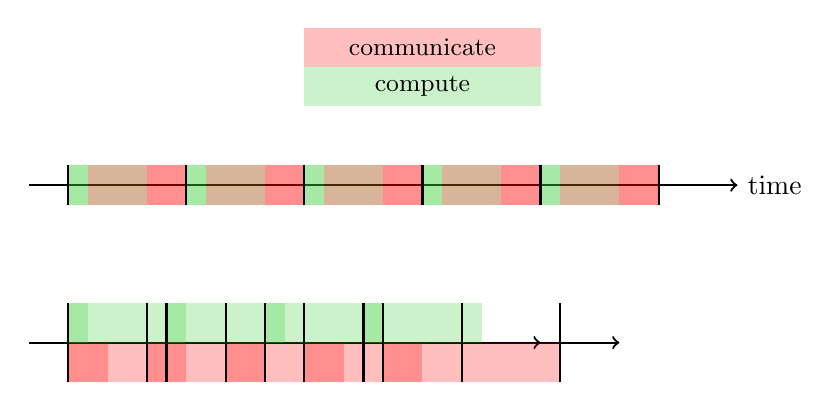
\begin{tikzpicture}
    % initial 
    \draw[thick, ->] (-0.5, 0) -- (8.5, 0) node[right] {time};
    \foreach \i in {0, 1, 2, 3, 4}  {
      % longer comms
      \fill<1>[fill=LimeGreen, nearly transparent] (\i*1.5cm, -0.25) rectangle +(1, 0.5);
      \fill<1>[fill=red, nearly transparent] (\i*1.5cm + 1cm, -0.25) rectangle +(0.5, 0.5);
      % longer comms
      \fill<2>[fill=LimeGreen, nearly transparent] (\i*1.5cm, -0.25) rectangle +(0.25, 0.5);
      \fill<2>[fill=red, nearly transparent] (\i*1.5cm + 0.25cm, -0.25) rectangle +(1.25, 0.5);
    }
    \foreach \i in {0, 1, 2, 3, 4, 5} {
      \draw[thick] (\i*1.5cm, -0.25) -- +(0, 0.5);
    }

    \begin{scope}[yshift=-2cm]
      % overlap, longer compute
      \draw<1>[thick, ->] (-0.5, 0) -- (6, 0);
      \draw<2>[thick, ->] (-0.5, 0) -- (7, 0);
      \foreach \i in {0, 1, 2, 3, 4}  {
        \fill<1>[fill=LimeGreen, nearly transparent] (\i*1cm, 0) rectangle +(1, 0.5);
        \fill<1>[fill=red, nearly transparent] (\i*1cm, -0.5) rectangle +(0.5, 0.5);

        \fill<2>[fill=LimeGreen, nearly transparent] (\i*1.25cm, 0) rectangle +(0.25, 0.5);
        \fill<2>[fill=red, nearly transparent] (\i*1.25cm, -0.5) rectangle +(1.25, 0.5);

      }
      \foreach \i in {0, 1, 2, 3, 4, 5} {
        \draw<1>[thick] (\i*1cm, -0.5) -- +(0, 1);
        \draw<2>[thick] (\i*1.25cm, -0.5) -- +(0, 1);
      }
    \end{scope}
  
    \begin{scope}[xshift=2cm]   % legend
      \fill[fill=LimeGreen, nearly transparent] (1, 1) rectangle +(3, 0.5);
      \path (1, 1) rectangle node[font=\small] {compute} +(3, 0.5);

      \fill[fill=red, nearly transparent] (1, 1.5) rectangle +(3, 0.5);
      \path (1, 1.5) rectangle node[font=\small] {communicate} +(3, 0.5);
    \end{scope}
  \end{tikzpicture}

  \begin{block}{\vspace*{-3ex}}
    \vspace*{-1em}
    \begin{align*}
      T &= T_{comp} + T_{comm} & \text{(before)} \\
      T'&= \max(T_{comp}, T_{comm}) & \text{(after)} \\
        &\geq T/2
    \end{align*}
    \end{block}
\end{frame}

%%%%%%%%%%%%%%%%%%%%%%%%%%%%%%%%%%%%%%%%%%%%%%%%%%%%%%%%%%%%%%%%%%%%%

\begin{frame}[fragile=singleslide]
  \frametitle{Data Parallelism}

  \begin{block}{Classic example: \emph{map}}
\begin{minted}{C}
for (int i = 0; i < n; i++)
         B[i] = f(A[i], i)
\end{minted}
  \end{block}

  \bigskip

  \begin{itemize}
  \item No need for communication / synchronization between processes!
  \item Data distribution?
  \item Load balancing?
  \end{itemize}
\end{frame}

%%%%%%%%%%%%%%%%%%%%%%%%%%%%%%%%%%%%%%%%%%%%%%%%%%%%%%%%%%%%%%%%%

\section{Distribution de données}

\begin{frame}[fragile=singleslide]
\frametitle{1D Distribution}

By blocs:

\medskip

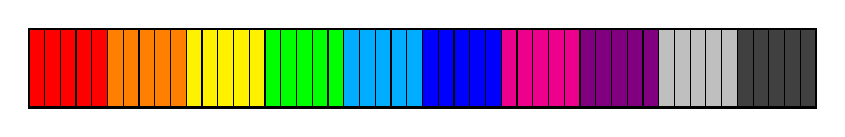
\begin{tikzpicture}
  \filldraw[fill=red]    (0, 0) rectangle  +(1,1);
  \filldraw[fill=orange] (1, 0) rectangle  +(1,1);
  \filldraw[fill=yellow] (2, 0) rectangle  +(1,1);
  \filldraw[fill=green]  (3, 0) rectangle  +(1,1);
  \filldraw[fill=cyan]   (4, 0) rectangle  +(1,1);
  \filldraw[fill=blue]   (5, 0) rectangle  +(1,1);
  \filldraw[fill=magenta] (6, 0) rectangle  +(1,1);
  \filldraw[fill=violet] (7, 0) rectangle +(1,1);
  \filldraw[fill=lightgray] (8, 0) rectangle +(1,1);
  \filldraw[fill=darkgray] (9, 0) rectangle +(1,1);
  
  \draw[thick] (0, 0) rectangle (10, 1);
  \foreach \i in {0.2, 0.4, ..., 9.8}
  \draw (\i, 0) -- +(0, 1);
\end{tikzpicture}

\begin{itemize}
\item Easiest !
\item Favored by MPI
\end{itemize}

\vspace{1cm}

Cyclic

\medskip

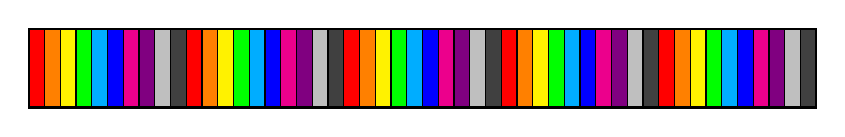
\begin{tikzpicture}
  \foreach \i in {0, 2, 4, 6, 8} {
    \filldraw[fill=red]    (\i, 0) rectangle  +(0.2,1);
    \filldraw[fill=orange]    (\i + 0.2, 0) rectangle  +(0.2,1);
    \filldraw[fill=yellow]    (\i + 0.4, 0) rectangle  +(0.2,1);
    \filldraw[fill=green]    (\i + 0.6, 0) rectangle  +(0.2,1);
    \filldraw[fill=cyan]    (\i + 0.8, 0) rectangle  +(0.2,1);
    \filldraw[fill=blue]    (\i + 1, 0) rectangle  +(0.2,1);
    \filldraw[fill=magenta]    (\i + 1.2, 0) rectangle  +(0.2,1);
    \filldraw[fill=violet]    (\i + 1.4, 0) rectangle  +(0.2,1);
    \filldraw[fill=lightgray]    (\i + 1.6, 0) rectangle  +(0.2,1);
    \filldraw[fill=darkgray]    (\i + 1.8, 0) rectangle  +(0.2,1);
  }
  % \filldraw[fill=red]    (0, 0) rectangle  +(1,1);
  % \filldraw[fill=orange] (1, 0) rectangle  +(1,1);
  % \filldraw[fill=yellow] (2, 0) rectangle  +(1,1);
  % \filldraw[fill=green]  (3, 0) rectangle  +(1,1);
  % \filldraw[fill=cyan]   (4, 0) rectangle  +(1,1);
  % \filldraw[fill=blue]   (5, 0) rectangle  +(1,1);
  % \filldraw[fill=magenta] (6, 0) rectangle  +(1,1);
  % \filldraw[fill=violet] (7, 0) rectangle +(1,1);
  % \filldraw[fill=lightgray] (8, 0) rectangle +(1,1);
  % \filldraw[fill=darkgray] (9, 0) rectangle +(1,1);
  
  \draw[thick] (0, 0) rectangle (10, 1);
  \foreach \i in {0.2, 0.4, ..., 9.8}
  \draw (\i, 0) -- +(0, 1);
\end{tikzpicture}

\begin{itemize}
\item May improve load balancing
\item Also possible with MPI
  \begin{itemize}
  \item Must create ``types'' $\leadsto$ \mintinline{C}{MPI_Type_vector}...
  \end{itemize}
\end{itemize}
\end{frame}

%%%%%%%%%%%%%%%%%%%%%%%%%%%%%%%%%%%%%%%%%%%%%%%%%%%%

\begin{frame}
\frametitle{1D Distribution of 2D Data}

By blocs:

\medskip

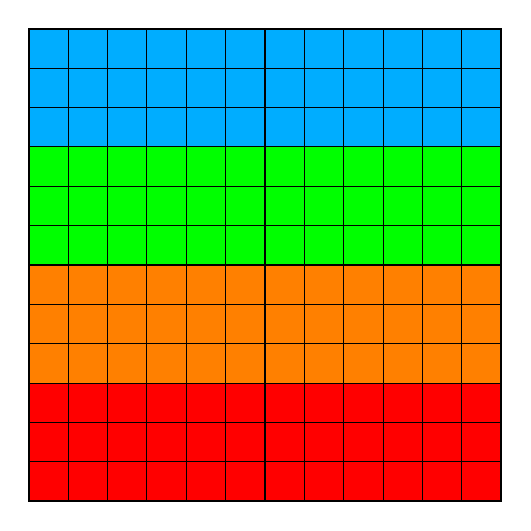
\begin{tikzpicture}[scale=0.5]
  \filldraw[fill=red]    (0, 0) rectangle  +(12,3);
  \filldraw[fill=orange] (0, 3) rectangle  +(12,3);
  \filldraw[fill=green] (0, 6) rectangle  +(12,3);
  \filldraw[fill=cyan]  (0, 9) rectangle  +(12,3);
  
  \draw[thick] (0, 0) rectangle (12, 12);
  \foreach \i in {1, 2, ..., 11} {
    \draw (\i, 0) -- +(0, 12);
    \draw (0, \i) -- +(12, 0);
  }
\end{tikzpicture}
\end{frame}


%%%%%%%%%%%%%%%%%%%%%%%%%%%%%%%%%%%%%%%%%%%%%%%%%%%%

\begin{frame}
\frametitle{1D Distribution of 2D Data}

Cyclic:

\medskip

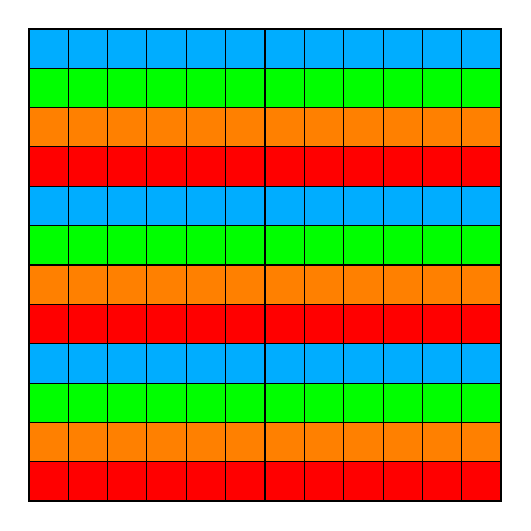
\begin{tikzpicture}[scale=0.5]
  \foreach \i in {0, 4, 8} {
    \filldraw[fill=red]    (0, \i) rectangle  +(12,1);
    \filldraw[fill=orange] (0, 1+\i) rectangle  +(12,1);
    \filldraw[fill=green] (0, 2+\i) rectangle  +(12,1);
    \filldraw[fill=cyan]  (0, 3+\i) rectangle  +(12,1);
  }
  \draw[thick] (0, 0) rectangle (12, 12);
  \foreach \i in {1, 2, ..., 11} {
    \draw (\i, 0) -- +(0, 12);
    \draw (0, \i) -- +(12, 0);
  }
\end{tikzpicture}
\end{frame}

%%%%%%%%%%%%%%%%%%%%%%%%%%%%%%%%

\begin{frame}
\frametitle{2D Distribution of 2D Data}

By blocs:

\medskip

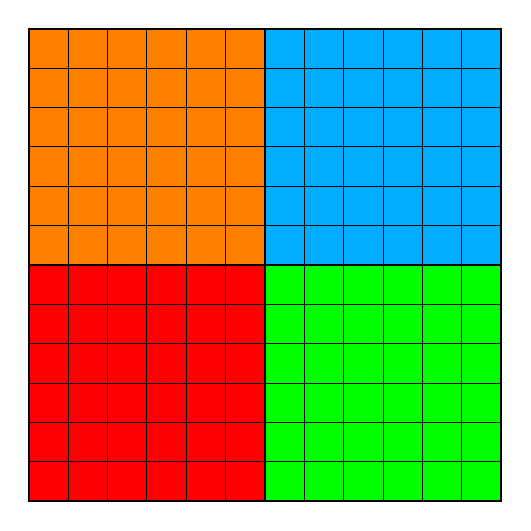
\begin{tikzpicture}[scale=0.5]
  \filldraw[fill=red]    (0, 0) rectangle  +(6, 6);
  \filldraw[fill=orange] (0, 6) rectangle  +(6,6);
  \filldraw[fill=green] (6, 0) rectangle  +(6,6);
  \filldraw[fill=cyan]  (6, 6) rectangle  +(6,6);

  \draw[thick] (0, 0) rectangle (12, 12);
  \foreach \i in {1, 2, ..., 11} {
    \draw (\i, 0) -- +(0, 12);
    \draw (0, \i) -- +(12, 0);
  }
\end{tikzpicture}
\end{frame}

%%%%%%%%%%

\begin{frame}
\frametitle{2D Distribution of 2D Data}

Cyclic:

\medskip

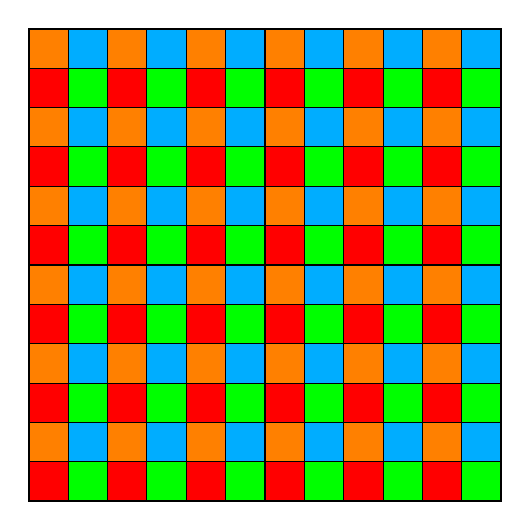
\begin{tikzpicture}[scale=0.5]
  \foreach \i in {0, 2, 4, 6, 8, 10} {
    \foreach \j in {0, 2, 4, 6, 8, 10} {
      \filldraw[fill=red]    (\i, \j) rectangle  +(1, 1);
      \filldraw[fill=orange] (\i, 1+\j) rectangle  +(1,1);
      \filldraw[fill=green] (\i+1, \j) rectangle  +(1,1);
      \filldraw[fill=cyan]  (\i+1, 1+\j) rectangle  +(1,1);
    }
  }
  \draw[thick] (0, 0) rectangle (12, 12);
  \foreach \i in {1, 2, ..., 11} {
    \draw (\i, 0) -- +(0, 12);
    \draw (0, \i) -- +(12, 0);
  }
\end{tikzpicture}
\end{frame}

%%%%%%%%%%%%%%%%%%%%%%%%%%%%%%%%%%%%%%%%%%%%%%%%%%%%%%%%%%%%%%

\begin{frame}
\frametitle{2D Distribution of 2D Data}

Block-Cyclic:

\medskip

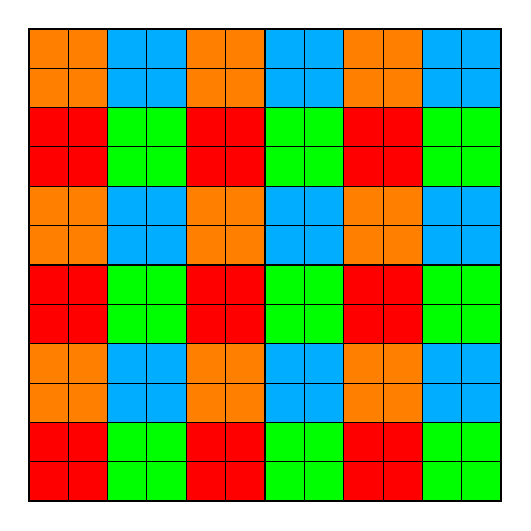
\begin{tikzpicture}[scale=0.5]
  \foreach \i in {0, 4, 8} {
    \foreach \j in {0, 4, 8} {
      \filldraw[fill=red]    (\i, \j) rectangle  +(2, 2);
      \filldraw[fill=orange] (\i, 2+\j) rectangle  +(2,2);
      \filldraw[fill=green] (\i+2, \j) rectangle  +(2,2);
      \filldraw[fill=cyan]  (\i+2, 2+\j) rectangle  +(2,2);
    }
  }
  \draw[thick] (0, 0) rectangle (12, 12);
  \foreach \i in {1, 2, ..., 11} {
    \draw (\i, 0) -- +(0, 12);
    \draw (0, \i) -- +(12, 0);
  }
\end{tikzpicture}
\end{frame}


%%%%%%%%%%%%%%%%%%%%%%%%%%%%%%%%%%%%%%%%%%%%%%%%%%%%%%%%%%%%%%

\begin{frame}
\frametitle{1D Distribution of 3D Data}

\centering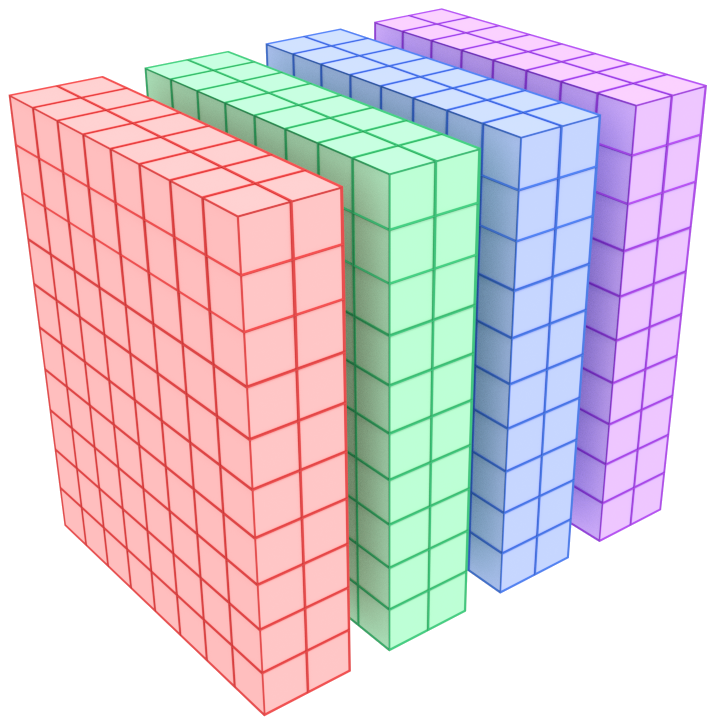
\includegraphics[height=8cm]{slabs.png}

\end{frame}

%%%%%%%%%%%%%%%%%%%%%%%%

\begin{frame}
\frametitle{2D Distribution of 3D Data}

\centering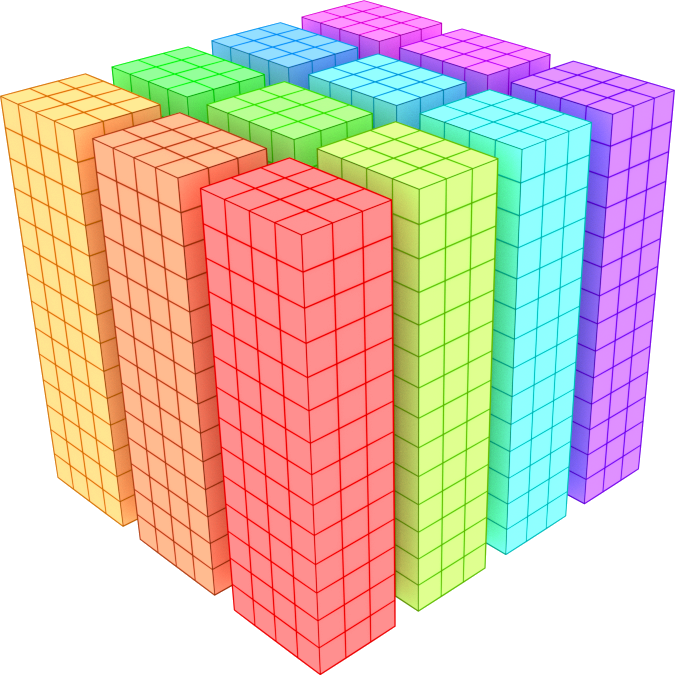
\includegraphics[height=8cm]{pencils.png}

\end{frame}

%%%%%%%%%%%%%%%%%%%%%%%%%

\begin{frame}[fragile=singleslide]
\frametitle{Data Parallelism (continued)}


\begin{block}{Classic example: \emph{reduce}}
\begin{minted}{C}
sum = 0
for (int i = 0; i < n; i++)
    sum = sum + A[i]
\end{minted}
\end{block}

\bigskip

\begin{itemize}
\item Data dependency on \mintinline{C}{sum}? Easy to bypass
\item Distributed memory $\rightarrow$ communications
\item Binomial tree algorithm
\end{itemize}
\end{frame}

%%%%%%%%%%%%%%%%%%%%%%%%%%%%%%%%%%%%%%%%%%%%%%%%%%%%%%%%%%%%%%%%

\begin{frame}[fragile=singleslide]
  \frametitle{MPI in action: \texttt{reduce}}

  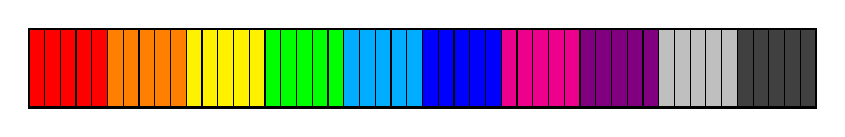
\begin{tikzpicture}
    \filldraw[fill=red]    (0, 0) rectangle  +(1,1);
    \filldraw[fill=orange] (1, 0) rectangle  +(1,1);
    \filldraw[fill=yellow] (2, 0) rectangle  +(1,1);
    \filldraw[fill=green]  (3, 0) rectangle  +(1,1);
    \filldraw[fill=cyan]   (4, 0) rectangle  +(1,1);
    \filldraw[fill=blue]   (5, 0) rectangle  +(1,1);
    \filldraw[fill=magenta] (6, 0) rectangle  +(1,1);
    \filldraw[fill=violet] (7, 0) rectangle +(1,1);
    \filldraw[fill=lightgray] (8, 0) rectangle +(1,1);
    \filldraw[fill=darkgray] (9, 0) rectangle +(1,1);
    \draw[thick] (0, 0) rectangle (10, 1);
    \foreach \i in {0.2, 0.4, ..., 9.8}
    \draw (\i, 0) -- +(0, 1);
  \end{tikzpicture}
  
  \bigskip

\begin{minted}[fontsize=\small]{C}
// Global array of size n
// p processes
int root = 0;
double sum = 0;
for (int i = rank * n / p; (rank + 1) * n / p; i++)
        sum += A[i];
MPI_Reduce(MPI_IN_PLACE, &sum, 1, MPI_DOUBLE, MPI_SUM,
           root, MPI_COMM_WORLD);
\end{minted}        

\begin{align*}
  T &= \frac{n}{p} + \lceil \log_2 p \rceil (\alpha + \beta)
\end{align*}
\end{frame}

%%%%%%%%%%%%%%%%%%%%%%%%%%%%%%%%%%%%%%%%%%%%%%%%%%%%%

% \begin{frame}
% \frametitle{\alert{Shared}-memory \texttt{reduce}}

% \begin{tikzpicture}
%   \filldraw[fill=red]    (0, 0) rectangle  +(1,1);
%   \filldraw[fill=orange] (1, 0) rectangle  +(1,1);
%   \filldraw[fill=yellow] (2, 0) rectangle  +(1,1);
%   \filldraw[fill=green]  (3, 0) rectangle  +(1,1);
%   \filldraw[fill=cyan]   (4, 0) rectangle  +(1,1);
%   \filldraw[fill=blue]   (5, 0) rectangle  +(1,1);
%   \filldraw[fill=magenta] (6, 0) rectangle  +(1,1);
%   \filldraw[fill=violet] (7, 0) rectangle +(1,1);
%   \filldraw[fill=lightgray] (8, 0) rectangle +(1,1);
%   \filldraw[fill=darkgray] (9, 0) rectangle +(1,1);
  
%   \draw[thick] (0, 0) rectangle (10, 1);
%   \foreach \i in {0.2, 0.4, ..., 9.8}
%   \draw (\i, 0) -- +(0, 1);
% \end{tikzpicture}

% \bigskip

% \begin{enumerate}
% \item Tableau \texttt{Scratch} de taille $p$.
% \item $P_i$ fait : $\texttt{Scratch[i]} \gets $ somme de \emph{ses} donnée.
% \item \alert{Barrière}
% \item $P_0$ calcule la somme de \texttt{Scratch} puis l'écrit dans \texttt{sum}
% \item \alert{Barrière}
% \end{enumerate}


% \begin{align*}
%   T &= \frac{n}{p} + p \\
%     &\geq 2 \sqrt{n} & \text{(optimal atteint avec $\sqrt{n}$ processeurs)}
% \end{align*}
% \end{frame}

% %%%%%%%%%%%%%%%%%%%%%%%%%%%%%%%%%%%%%%%%%%%%%%%%%%%%%%%%%%%%%%%%

% \begin{frame}
% \frametitle{Algorithme (mémoire partagée) pour \texttt{reduce}}

% \begin{tikzpicture}
%   \filldraw[fill=red]    (0, 0) rectangle  +(1,1);
%   \filldraw[fill=orange] (1, 0) rectangle  +(1,1);
%   \filldraw[fill=yellow] (2, 0) rectangle  +(1,1);
%   \filldraw[fill=green]  (3, 0) rectangle  +(1,1);
%   \filldraw[fill=cyan]   (4, 0) rectangle  +(1,1);
%   \filldraw[fill=blue]   (5, 0) rectangle  +(1,1);
%   \filldraw[fill=magenta] (6, 0) rectangle  +(1,1);
%   \filldraw[fill=violet] (7, 0) rectangle +(1,1);
%   \filldraw[fill=lightgray] (8, 0) rectangle +(1,1);
%   \filldraw[fill=darkgray] (9, 0) rectangle +(1,1);
  
%   \draw[thick] (0, 0) rectangle (10, 1);
%   \foreach \i in {0.2, 0.4, ..., 9.8}
%   \draw (\i, 0) -- +(0, 1);
% \end{tikzpicture}

% \bigskip

% \begin{block}{$\texttt{reduce}(A, n):$}
%   \begin{enumerate}
%   \item Si $n = 1$, renvoyer $A[0]$.
%   \item Allouer un tableau \texttt{Scratch} de taille $n/2$.
%   \item Pour tout $0 \leq i < n/2$, faire (en parallèle):
%     \begin{itemize}
%     \item $\texttt{Scratch}[i] \gets A[2i] + A[2i+1]$.  
%     \end{itemize}
    
%   \item renvoyer : $\texttt{reduce}(\texttt{Scratch}, n/2)$.
%   \end{enumerate}
% \end{block}

% \begin{align*}
%   T &= \frac{2n}{p} + \log_2 p \\
%     &\geq 1 + \log_2 p & \text{(optimal atteint avec $n/2$ processeurs)}
% \end{align*}
% \end{frame}

\section{EDPs}

%%%%%%%%%%%%%%%%%%%%%%%%%%%%%%%%%%%%%%%%%%%%%%%%%%%%%%%%%%%%%%%%%%%%%

\begin{frame}
\frametitle{Approximating Solutions of PDEs}

\begin{block}{Classic example: heat equation}
  \[
    \frac{\partial T}{\partial t} = \alpha \nabla^2 T = \alpha \left( \frac{\partial^2 T}{\partial x^2} + \frac{\partial^2 T}{\partial y^2} + \frac{\partial^2 T}{\partial z^2}\right)
  \]
  
  \begin{itemize}
  \item Heat diffusion in homogeneous material
  \item $T(x,y,z,t) = $ temperature in point $(x,y,z)$ at time $t$
  \end{itemize}
\end{block}

\medskip
\begin{alertblock}{Goal :}
\begin{itemize}
\item Compute $T(x, y, z, t)$
\item Over a finite domain
\item $T(x, y, z, 0)$ known (initial conditions)
\item Eventual boundary conditions (e.g. $T(0, y, z, t) = cst$)
\end{itemize}
\end{alertblock}
\end{frame}

%%%%%%%%%%%%%%%%%%%%%%%%%%%%%%%%%%%%%%%%%%%%%%%%%%%%%%%%%%%%%%%%%%%%%

\begin{frame}
\frametitle{Approximating Solutions of PDEs}
\framesubtitle{Euler's Method}

  \[
    \frac{\partial T}{\partial t} = \alpha \nabla^2 T = \alpha \left( \frac{\partial^2 T}{\partial x^2} + \frac{\partial^2 T}{\partial y^2} + \frac{\partial^2 T}{\partial z^2}\right)
  \]

  \begin{exampleblock}{Approximation}
    \begin{itemize}
    \item Divide time in small intervals
      \[
        \frac{\partial T}{\partial t} \approx \frac{T(x,y, t + \Delta t) - T(x,y, t)}{\Delta t}
      \]
    \item Divide space in small ``cells''
    \end{itemize}
    \[
      \frac{\partial^2 T}{\partial x^2} \approx \frac{T(x - \Delta x,y,t) - 2 T(x,y,t) + T(x + \Delta x,y,t)}{ \Delta x^2 }
    \]
  \end{exampleblock}
\end{frame}

%%%%%%%%%%%%%%%%%%%%%%%%%%%%%%%%%%%%%%%%%%%%%%%%%%%%%%%%%%%%%%%%%%%%%

\begin{frame}
\frametitle{Approximating Solutions of PDEs}
\framesubtitle{Euler's Method}

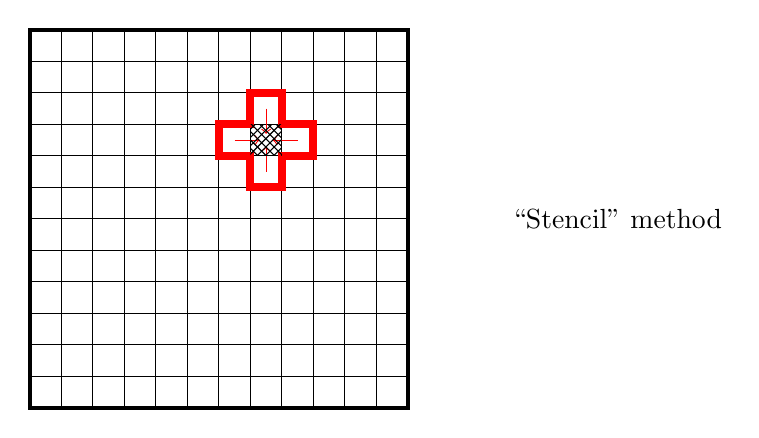
\begin{tikzpicture}[scale=0.4]
  \draw[ultra thick] (0, 0) rectangle (12, 12);
  \foreach \i in {1, 2, ..., 11} {
    \draw (\i, 0) -- +(0, 12);
    \draw (0, \i) -- +(12, 0);
  }

  \only<2>{
  \begin{scope}[xshift=2cm, yshift=2cm]
    % "croix" qui dépasse
    \draw[red, line width=1mm] (5, 5) -- ++(0, 1) -- ++ (-1, 0) -- ++(0, 1) --
    ++(1, 0) -- ++(0, 1) -- ++(1, 0) -- ++(0, -1) -- ++(1, 0) -- ++(0, -1) --
    ++(-1, 0) -- ++(0, -1) -- cycle;
    % petites flèches
    \draw[red,->] (5.5, 5.5) -- +(0, 0.8);
    \draw[red,->] (5.5, 7.5) -- +(0, -0.8);
    \draw[red,->] (4.5, 6.5) -- +(0.8, 0);
    \draw[red,->] (6.5, 6.5) -- +(-0.8, 0);
    \end{scope}
  }
    \fill<3>[pattern=crosshatch] (7, 8) rectangle +(1, 1);

    \node[anchor=west] at (15, 6) {``Stencil'' method};
  \end{tikzpicture}


\end{frame}

%%%%%%%%%%%%%%%%%%%%%%%%%%%%%%%%%%%%%%%%%%%%%%%%%%%%%%%%%%%%%%%%%%%%%%

\begin{frame}
\frametitle{``Domain Decomposition'' (a.k.a. Data Parallelism)}


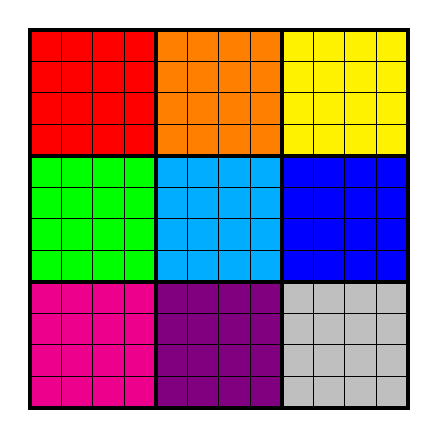
\begin{tikzpicture}[scale=0.4]
  \filldraw[very thick, fill=red]       (0, 8) rectangle  +(4, 4);
  \filldraw[very thick, fill=orange]    (4, 8) rectangle  +(4,4);
  \filldraw[very thick, fill=yellow]    (8, 8) rectangle  +(4,4);
  \filldraw[very thick, fill=green]     (0, 4) rectangle  +(4,4);
  \filldraw[very thick, fill=cyan]      (4, 4) rectangle  +(4,4);
  \filldraw[very thick, fill=blue]      (8, 4) rectangle  +(4,4);
  \filldraw[very thick, fill=magenta]   (0, 0) rectangle  +(4,4);
  \filldraw[very thick, fill=violet]    (4, 0) rectangle  +(4,4);
  \filldraw[very thick, fill=lightgray] (8, 0) rectangle  +(4,4);

  
  \draw[ultra thick] (0, 0) rectangle (12, 12);
  \foreach \i in {1, 2, ..., 11} {
    \draw (\i, 0) -- +(0, 12);
    \draw (0, \i) -- +(12, 0);
  }

  
  \end{tikzpicture}
\end{frame}

%%%%%%%%%%%%%%%%%%%%%%%%%%%%%%%%%%%%%%%%%%%%%%%%%%%%%%%%%%%%%%%%%%%%%%%%%%


\begin{frame}
\frametitle{``Domain Decomposition'' (a.k.a. Data Parallelism)}


\begin{tikzpicture}[scale=0.4]
  \path[use as bounding box] (1, 0) rectangle (18, 18);
  
  % gros carrés
  \filldraw[very thick, fill=red]       (0,  14) rectangle  +(4, 4);
  \filldraw[very thick, fill=orange]    (7,  14) rectangle  +(4,4);
  \filldraw[very thick, fill=yellow]    (14, 14) rectangle  +(4,4);
  \filldraw[very thick, fill=green]     (0,  7) rectangle  +(4,4);
  \filldraw[very thick, fill=cyan]      (7,  7) rectangle  +(4,4);
  \filldraw[very thick, fill=blue]      (14, 7) rectangle  +(4,4);
  \filldraw[very thick, fill=magenta]   (0,  0) rectangle  +(4,4);
  \filldraw[very thick, fill=violet]    (7,  0) rectangle  +(4,4);
  \filldraw[very thick, fill=lightgray] (14, 0) rectangle  +(4,4);
  
  % petites cases
  \foreach \i in {0, 1, 2} {
    \foreach \j in {0, 1, 2} {
      \foreach \k in {1, 2, 3} {
        \draw (7*\i + \k, 7*\j) -- +(0, 4);
        \draw (7*\i, 7*\j + \k) -- +(4, 0);
      }
    }
  }

  \fill<4->[pattern=crosshatch] (9, 8) rectangle +(1, 1);
  \fill<3->[pattern=crosshatch] (8, 8) rectangle +(1, 1);
  
  \begin{onlyenv}<4>
      \begin{scope}[xshift=5cm, yshift=2cm]
      % "croix" qui dépasse
      \draw[red, line width=1mm] (5, 5) -- ++(0, 1) -- ++ (-1, 0) -- ++(0, 1) --
      ++(1, 0) -- ++(0, 1) -- ++(1, 0) -- ++(0, -1) -- ++(1, 0) -- ++(0, -1) --
      ++(-1, 0) -- ++(0, -1) -- cycle;
      % petites flèches
      \draw[red,->] (5.5, 5.5) -- +(0, 0.8);
      \draw[red,->] (5.5, 7.5) -- +(0, -0.8);
      \draw[red,->] (4.5, 6.5) -- +(0.8, 0);
      \draw[red,->] (6.5, 6.5) -- +(-0.8, 0);
    \end{scope}
  \end{onlyenv}
  
  \begin{onlyenv}<3>
    \begin{scope}[xshift=4cm, yshift=2cm]
      % "croix"
      \draw[red, line width=1mm] (5, 5) -- ++(0, 1) -- ++ (-1, 0) -- ++(0, 1) --
      ++(1, 0) -- ++(0, 1) -- ++(1, 0) -- ++(0, -1) -- ++(1, 0) -- ++(0, -1) --
      ++(-1, 0) -- ++(0, -1) -- cycle;
      % petites flèches
      \draw[red,->] (5.5, 5.5) -- +(0, 0.8);
      \draw[red,->] (5.5, 7.5) -- +(0, -0.8);
      \draw[red,->] (4.5, 6.5) -- +(0.8, 0);
      \draw[red,->] (6.5, 6.5) -- +(-0.8, 0);
    \end{scope}
  \end{onlyenv}
  
  \begin{onlyenv}<2>
    \begin{scope}[xshift=3cm, yshift=2cm]
      % "croix"
      \draw[red, line width=1mm] (5, 5) -- ++(0, 1) -- ++ (-1, 0) -- ++(0, 1) --
      ++(1, 0) -- ++(0, 1) -- ++(1, 0) -- ++(0, -1) -- ++(1, 0) -- ++(0, -1) --
      ++(-1, 0) -- ++(0, -1) -- cycle;
      % petites flèches
      \draw[red,->] (5.5, 5.5) -- +(0, 0.8);
      \draw[red,->] (5.5, 7.5) -- +(0, -0.8);
      \draw[red,->] (4.5, 6.5) -- +(0.8, 0);
      \draw[red,->] (6.5, 6.5) -- +(-0.8, 0);
    \end{scope}
  \end{onlyenv}
  
  \filldraw<5>[fill=blue] (11, 7) rectangle  +(1,4);
  \draw<5> (11, 8) --  +(1,0);
  \draw<5> (11, 9) --  +(1,0);
  \draw<5> (11, 10) --  +(1,0);
  \draw<5> (11, 8) --  +(1,0);
  \draw<5>[very thick]      (7,  7) rectangle  +(5,4);  
\end{tikzpicture}
\end{frame}


%%%%%%%%%%%%%%%%%%%%%%%%%%%%%%%%%%%%%%%%%%%%%%%%%%%%%%%%%%%%%%%%%%%%%%%%%%

\begin{frame}
\frametitle{``Domain Decomposition'' (a.k.a. Data Parallelism)}

\begin{minipage}[T]{7.2cm}
\begin{tikzpicture}[scale=0.4]
  \path[use as bounding box] (1, 0) rectangle (18, 18);
  
  % halos
  \begin{onlyenv}<3->
  \filldraw[fill=violet]    (4, 0) rectangle  +(1,4);
  \filldraw[fill=magenta]   (6, 0) rectangle  +(1,4);
  \filldraw[fill=lightgray] (11, 0) rectangle  +(1,4);
  \filldraw[fill=violet]    (13, 0) rectangle  +(1,4);
  \filldraw[fill=cyan]    (4, 7) rectangle  +(1,4);
  \filldraw[fill=green]   (6, 7) rectangle  +(1,4);
  \filldraw[fill=blue] (11, 7) rectangle  +(1,4);
  \filldraw[fill=cyan]    (13, 7) rectangle  +(1,4);
  \filldraw[fill=orange]    (4, 14) rectangle  +(1,4);
  \filldraw[fill=red]   (6, 14) rectangle  +(1,4);
  \filldraw[fill=yellow]    (11,14) rectangle  +(1,4);
  \filldraw[fill=orange]    (13,14) rectangle  +(1,4);
  
  \filldraw[fill=blue]      (14, 4) rectangle  +(4,1);
  \filldraw[fill=cyan]      (7, 4) rectangle  +(4,1);
  \filldraw[fill=green]      (0, 4) rectangle  +(4,1);
  \filldraw[fill=lightgray]   (14, 6) rectangle  +(4,1);
  \filldraw[fill=violet]      (7, 6) rectangle  +(4,1);
  \filldraw[fill=magenta]     (0, 6) rectangle  +(4,1);  
  \filldraw[fill=blue]      (14, 13) rectangle  +(4,1);
  \filldraw[fill=cyan]      (7, 13) rectangle  +(4,1);
  \filldraw[fill=green]      (0, 13) rectangle  +(4,1);
  \filldraw[fill=yellow]      (14, 11) rectangle  +(4,1);
  \filldraw[fill=orange]      (7, 11) rectangle  +(4,1);
  \filldraw[fill=red]      (0, 11) rectangle  +(4,1);
\end{onlyenv}

  % gros carrés
    \filldraw[very thick, fill=red]       (0,  14) rectangle  +(4, 4);
    \filldraw[very thick, fill=orange]    (7,  14) rectangle  +(4,4);
    \filldraw[very thick, fill=yellow]    (14, 14) rectangle  +(4,4);
    \filldraw[very thick, fill=green]     (0,  7) rectangle  +(4,4);
    \filldraw[very thick, fill=cyan]      (7,  7) rectangle  +(4,4);
    \filldraw[very thick, fill=blue]      (14, 7) rectangle  +(4,4);
    \filldraw[very thick, fill=magenta]   (0,  0) rectangle  +(4,4);
    \filldraw[very thick, fill=violet]    (7,  0) rectangle  +(4,4);
    \filldraw[very thick, fill=lightgray] (14, 0) rectangle  +(4,4);
  
  \begin{onlyenv}<4->
    \draw[pattern=crosshatch, pattern color=black, very thick]       (0,  14) rectangle  +(4, 4);
    \draw[pattern=crosshatch, pattern color=black, very thick]    (7,  14) rectangle  +(4,4);
    \draw[pattern=crosshatch, pattern color=black, very thick]    (14, 14) rectangle  +(4,4);
    \draw[pattern=crosshatch, pattern color=black, very thick]     (0,  7) rectangle  +(4,4);
    \draw[pattern=crosshatch, pattern color=black, very thick]      (7,  7) rectangle  +(4,4);
    \draw[pattern=crosshatch, pattern color=black, very thick]      (14, 7) rectangle  +(4,4);
    \draw[pattern=crosshatch, pattern color=black, very thick]   (0,  0) rectangle  +(4,4);
    \draw[pattern=crosshatch, pattern color=black, very thick]    (7,  0) rectangle  +(4,4);
    \draw[pattern=crosshatch, pattern color=black, very thick] (14, 0) rectangle  +(4,4);
  \end{onlyenv}
  
  % hachures

  % petites cases, sans halo
  \begin{onlyenv}<1-2>
    \foreach \i in {0, 1, 2} {
      \foreach \j in {0, 1, 2} {
        \foreach \k in {1, 2, 3} {
          \draw (7*\i + \k, 7*\j) -- +(0, 4);
          \draw (7*\i, 7*\j + \k) -- +(4, 0);
        }
      }
    }
  \end{onlyenv}

  \begin{onlyenv}<3->
  % petites cases, halos compris
  \foreach \k in {1, 2, 3} {
    \draw (\k, 0) -- +(0, 5);
    \draw (0, \k) -- +(5, 0);
  }
  \foreach \k in {1, 2, 3} {
    \draw (\k, 6) -- +(0, 6);
    \draw (0, 7 + \k) -- +(5, 0);
  }
  \foreach \k in {1, 2, 3, 4} {
    \draw (\k, 13) -- +(0, 5);
    \draw (0, 13 + \k) -- +(5, 0);
  }
  \foreach \k in {1, 2, 3} {
    \draw (7 + \k, 0) -- +(0, 5);
    \draw (6, \k) -- +(6, 0);
  }
  \foreach \k in {1, 2, 3} {
    \draw (7 + \k, 6) -- +(0, 6);
    \draw (6, 7 + \k) -- +(6, 0);
  }
  \foreach \k in {1, 2, 3} {
    \draw (7 + \k, 13) -- +(0, 5);
    \draw (6, 14 + \k) -- +(6, 0);
  }
  \foreach \k in {1, 2, 3} {
    \draw (14 + \k, 0) -- +(0, 5);
    \draw (13, \k) -- +(5, 0);
  }
  \foreach \k in {1, 2, 3} {
    \draw (14 + \k, 6) -- +(0, 6);
    \draw (13, 7 + \k) -- +(5, 0);
  }
  \foreach \k in {1, 2, 3} {
    \draw (14 + \k, 13) -- +(0, 5);
    \draw (13, 14 + \k) -- +(5, 0);
  }
\end{onlyenv}

% flèches des halos
  \begin{onlyenv}<2,5>
 \begin{scope}[xshift=0cm, yshift=14cm]
   \draw[red, ultra thick, ->] (3.5, 0) to[bend right=20mm] +(2.5, 0);
   \draw[red, ultra thick, ->] (0, 0.5) to[bend right=20mm] +(0, -2.5);
 \end{scope}
 \begin{scope}[xshift=7cm, yshift=14cm]
   \draw[orange, ultra thick, ->] (3.5, 0) to[bend right=20mm] +(2.5, 0);
   \draw[orange, ultra thick, ->] (0.5, 4) to[bend right=20mm] +(-2.5, 0);
   \draw[orange, ultra thick, ->] (0, 0.5) to[bend right=20mm] +(0, -2.5);
 \end{scope}
 \begin{scope}[xshift=14cm, yshift=14cm]
   \draw[yellow, ultra thick, ->] (0.5, 4) to[bend right=20mm] +(-2.5, 0);
   \draw[yellow, ultra thick, ->] (0, 0.5) to[bend right=20mm] +(0, -2.5);
 \end{scope}

 \begin{scope}[xshift=0cm, yshift=7cm]
 \draw[green, ultra thick, ->] (3.5, 0) to[bend right=20mm] +(2.5, 0);
 \draw[green, ultra thick, ->] (0, 0.5) to[bend right=20mm] +(0, -2.5);
 \draw[green, ultra thick, ->] (4, 3.5) to[bend right=20mm] +(0, 2.5);
\end{scope}
 \begin{scope}[xshift=7cm, yshift=7cm]
 \draw[cyan, ultra thick, ->] (3.5, 0) to[bend right=20mm] +(2.5, 0);
 \draw[cyan, ultra thick, ->] (0.5, 4) to[bend right=20mm] +(-2.5, 0);
 \draw[cyan, ultra thick, ->] (0, 0.5) to[bend right=20mm] +(0, -2.5);
 \draw[cyan, ultra thick, ->] (4, 3.5) to[bend right=20mm] +(0, 2.5);
\end{scope}
  \begin{scope}[xshift=14cm, yshift=7cm]
 \draw[blue, ultra thick, ->] (0.5, 4) to[bend right=20mm] +(-2.5, 0);
 \draw[blue, ultra thick, ->] (0, 0.5) to[bend right=20mm] +(0, -2.5);
 \draw[blue, ultra thick, ->] (4, 3.5) to[bend right=20mm] +(0, 2.5);
\end{scope}
 \begin{scope}[xshift=0cm, yshift=0cm]
 \draw[magenta, ultra thick, ->] (3.5, 0) to[bend right=20mm] +(2.5, 0);
 \draw[magenta, ultra thick, ->] (4, 3.5) to[bend right=20mm] +(0, 2.5);
\end{scope}
 \begin{scope}[xshift=7cm, yshift=0cm]
 \draw[violet, ultra thick, ->] (3.5, 0) to[bend right=20mm] +(2.5, 0);
 \draw[violet, ultra thick, ->] (0.5, 4) to[bend right=20mm] +(-2.5, 0);
 \draw[violet, ultra thick, ->] (4, 3.5) to[bend right=20mm] +(0, 2.5);
\end{scope}
  \begin{scope}[xshift=14cm, yshift=0cm]
 \draw[lightgray, ultra thick, ->] (0.5, 4) to[bend right=20mm] +(-2.5, 0);
 \draw[lightgray, ultra thick, ->] (4, 3.5) to[bend right=20mm] +(0, 2.5);
\end{scope}
\end{onlyenv}

\end{tikzpicture}%
\end{minipage}\begin{minipage}[T]{4.5cm}
  Each processor:
  \medskip
  \begin{itemize}
  \item<1-> Knows $T$ at time~$t$
  \item<2-> Sends/Receives the \alert{halo} from its neighbors
  \item<4-> Compute $T$ at time $t + \Delta t$
  \item<5-> Rinse, repeat
  \end{itemize}

  \medskip

  \begin{alertblock}<6>{Problem}
    Progress blocked by communications
  \end{alertblock}
\end{minipage}
\end{frame}


%%%%%%%%%%%%%%%%%%%%%%%%%%%%%%%%%%%%%%%%

\begin{frame}
\frametitle{``Domain Decomposition'' (a.k.a. Data Parallelism)}

\begin{minipage}[T]{7.2cm}
\begin{tikzpicture}[scale=0.4]
  \path[use as bounding box] (1, 0) rectangle (18, 18);
  
  % halos
  \begin{onlyenv}<4->
  \filldraw[fill=violet]    (4, 0) rectangle  +(1,4);
  \filldraw[fill=magenta]   (6, 0) rectangle  +(1,4);
  \filldraw[fill=lightgray] (11, 0) rectangle  +(1,4);
  \filldraw[fill=violet]    (13, 0) rectangle  +(1,4);
  \filldraw[fill=cyan]    (4, 7) rectangle  +(1,4);
  \filldraw[fill=green]   (6, 7) rectangle  +(1,4);
  \filldraw[fill=blue] (11, 7) rectangle  +(1,4);
  \filldraw[fill=cyan]    (13, 7) rectangle  +(1,4);
  \filldraw[fill=orange]    (4, 14) rectangle  +(1,4);
  \filldraw[fill=red]   (6, 14) rectangle  +(1,4);
  \filldraw[fill=yellow]    (11,14) rectangle  +(1,4);
  \filldraw[fill=orange]    (13,14) rectangle  +(1,4);
  
  \filldraw[fill=blue]      (14, 4) rectangle  +(4,1);
  \filldraw[fill=cyan]      (7, 4) rectangle  +(4,1);
  \filldraw[fill=green]      (0, 4) rectangle  +(4,1);
  \filldraw[fill=lightgray]   (14, 6) rectangle  +(4,1);
  \filldraw[fill=violet]      (7, 6) rectangle  +(4,1);
  \filldraw[fill=magenta]     (0, 6) rectangle  +(4,1);  
  \filldraw[fill=blue]      (14, 13) rectangle  +(4,1);
  \filldraw[fill=cyan]      (7, 13) rectangle  +(4,1);
  \filldraw[fill=green]      (0, 13) rectangle  +(4,1);
  \filldraw[fill=yellow]      (14, 11) rectangle  +(4,1);
  \filldraw[fill=orange]      (7, 11) rectangle  +(4,1);
  \filldraw[fill=red]      (0, 11) rectangle  +(4,1);
\end{onlyenv}

  % gros carrés
    \filldraw[very thick, fill=red]       (0,  14) rectangle  +(4, 4);
    \filldraw[very thick, fill=orange]    (7,  14) rectangle  +(4,4);
    \filldraw[very thick, fill=yellow]    (14, 14) rectangle  +(4,4);
    \filldraw[very thick, fill=green]     (0,  7) rectangle  +(4,4);
    \filldraw[very thick, fill=cyan]      (7,  7) rectangle  +(4,4);
    \filldraw[very thick, fill=blue]      (14, 7) rectangle  +(4,4);
    \filldraw[very thick, fill=magenta]   (0,  0) rectangle  +(4,4);
    \filldraw[very thick, fill=violet]    (7,  0) rectangle  +(4,4);
    \filldraw[very thick, fill=lightgray] (14, 0) rectangle  +(4,4);
  
  \begin{onlyenv}<3-4>
    \draw[pattern=crosshatch, pattern color=black, very thick]    (1,  15) rectangle  +(2, 2);
    \draw[pattern=crosshatch, pattern color=black, very thick]    (8,  15) rectangle +(2, 2);
    \draw[pattern=crosshatch, pattern color=black, very thick]    (15, 15) rectangle +(2, 2);
    \draw[pattern=crosshatch, pattern color=black, very thick]    (1,  8) rectangle  +(2, 2);
    \draw[pattern=crosshatch, pattern color=black, very thick]    (8,  8) rectangle  +(2, 2);
    \draw[pattern=crosshatch, pattern color=black, very thick]    (15, 8) rectangle  +(2, 2);
    \draw[pattern=crosshatch, pattern color=black, very thick]    (1,  1) rectangle  +(2, 2);
    \draw[pattern=crosshatch, pattern color=black, very thick]    (8,  1) rectangle  +(2, 2);
    \draw[pattern=crosshatch, pattern color=black, very thick]    (15, 1) rectangle  +(2, 2);
  \end{onlyenv}

    \begin{onlyenv}<5->
    \draw[pattern=crosshatch, pattern color=black, very thick]       (0,  14) rectangle  +(4, 4);
    \draw[pattern=crosshatch, pattern color=black, very thick]    (7,  14) rectangle  +(4,4);
    \draw[pattern=crosshatch, pattern color=black, very thick]    (14, 14) rectangle  +(4,4);
    \draw[pattern=crosshatch, pattern color=black, very thick]     (0,  7) rectangle  +(4,4);
    \draw[pattern=crosshatch, pattern color=black, very thick]      (7,  7) rectangle  +(4,4);
    \draw[pattern=crosshatch, pattern color=black, very thick]      (14, 7) rectangle  +(4,4);
    \draw[pattern=crosshatch, pattern color=black, very thick]   (0,  0) rectangle  +(4,4);
    \draw[pattern=crosshatch, pattern color=black, very thick]    (7,  0) rectangle  +(4,4);
    \draw[pattern=crosshatch, pattern color=black, very thick] (14, 0) rectangle  +(4,4);
  \end{onlyenv}
  
  % hachures

  % petites cases, sans halo
  \begin{onlyenv}<1-3>
    \foreach \i in {0, 1, 2} {
      \foreach \j in {0, 1, 2} {
        \foreach \k in {1, 2, 3} {
          \draw (7*\i + \k, 7*\j) -- +(0, 4);
          \draw (7*\i, 7*\j + \k) -- +(4, 0);
        }
      }
    }
  \end{onlyenv}

  \begin{onlyenv}<4->
  % petites cases, halos compris
  \foreach \k in {1, 2, 3} {
    \draw (\k, 0) -- +(0, 5);
    \draw (0, \k) -- +(5, 0);
  }
  \foreach \k in {1, 2, 3} {
    \draw (\k, 6) -- +(0, 6);
    \draw (0, 7 + \k) -- +(5, 0);
  }
  \foreach \k in {1, 2, 3, 4} {
    \draw (\k, 13) -- +(0, 5);
    \draw (0, 13 + \k) -- +(5, 0);
  }
  \foreach \k in {1, 2, 3} {
    \draw (7 + \k, 0) -- +(0, 5);
    \draw (6, \k) -- +(6, 0);
  }
  \foreach \k in {1, 2, 3} {
    \draw (7 + \k, 6) -- +(0, 6);
    \draw (6, 7 + \k) -- +(6, 0);
  }
  \foreach \k in {1, 2, 3} {
    \draw (7 + \k, 13) -- +(0, 5);
    \draw (6, 14 + \k) -- +(6, 0);
  }
  \foreach \k in {1, 2, 3} {
    \draw (14 + \k, 0) -- +(0, 5);
    \draw (13, \k) -- +(5, 0);
  }
  \foreach \k in {1, 2, 3} {
    \draw (14 + \k, 6) -- +(0, 6);
    \draw (13, 7 + \k) -- +(5, 0);
  }
  \foreach \k in {1, 2, 3} {
    \draw (14 + \k, 13) -- +(0, 5);
    \draw (13, 14 + \k) -- +(5, 0);
  }
\end{onlyenv}

% flèches des halos
  \begin{onlyenv}<2-3,6>
 \begin{scope}[xshift=0cm, yshift=14cm]
   \draw[red, ultra thick, ->] (3.5, 0) to[bend right=20mm] +(2.5, 0);
   \draw[red, ultra thick, ->] (0, 0.5) to[bend right=20mm] +(0, -2.5);
 \end{scope}
 \begin{scope}[xshift=7cm, yshift=14cm]
   \draw[orange, ultra thick, ->] (3.5, 0) to[bend right=20mm] +(2.5, 0);
   \draw[orange, ultra thick, ->] (0.5, 4) to[bend right=20mm] +(-2.5, 0);
   \draw[orange, ultra thick, ->] (0, 0.5) to[bend right=20mm] +(0, -2.5);
 \end{scope}
 \begin{scope}[xshift=14cm, yshift=14cm]
   \draw[yellow, ultra thick, ->] (0.5, 4) to[bend right=20mm] +(-2.5, 0);
   \draw[yellow, ultra thick, ->] (0, 0.5) to[bend right=20mm] +(0, -2.5);
 \end{scope}

 \begin{scope}[xshift=0cm, yshift=7cm]
 \draw[green, ultra thick, ->] (3.5, 0) to[bend right=20mm] +(2.5, 0);
 \draw[green, ultra thick, ->] (0, 0.5) to[bend right=20mm] +(0, -2.5);
 \draw[green, ultra thick, ->] (4, 3.5) to[bend right=20mm] +(0, 2.5);
\end{scope}
 \begin{scope}[xshift=7cm, yshift=7cm]
 \draw[cyan, ultra thick, ->] (3.5, 0) to[bend right=20mm] +(2.5, 0);
 \draw[cyan, ultra thick, ->] (0.5, 4) to[bend right=20mm] +(-2.5, 0);
 \draw[cyan, ultra thick, ->] (0, 0.5) to[bend right=20mm] +(0, -2.5);
 \draw[cyan, ultra thick, ->] (4, 3.5) to[bend right=20mm] +(0, 2.5);
\end{scope}
  \begin{scope}[xshift=14cm, yshift=7cm]
 \draw[blue, ultra thick, ->] (0.5, 4) to[bend right=20mm] +(-2.5, 0);
 \draw[blue, ultra thick, ->] (0, 0.5) to[bend right=20mm] +(0, -2.5);
 \draw[blue, ultra thick, ->] (4, 3.5) to[bend right=20mm] +(0, 2.5);
\end{scope}
 \begin{scope}[xshift=0cm, yshift=0cm]
 \draw[magenta, ultra thick, ->] (3.5, 0) to[bend right=20mm] +(2.5, 0);
 \draw[magenta, ultra thick, ->] (4, 3.5) to[bend right=20mm] +(0, 2.5);
\end{scope}
 \begin{scope}[xshift=7cm, yshift=0cm]
 \draw[violet, ultra thick, ->] (3.5, 0) to[bend right=20mm] +(2.5, 0);
 \draw[violet, ultra thick, ->] (0.5, 4) to[bend right=20mm] +(-2.5, 0);
 \draw[violet, ultra thick, ->] (4, 3.5) to[bend right=20mm] +(0, 2.5);
\end{scope}
  \begin{scope}[xshift=14cm, yshift=0cm]
 \draw[lightgray, ultra thick, ->] (0.5, 4) to[bend right=20mm] +(-2.5, 0);
 \draw[lightgray, ultra thick, ->] (4, 3.5) to[bend right=20mm] +(0, 2.5);
\end{scope}
\end{onlyenv}

\end{tikzpicture}%
\end{minipage}\begin{minipage}[T]{4.5cm}
  Each processor:
  \medskip
  \begin{itemize}
  \item<1-> Knows $T$ at time~$t$
  \item<2-> Sends the \alert{halo} to its neighbors (\alert{Isend})
  \item<3-> Compute $T$ at time $t + \Delta t$ (\alert{interior})
  \item<4-> Waits end of comms
  \item<5-> Compute $T$ at time $t + \Delta t$ (\alert{border})
  \item<6-> Rinse, repeat
  \end{itemize}
\end{minipage}
\end{frame}

%%%%%%%%%%%%%%%%%%%%%%%

\begin{frame}[fragile=singleslide]

\begin{wider}
\begin{minted}[fontsize=\footnotesize]{C}
int MPI_Sendrecv(void *sendbuf, int sendcount, MPI_Datatype sendtype, 
                 int dest, int sendtag, 
                 void *recvbuf, int recvcount, MPI_Datatype recvtype, 
                 int source, int recvtag, 
                 MPI_Comm comm, MPI_Status *status);
\end{minted}
\end{wider}

\begin{wider}
\begin{minted}[fontsize=\footnotesize]{C}
int MPI_Isend(void *buf, int count, MPI_Datatype datatype, 
              int dest, int tag, 
              MPI_Comm comm, MPI_Request *request);
int MPI_Irecv(void *buf, int count, MPI_Datatype datatype,
              int source, int tag, 
              MPI_Comm comm, MPI_Request *request);
int MPI_Waitall(int count, 
                MPI_Request requests[], MPI_Status statuses[]);
\end{minted}
\end{wider}

\begin{alertblock}{warning!}
  \begin{itemize}    
  \item East / West border: \alert{non-contiguous} data elements
    \item[$\Rightarrow$] Must create \alert{derived MPI types} (\mintinline{C}{MPI_Type_vector(...)})
  \end{itemize}
\end{alertblock}
\end{frame}


%%%%%%%%%%%%%%%%%%%%%%%%%%%%%%%%%%%%%%%%%%%%%%%%%%%%%%%%%%%%%%%%%%%%%%%%%%


\section{Prefix-Sum}

\begin{frame}[label=scan,fragile]
\frametitle{Data Parallelism (redux)}
\framesubtitle{Classic example: \emph{prefix-sum} (a.k.a. ``scan'')}

\begin{minted}[fontsize=\small]{C}
void exclusive_scan(double acc, int n, double * A)
{
    for (int i = 0; i < n; i++) {
        double tmp = A[i]; 
        A[i] = acc; 
        acc += tmp;                          /* n FLOP */
    }
}
\end{minted}

  \begin{center}
      \begin{tikzpicture}[scale=0.33, >={To[sep]}]
        \path[red,dotted,use as bounding box] (0, 0) rectangle +(32, 3);
        
          \fill[fill=pink]      (30, 0) rectangle +(2, 1);
          \fill[fill=magenta]   (29, 0) rectangle +(1, 1);
          \fill[fill=violet]    (26, 0) rectangle +(3, 1);
          \fill[fill=blue]      (22, 0) rectangle +(4, 1);
          \fill[fill=cyan]      (21, 0) rectangle +(1, 1);
          \fill[fill=green]     (15, 0) rectangle +(6, 1);
          \fill[fill=yellow]    (13, 0) rectangle +(2, 1);
          \fill[fill=orange]    (10, 0) rectangle +(3, 1);
          \fill[fill=red]       (7, 0)  rectangle +(3, 1);
          \fill[fill=lightgray] (4, 0) rectangle +(3, 1);
          \fill[fill=darkgray]  (0, 0) rectangle +(4, 1);

         
          % cadre
          \draw[thick] (0, 0) rectangle +(32, 1);
          \foreach \i in {1, ..., 31} {
            \draw (\i, 0) -- +(0, 1);
          }

      % taille des buckets
      \begin{onlyenv}<2>
        \draw[<->] (30, 2) -- node[above] {$A_a$}  +(2, 0);
        \draw[<->] (26, 2) -- node[above] {$A_8$}  +(3, 0);
        \draw[<->] (22, 2) -- node[above] {$A_7$}  +(4, 0);
        \draw[<->] (15, 2) -- node[above] {$A_5$}  +(6, 0);
        \draw[<->] (13, 2) -- node[above] {$A_4$}  +(2, 0);
        \draw[<->] (10, 2) -- node[above] {$A_3$}  +(3, 0);
        \draw[<->] ( 7, 2) -- node[above] {$A_2$}  +(3, 0);
        \draw[<->] ( 4, 2) -- node[above] {$A_1$}  +(3, 0);
        \draw[<->] ( 0, 2) -- node[above] {$A_0$} +(4, 0);
      \end{onlyenv}

      % pointeurs
      \begin{onlyenv}<3>
        \draw[->] (30, 2.5) -- node[above=1mm] {$A_a$}  +(0, -1.4);
        \draw[->] (26, 2.5) -- node[above=1mm] {$A_8$}  +(0, -1.4);
        \draw[->] (21, 2.5) -- node[above=1mm] {$A_6$}  +(0, -1.4);
        \draw[->] (15, 2.5) -- node[above=1mm] {$A_5$}  +(0, -1.4);
        \draw[->] (13, 2.5) -- node[above=1mm] {$A_4$}  +(0, -1.4);
        \draw[->] (10, 2.5) -- node[above=1mm] {$A_3$}  +(0, -1.4);
        \draw[->] ( 7, 2.5) -- node[above=1mm] {$A_2$}  +(0, -1.4);
        \draw[->] ( 4, 2.5) -- node[above=1mm] {$A_1$}  +(0, -1.4);
        \draw[->] ( 0, 2.5) -- node[above=1mm] {$A_0$}  +(0, -1.4);
      \end{onlyenv}
    \end{tikzpicture}
  \end{center}

  \begin{itemize}
  \item $A_i \gets \texttt{acc} + A_0 + A_1 + \dots + A_{i-1}$
  \item Common operation when dealing with irregular sizes
  \item (Apparently unescapable) \textbf{data dependency}
    \begin{itemize}
    \item Each iteration needs the result of the previous one
    \end{itemize}
  \item[$\leadsto$] Change the algorithm
  \end{itemize}
\end{frame}

%%%%%%%%%%%%%%%%%%%%%%%%%%%%%%%%%%%%%%%%%%%%%%%%%%%%%%%%%%%%%%%%

% \begin{frame}[label=scan,fragile]
%   \frametitle{\texttt{Prefix-sum}: Alternative Algorithm}
%     \vspace*{-1ex}

%   \begin{wider}
% \begin{minted}[fontsize=\small]{C}
% void prefix_sum(int n, double * A)
% {
%     if (n < 2)
%         return;
%     double B[n / 2];           /* Don't do this at home, kids */
%     for (int i = 0; i < n / 2; i++)
%         B[i] = A[2 * i] + A[2 * i + 1];         /* 0.5n  FLOP */
%     prefix_sum(n / 2, B);
%     for (int i = 1; i < n; i += 2) {
%         A[i] = B[i / 2];
%         A[i + 1] = B[i / 2] + A[i + 1];         /* 0.5n  FLOP */
%     }
% }
% \end{minted}
%   \end{wider}
%     \vspace*{-1ex}
%   \begin{alertblock}{Complexity analysis}
%     \vspace*{-2ex}
%     \[
%       T_n = n + T_{n/2} + \bigO{1} \approx n \left(1 + \frac{1}{2} + \frac{1}{4} + \frac{1}{8} + \dots \right) \approx \alert{2}n 
%     \]
%     \vspace*{-2ex}
%   \end{alertblock}
% \end{frame}


%%%%%%%%%%%%%%%%%%%%%%%%%%%%%%%%%%%%%%%%%%%%%%%%%%%%%%%%%%%%%%%%%

\begin{frame}[label=scan,fragile=singleslide]
  \frametitle{Distributed \texttt{Prefix-Sum}}

  \begin{itemize}
  \item \mintinline{C}{exclusive_scan(0, ...)} a block-distributed array
  \end{itemize}
  
  \begin{center}
    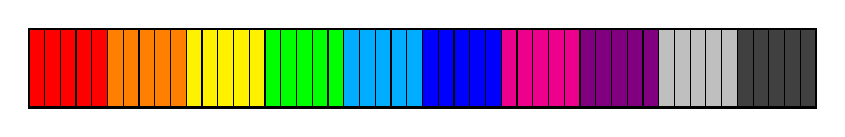
\begin{tikzpicture}
      \filldraw[fill=red]    (0, 0) rectangle  +(1,1);
      \filldraw[fill=orange] (1, 0) rectangle  +(1,1);
      \filldraw[fill=yellow] (2, 0) rectangle  +(1,1);
      \filldraw[fill=green]  (3, 0) rectangle  +(1,1);
      \filldraw[fill=cyan]   (4, 0) rectangle  +(1,1);
      \filldraw[fill=blue]   (5, 0) rectangle  +(1,1);
      \filldraw[fill=magenta] (6, 0) rectangle  +(1,1);
      \filldraw[fill=violet] (7, 0) rectangle +(1,1);
      \filldraw[fill=lightgray] (8, 0) rectangle +(1,1);
      \filldraw[fill=darkgray] (9, 0) rectangle +(1,1);
      
      \draw[thick] (0, 0) rectangle (10, 1);
      \foreach \i in {0.2, 0.4, ..., 9.8} {
        \draw (\i, 0) -- +(0, 1);
      }
    \end{tikzpicture}
  \end{center}
  
  \begin{enumerate}
  \item $P_i$ computes the sum $S_i$ of its own slice \hfill \alert{[local]}
  \item Distributed algorithm for $T \gets$ \mintinline{C}{exclusive_scan(0, p, S)}
    \begin{itemize}
    \item \texttt{MPI\_Exscan}
    \end{itemize}
  \item[$\rightarrow$] $P_i$ gets $T_i = $ sum of \emph{all previous} slices
  \item $P_i$ \mintinline{C}{exclusive_scan(T[i], ...)} its own slice \hfill \alert{[local]}
  \end{enumerate}

  \begin{alertblock}{Analysis}
    \vspace*{-2ex}
    \[
      T =  \text{[communication]} + \alert{2}\frac{n}{p} \text{ FLOP}
    \]
    \vspace*{-2ex}
  \end{alertblock}
\end{frame}

%%%%%%%%%%%%%%%%%%%%%%%%%%%%%%%%%%%%%%%%% 


\begin{frame}<1>[label=scan-algo]
  \frametitle{\texttt{MPI\_Exscan}}
  
  \begin{exampleblock}{Phase 1 : \texttt{reduce}}
    \begin{itemize}
    \item Input $x_i$
    \item Receive $u_0,  u_1, \dots$ from children
    \item Set $y_i \gets \sum u_j$. Send $x_i + y_i$ to father
    \end{itemize}
  \end{exampleblock}

  $\rightarrow \lceil \log_2 p \rceil$ successive messages of size 1

  \pause
  
  \begin{alertblock}{Phase 2 : \texttt{exclusive scan}}
    \begin{enumerate}
    \item Root: $w_i \gets 0$, otherwise receive $w_i$ from father
      \begin{itemize}
      \item[$=$] [sum of values of \emph{left} siblings]
      \end{itemize}
    \item Set $x_i \gets y_i + w_i$
    \item Sends $w_i + u_0 + \dots + u_{j-1}$ to the $j$-th children
      \begin{itemize}
      \item[$\leadsto$] Prefix-sum the $u_j$'s starting from $w_i$
      \end{itemize}
    \end{enumerate}
  \end{alertblock}

  $\rightarrow \lceil \log_2 p \rceil$ successive messages of size 1
\end{frame}

%%%%%%%%%%%%%%%%%%%%%%%%%%%%%%%%%%%%%%%%%%%%%%%%%%%%%%%%%%%%%%%%%%%%

\begin{frame}[label=scan]
  \frametitle{\texttt{MPI\_Reduce} Using the Binomial Tree Algorithm}
  
  \begin{center}
    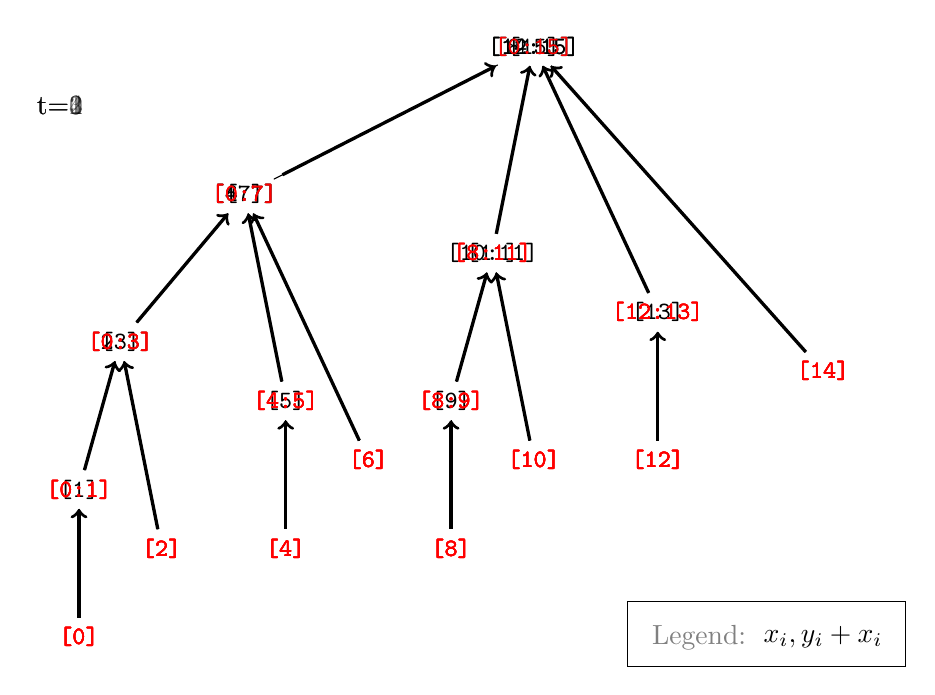
\begin{tikzpicture}[
        level distance=25mm, xscale=0.7, yscale=0.75,
        emph/.style={edge from parent/.style={draw, <-, very thick}},
        norm/.style={edge from parent/.style={draw, thin}}
      ]

      %%% 
      \path<1> [semitransparent,gray] (-8, -1) node[text=black,left] {t=0};
      \path<2> [semitransparent,gray] (-8, -1) node[text=black,left] {t=1};
      \path<3> [semitransparent,gray] (-8, -1) node[text=black,left] {t=2};
      \path<4> [semitransparent,gray] (-8, -1) node[text=black,left] {t=3};
      \path<5> [semitransparent,gray] (-8, -1) node[text=black,left] {t=4};

      \draw (1.7, -9.4) rectangle (6.75, -10.5);
      \node[gray] at (3, -10) {Legend:};
      \node at (5.25, -10) {$x_i, \alert{y_i + x_i}$};
      
      \begin{scope}[every node/.style={font=\small\ttfamily}]
          \node<1> {[15]}
    child { node {[7]}
      child { node {[3]}
        child {node {[1]}
          child[emph] {node[red] {[0]}}
        }
        child[emph] {node[red] at (0, -1) {[2]}}
      }
      child[missing]
      child {node at (0,-1) {[5]}
        child[emph] {node[red] {[4]}}
      }
      child[emph] {node[red] at (0,-2) {[6]} }
    }
    child[missing]
    child[missing]
    child { node at (0, -1) {[11]}
      child {node {[9]}
        child[emph] {node[red] {[8]} }
      }
      child[emph] {node[red] at (0, -1) {[10]} }
    }
    child[missing]
    child { node at (0, -2) {[13]}
      child[emph] {node[red] {[12]}}
    }
    child[missing]
    child[emph] { node[red] at (0, -3) {[14]} }
    ;
    
    %%%%%%

    \node<2> {[14:15]}
    child { node {[6:7]}
      child { node {[2:3]}
        child[emph] {node[red] {[0:1]}
          child[norm] {node[red] {[0]}}
        }
        child {node[red] at (0, -1) {[2]}}
      }
      child[missing]
      child[emph] {node[red] at (0,-1) {[4:5]}
        child[norm] {node[red] {[4]}}
      }
      child {node[red] at (0,-2) {[6]} }
    }
    child[missing]
    child[missing]
    child { node at (0, -1) {[10:11]}
      child[emph] {node[red] {[8:9]}
        child[norm] {node[red] {[8]} }
      }
      child {node[red] at (0, -1) {[10]} }
    }
    child[missing]
    child[emph] { node[red] at (0, -2) {[12:13]}
      child[norm] {node[red] {[12]}}
    }
    child[missing]
    child { node[red] at (0, -3) {[14]} }
    ;

    %%%%%% 

    \node<3> {[12:15]}
    child { node {[4:7]}
      child[emph] { node [red] {[0:3]}
        child[norm] {node[red] {[0:1]}
          child {node[red] {[0]}}
        }
        child[norm] {node[red] at (0, -1) {[2]}}
      }
      child[missing]
      child {node[red] at (0,-1) {[4:5]}
        child {node[red] {[4]}}
      }
      child {node[red] at (0,-2) {[6]} }
    }
    child[missing]
    child[missing]
    child[emph] { node[red] at (0, -1) {[8:11]}
      child[norm] {node[red] {[8:9]}
        child {node[red] {[8]} }
      }
      child[norm] {node[red] at (0, -1) {[10]} }
    }
    child[missing]
    child { node[red] at (0, -2) {[12:13]}
      child {node[red] {[12]}}
    }
    child[missing]
    child { node[red] at (0, -3) {[14]} }
    ;

    %%%%%% 

    \node<4> {[8:15]}
    child[emph] { node[red] {[0:7]}
      child[norm] { node [red] {[0:3]}
        child {node[red] {[0:1]}
          child {node[red] {[0]}}
        }
        child {node[red] at (0, -1) {[2]}}
      }
      child[missing]
      child[norm] {node[red] at (0,-1) {[4:5]}
        child {node[red] {[4]}}
      }
      child[norm] {node[red] at (0,-2) {[6]} }
    }
    child[missing]
    child[missing]
    child { node[red] at (0, -1) {[8:11]}
      child {node[red] {[8:9]}
        child {node[red] {[8]} }
      }
      child {node[red] at (0, -1) {[10]} }
    }
    child[missing]
    child { node[red] at (0, -2) {[12:13]}
      child {node[red] {[12]}}
    }
    child[missing]
    child { node[red] at (0, -3) {[14]} }
    ;

    \node<5>[red] {[0:15]}
    child { node[red] {[0:7]}
      child { node [red] {[0:3]}
        child {node[red] {[0:1]}
          child {node[red] {[0]}}
        }
        child {node[red] at (0, -1) {[2]}}
      }
      child[missing]
      child {node[red] at (0,-1) {[4:5]}
        child {node[red] {[4]}}
      }
      child {node[red] at (0,-2) {[6]} }
    }
    child[missing]
    child[missing]
    child { node[red] at (0, -1) {[8:11]}
      child {node[red] {[8:9]}
        child {node[red] {[8]} }
      }
      child {node[red] at (0, -1) {[10]} }
    }
    child[missing]
    child { node[red] at (0, -2) {[12:13]}
      child {node[red] {[12]}}
    }
    child[missing]
    child { node[red] at (0, -3) {[14]} }
    ;

  \end{scope}
\end{tikzpicture}
\end{center}
\end{frame}

%%%%%%%%%%%%%%%%%%%%%%%%%%%%%%%%%%%%%%%%%%%

\againframe<2>{scan-algo}

%%%%%%%%%%%%%%%%%%%%%%%%%%%%%%%%%%%

\begin{frame}[label=scan-tree]
  \frametitle{\texttt{MPI\_Exscan} Using the Binomial Tree Algorithm}

  \begin{center}
    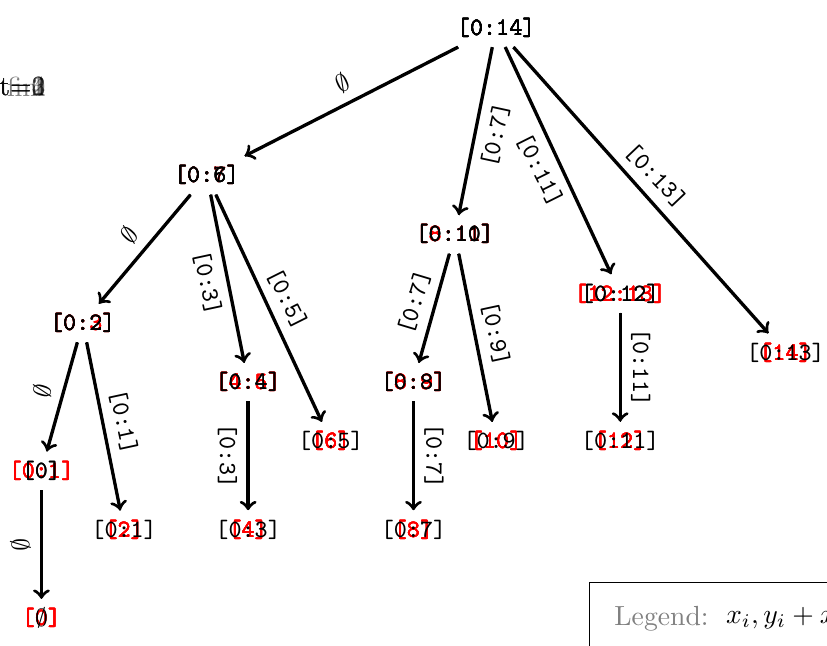
\begin{tikzpicture}[level distance=25mm, xscale=0.7, yscale=0.75,
      emph/.style={edge from parent/.style={draw, ->, very thick}},
      norm/.style={edge from parent/.style={draw, thin}},
      ]

      \path[use as bounding box] (-8.5, 0) rectangle (5.5, -10);
      
      %%%
    \path<1> [semitransparent,gray] (-8, -1) node[text=black,left] {t=0};
    \path<2> [semitransparent,gray] (-8, -1) node[text=black,left] {t=1};
    \path<3> [semitransparent,gray] (-8, -1) node[text=black,left] {t=2};
    \path<4> [semitransparent,gray] (-8, -1) node[text=black,left] {t=3};
    \path<5> [semitransparent,gray] (-8, -1) node[text=black,left] {t=4};
    \path<6> [semitransparent,gray] (-8, -1) node[text=black,left] {fini};

    \draw (1.7, -9.4) rectangle (6.75, -10.5);
    \node[gray] at (3, -10) {Legend:};
    \node at (5.25, -10) {$x_i, \alert{y_i + x_i}$};

    \begin{scope}[every node/.style={font=\small\ttfamily}]  

    \node<1> {[0:14]}          % initial state
    child { node[red] {[0:7]}
      child { node[red] {[0:3]}
        child {node[red] {[0:1]}
          child {node[red] {[0]}}
        }
        child {node[red] at (0, -1) {[2]}}
      }
      child[missing]
      child {node[red] at (0,-1) {[4:5]}
        child {node[red] {[4]}}
      }
      child {node[red] at (0,-2) {[6]} }
    }
    child[missing]
    child[missing]
    child { node[red] at (0, -1) {[8:11]}
      child {node[red] {[8:9]}
        child {node[red] {[8]} }
      }
      child {node[red] at (0, -1) {[10]} }
    }
    child[missing]
    child { node[red] at (0, -2) {[12:13]}
      child {node[red] {[12]}}
    }
    child[missing]
    child { node[red] at (0, -3) {[14]} }
    ;


    \node<2> {[0:14]}  % t==1
    child[emph] { node[red] {[0:7]}
      child[norm] { node[red]  {[0:3]}
        child {node[red]{[0:1]}
          child {node[red]{[0]}}
        }
        child {node[red]at (0, -1) {[2]}}
      }
      child[missing]
      child[norm] {node[red]at (0,-1) {[4:5]}
        child {node[red]{[4]}}
      }
      child[norm] {node[red]at (0,-2) {[6]} }
      edge from parent node[sloped, above] {$\emptyset$}
    }
    child[missing]
    child[missing]
    child { node[red]at (0, -1) {[8:11]}
      child {node[red]{[8:9]}
        child {node[red]{[8]} }
      }
      child {node[red]at (0, -1) {[10]} }
    }
    child[missing]
    child { node[red]at (0, -2) {[12:13]}
      child {node[red]{[12]}}
    }
    child[missing]
    child { node[red]at (0, -3) {[14]} }
    ;


    \node<3> {[0:14]}  % t==2
    child { node {[0:6]}
      child[emph] { node[red] {[0:3]}
        child[norm] {node[red]{[0:1]}
          child {node[red]{[0]}}
        }
        child[norm] {node[red]at (0, -1) {[2]}}
        edge from parent node[sloped,above] {$\emptyset$}
      }
      child[missing]
      child {node[red]at (0,-1) {[4:5]}
        child {node[red]{[4]}}
      }
      child[norm] {node[red]at (0,-2) {[6]} }
    }
    child[missing]
    child[missing]
    child[emph] { node[red]at (0, -1) {[8:11]}
      child[norm] {node[red]{[8:9]}
        child {node[red]{[8]} }
      }
      child[norm] {node[red]at (0, -1) {[10]} }
      edge from parent node[below,sloped] {[0:7]}      
    }
    child[missing]
    child { node[red]at (0, -2) {[12:13]}
      child {node[red]{[12]}}
    }
    child[missing]
    child { node[red]at (0, -3) {[14]} }
    ;


    \node<4> {[0:14]}   % t == 3
    child { node {[0:7]}
      child { node {[0:2]}
        child[emph] {node[red]{[0:1]}
          child[norm] {node[red]{[0]}}
          edge from parent node[above,sloped] {$\emptyset$}
        }
        child[norm] {node[red]at (0, -1) {[2]} }
      }
      child[missing]
      child[emph] { node[red]at (0,-1) {[4:5]}
        child[norm] {node[red]{[4]}}
        edge from parent node[below,sloped] {[0:3]} 
      }
      child {node[red]at (0,-2) {[6]}}
    }
    child[missing]
    child[missing]
    child[norm] { node at (0, -1) {[0:10]} 
      child[emph] {node[red]{[8:9]}
        child[norm] {node[red]{[8]} }
        edge from parent node[sloped,above] {[0:7]}
      }
      child[norm] {node[red]at (0, -1) {[10]} }
    }
    child[missing]
    child[emph] { node[red]at (0, -2) {[12:13]}
      child[norm] {node[red]{[12]}}
      edge from parent node[sloped,below] {[0:11]}
    }
    child[missing]
    child { node[red]at (0, -3) {[14]} }
    ;


    \node<5> {[0:14]}   % t == 4
    child { node {[0:6]}
      child { node {[0:2]}
        child {node {[0]}
          child[emph] {node[red] {[0]} edge from parent node[sloped,below] {$\emptyset$} }
        }
        child[emph] {node[red]at (0, -1) {[2]} edge from parent node[sloped,above] {[0:1]} }
      }
      child[missing]
      child {node at (0,-1) {[0:4]}
        child[emph] {node[red]{[4]} edge from parent node[sloped,below] {[0:3]}}
      }
      child[emph] {node[red]at (0,-2) {[6]} edge from parent node[sloped,above] {[0:5]}}
    }
    child[missing]
    child[missing]
    child { node at (0, -1) {[0:10]}
      child {node {[0:8]}
        child[emph] {node[red]{[8]} edge from parent node[sloped,above] {[0:7]} }
      }
      child[emph] {node[red]at (0, -1) {[10]} edge from parent node[sloped,above] {[0:9]} }
    }
    child[missing]
    child { node at (0, -2) {[0:12]}
      child[emph] {node[red]{[12]} edge from parent node[sloped,above] {[0:11]} }
    }
    child[missing]
    child[emph] { node[red]at (0, -3) {[14]} edge from parent node[sloped,above] {[0:13]} }
    ;

    \node<6> {[0:14]}  %final state
    child { node {[0:6]}
      child { node {[0:2]}
        child {node {[0]}
          child {node {$\emptyset$}}
        }
        child {node at (0, -1) {[0:1]}}
      }
      child[missing]
      child {node at (0,-1) {[0:4]}
        child {node {[0:3]}}
      }
      child {node at (0,-2) {[0:5]} }
    }
    child[missing]
    child[missing]
    child { node at (0, -1) {[0:11]}
      child {node {[0:8]}
        child {node {[0:7]} }
      }
      child {node at (0, -1) {[0:9]} }
    }
    child[missing]
    child { node at (0, -2) {[0:12]}
      child {node {[0:11]}}
    }
    child[missing]
    child { node at (0, -3) {[0:13]} }
    ;

  \end{scope}
\end{tikzpicture}
\end{center}
\end{frame}


\section{Linear Algebra}

%%%%%%%%%%%%%%%%%%%%%%%%%%%%%%%%%%%%%%%%%%%%%%%%%%%%%%

\begin{frame}
  \centering
  \vfill
  \Huge Linear Algebra
  \vfill
\end{frame}

\begin{frame}
  \frametitle{Importance of Linear Algebra}

  \begin{alertblock}{Reason}
  Systems of \textbf{linear} equations are the only ones we can solve
    \begin{itemize}
    \item (efficiently, at least)
    \end{itemize}
  \end{alertblock}

  \begin{itemize}
  \item $Ax = b$
  \item $AX = B$  \hfill (multiple right-hand sides)
  \item $\min_x \| Ax - b \|_2$ \hfill (overdetermined linear least squares)
  \item $\min_x \| x \|_2$ s.t. $Ax = b$ \hfill (underdetermined linear least squares)
  \item $Av = \lambda v$ \hfill (eigenvalues/eigenvectors)

  \end{itemize}

  \medskip

  \begin{center}
    \fbox{Basic building block of nearly all scientific computation}
  \end{center}
\end{frame}

%%%%%%%%%%%%%%%%%%%%%%%%%%%%%%%%%%%%%%%%%%%%%%%%%%%%%%

\subsection{Dense}
\subsubsection{BLAS interface and data representation}

\begin{frame}[label=blas]
  \frametitle{BLAS}

  % how to write fast software?
  % use the right tools
  % small set of vesratile and optimized libraries
  
  \begin{block}{Basic Linear Algebra Subroutines}
    \begin{itemize}
    \item Software libraries developed in the 1980's (Fortran-77...)
    \item \red{Simple} and \red{common} operations
    \item \red{heavily optimized}
      \begin{itemize}
      \item[$\Rightarrow$] you will never do better
      \end{itemize}
    \end{itemize}
  \end{block}

  \begin{exampleblock}{Common HPC Design Strategy}
    \begin{itemize}
    \item More complex linear algebra use the BLAS
    \item Simplifies development
      \begin{itemize}
      \item Just need to remember the interface
      \end{itemize}
    \item High-speed BLAS $\leadsto$ high-speed software
    \item Ugly low-level optimizations \emph{confined} inside the BLAS
    \end{itemize}
  \end{exampleblock}  
\end{frame}

%%%%%%%%%%%%%%%%%%%%%%%%%%%%%%%%%%%%%%%%%%%%%%%%%%%%%%

\begin{frame}[label=blas]
  \frametitle{BLAS Levels}

  \[
    \texttt{x} \in \{ \texttt{S}, \texttt{D}, \texttt{C}, \texttt{Z} \}
  \]
  
  \begin{block}{Level 1 Routines: \red{vector} operations}
    \begin{itemize}
    \item \texttt{xSCAL} : $x \gets \alpha x$
    \item \texttt{xCOPY} : $x \gets y$
    \item \texttt{xAXPY} : $y \gets \alpha x + y$
    \item \texttt{xDOT} : $\alpha \gets x \cdot y$
    \item \texttt{xNORM} : $\alpha \gets \| x \|_2$
    \item \texttt{xSUM} : $k \gets \sum_i | x_i |$
    \item \texttt{IxAMAX} : $k \gets \argmax_i | x_i |$
    \end{itemize}
  \end{block}
\end{frame}

%%%%%%%%%%%%%%%%%%%%%%%%%%%%%%%%%%%%%%%%%%%%%%%%%%%%%%%%%%%%%%

\begin{frame}[label=blas]
  \frametitle{BLAS Levels}

  \[
    \texttt{x} \in \{ \texttt{S}, \texttt{D}, \texttt{C}, \texttt{Z} \}
  \]
  
  \begin{block}{Level 2 Routines: \red{matrix-vector} operations}
    \begin{itemize}
    \item Matrix-vector product (\texttt{xGEMV}) 
      \begin{itemize}
      \item $y \gets \alpha Ax + \beta y$
      \item Options to multiply by $A^t$ or $A^h$
      \item Special cases: symmetric $A$ (\texttt{xSYMV}), triangular $A$ (\texttt{xTRMV})
      \end{itemize}

      \medskip
      
    \item Triangular solve (\texttt{xTRSV})
      \begin{itemize}
      \item Solve $Lx = b$ or $Ux = b$
      \end{itemize}

      \medskip
      
    \item Rank-1 update (\texttt{xGER})
      \begin{itemize}
      \item $A \gets A + \alpha x y^t$        
      \end{itemize}
    \end{itemize}
  \end{block}
\end{frame}

%%%%%%%%%%%%%%%%%%%%%%%%%%%%%%%%%%%%%%%%%%%%%%%%%%%%%%%%%%%%%%

\begin{frame}[label=blas]
  \frametitle{BLAS Levels}

  \[
    \texttt{x} \in \{ \texttt{S}, \texttt{D}, \texttt{C}, \texttt{Z} \}
  \]
  
  \begin{block}{Level 3 Routines: \red{matrix-matrix} operations}
    \begin{itemize}
    \item Matrix-Matrix product (\texttt{xGEMM}) 
      \begin{itemize}
      \item $C \gets \alpha AB + \beta C$
      \item Options to use $A^t$ or $B^t$
      \item Special cases: symmetric $A,B$ (\texttt{xSYMM}), triangular $A$ (\texttt{xTRMM})
      \end{itemize}

      \medskip
      
    \item Triangular solve (\texttt{xTRSM}) with multiple right-hand sides
      \begin{itemize}
      \item Solve $LX = B$ or $UX = B$
      \end{itemize}

      \medskip
      
    \item Rank-$k$ symmetric update (\texttt{xSYRK})
      \begin{itemize}
      \item $C \gets \alpha AA^t + \beta C$ 
      \item Symmetric $C$ (otherwise it is just \texttt{xGEMM})
      \end{itemize}
    \end{itemize}
  \end{block}
\end{frame}

%%%%%%%%%%%%%%%%%%%%%%%%%%%%%%%%%%%%%%%%%%%%%%%%%%%%%%%%%%%%%%%%%%%%%%%%%%%%%%%%%%%%%%%%%

\begin{frame}[label=blasdata,fragile=singleslide]
  \frametitle{Data Representation}

  \begin{exampleblock}{Matrices represented as \textbf{\alert{1D arrays}}}
    \vspace*{-2ex}
    \[
      \begin{pmatrix}
        0 & 1 & 2 & 3 \\
        4 & 5 & 6 & 7 \\
        8 & 9 & a & b
      \end{pmatrix}
    \]
    \vspace*{-2ex}
    \begin{itemize}
    \item Memory: \mintinline{C}{[0, 1, 2, 3, 4, 5, 6, 7, 8, 9, 0xa, 0xb]}
    \item \textbf{Never ever} as array of pointers to arrays
    \end{itemize}
  \end{exampleblock}
  
  \begin{alertblock}{\mintinline{C}{double **A} is \textbf{banished}}
    \begin{itemize}
    \item Can write \mintinline{C}{A[i][j]} \smiley
    \item Accessing \mintinline{C}{A[i + 1][j]} is \textbf{costly} \triste (indirection)
    \item Pointers take space \triste
    \item \mintinline{C}{malloc()} takes time (how much?) \triste
    \item Allocation complex and error-prone \triste
    \end{itemize}
  \end{alertblock}
\end{frame}

%%%%%%%%%%%%%%%%%%%%%%%%%%%%%%%%%%%%%%%%%%%%%%%%%%%%%%%%%%%%%%%%%%%%%%%%%%%%%%%%%%%%%%%%

\begin{frame}[label=blasdata]
  \frametitle{Data Representation (continued)}

  \begin{block}{Flat arrays: two possible orderings}
    \begin{itemize}
    \item Memory: \mintinline{C}{[0, 1, 2, 3, 4, 5, 6, 7, 8, 9, 0xa, 0xb]}
    \item Row-major order (C, Pascal)
      \[
        \begin{pmatrix}
          0 & 1 & 2 & 3 \\
          4 & 5 & 6 & 7 \\
          8 & 9 & a & b
        \end{pmatrix}
      \]
      
    \item Column-major order (Fortran, matlab, julia, R)
      \[
        \begin{pmatrix}
          0 & 3 & 6 & 9 \\
          1 & 4 & 7 & a \\
          2 & 5 & 8 & b
        \end{pmatrix}
      \]
    \end{itemize}
  \end{block}
\end{frame}


%%%%%%%%%%%%%%%%%%%%%%%%%%%%%%%%%%%%%%%%%%%%%%%%%%%%%%%%%%%%%%%%%%%%%%%%%%%%%%%%%%%%%%%%

\begin{frame}[label=blasdata,fragile]
  \frametitle{Data Representation (continued)}

  \begin{exampleblock}{Matrix given by}
    \begin{itemize}
    \item Memory address of first coefficient
    \item \#Rows ($m$)
    \item \#Columns ($n$)
    \item Leading dimension (``stride'')
      \begin{itemize}
      \item Sub-matrices for free
      \end{itemize}
    \end{itemize}
  \end{exampleblock}

  \begin{columns}
    \begin{column}{5.33cm}
      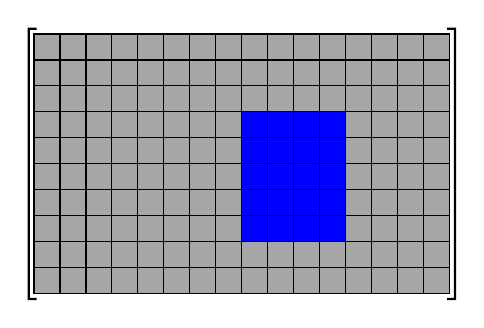
\begin{tikzpicture}[scale=0.66]
%        \draw[red,dotted,use as bounding box] (0, 0) rectangle (5, 5);
        \tikzmat{0,0}{8,5}
        \filldraw[fill=Gray!70] (0, 0) rectangle (8,5);
        \filldraw<2->[fill=blue] (4, 1) rectangle +(2,2.5);
        \foreach \i in {0.5, 1, ..., 4.5} {
          \draw (0, \i) -- +(8, 0);
        }
        \foreach \i in {0.5, 1, ..., 7.5} {
          \draw (\i, 0) -- +(0, 5);
        }
      \end{tikzpicture}
    \end{column}
    \begin{column}{6.66cm}
      \begin{itemize}
      \item Row-major (\mintinline{C}{ld >= n})
        \begin{itemize}
        \item $M_{ij} \leadsto \texttt{A[i*ld + j]}$
        \item {\color{Gray} $A, m = 10$, $n = 16$, $ld = 16$}
        \item<2-> {\color{blue} $A + 57, m = 5$, $n = 4$, $ld = 16$}
        \end{itemize}
      \item Column-major (\mintinline{C}{ld >= m})      
        \begin{itemize}
        \item $M_{ij} \leadsto \texttt{A[j*ld + i]}$
        \item {\color{Gray} $A, m = 10$, $n = 16$, $ld = 10$}
        \item<2-> {\color{blue} $A + 84, m = 5$, $n = 4$, $ld = 10$}
        \end{itemize}
      \end{itemize}  
    \end{column}
  \end{columns}
\end{frame}

%%%%%%%%%%%%%%%%%%%%%%%%%%%%%%%%%%%%%%%%%%%%%%%%%%%%%%%%%%%%%%%%%%%%%%%%%%%%%%%%%%%%%%%%

\begin{frame}[label=blasdata]
  \frametitle{Data Representation (continued)}

  \begin{exampleblock}{Vector given by}
    \begin{itemize}
    \item Memory address of first coefficient
    \item Size ($n$)
    \item Increment (``stride'')
    \end{itemize}
  \end{exampleblock}

  \begin{columns}
    \begin{column}{5.33cm}
      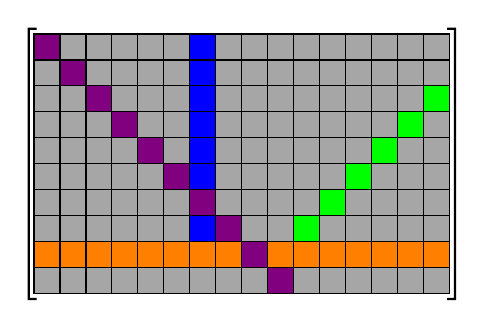
\begin{tikzpicture}[scale=0.66]
        \tikzmat{0,0}{8,5}
        \filldraw[fill=Gray!70] (0, 0) rectangle (8,5);
        \filldraw<2->[fill=orange] (0, 0.5) rectangle +(8,0.5);
        \filldraw<3->[fill=blue] (3, 1) rectangle +(0.5, 4);
        \foreach \i in {0, 0.5, ..., 4.5} {
          \filldraw<4->[fill=violet] (\i, 4.5-\i) rectangle +(0.5, 0.5);
        }
        \foreach \i in {1, 1.5, ..., 3.5} {
          \filldraw<5->[fill=green] (\i + 4, \i) rectangle +(0.5, 0.5);
        }
        \foreach \i in {0.5, 1, ..., 4.5} {
          \draw (0, \i) -- +(8, 0);
        }
        \foreach \i in {0.5, 1, ..., 7.5} {
          \draw (\i, 0) -- +(0, 5);
        }
      \end{tikzpicture}

    \end{column}
    \begin{column}{6.66cm}

      \begin{itemize}
      \item Row-major ($M_{ij} \leadsto \texttt{A[i*ld + j]}$)
        \begin{itemize}
        \item<2-> {\color{orange} $A + 128, n=16$, $i = 1$}
        \item<3-> {\color{blue} $A + 6, n = 8$, $i = 16$}
        \item<4-> {\color{violet} $A, n = 10$, $i = 17$}
        \item<5-> $A + 31, n = 6$, $i = 15$

        \end{itemize}
      \end{itemize}  
    \end{column}
  \end{columns}
\end{frame}

%%%%%%%%%%%%%%%%%%%%%%%%%%%%%%%%%%%%%%%%%%%%%%%%%%%%%%%%%%%%%%%%%%%%

\subsubsection{xGER}

\begin{frame}[label=ger,fragile]
  \frametitle{Rank-1 update (\mintinline{C}{xGER})}
  \framesubtitle{$A \gets A + \alpha x y^t$}

  \begin{center}
    \begin{tikzpicture}[scale=0.75]
      \begin{scope}
        \tikzmat{0,0}{5, 7}
        \filldraw[fill=red] (0, 0) rectangle node {$A$} +(5, 7);
      \end{scope}
      \node at (5.7, 3.5) {+=};
      \begin{onlyenv}<1>
      \begin{scope}[xshift=6.4cm]
        \tikzmat{0,0}{0.5, 7}
        \filldraw[fill=cyan] (0, 0) rectangle node[font=\small] {$x$} +(0.5, 7);
      \end{scope}
      \begin{scope}[xshift=7.2cm, yshift=6.5cm]
        \tikzmat{0,0}{5,0.5}
        \filldraw[fill=green] (0, 0) rectangle node[font=\small] {$y^t$} +(5, 0.5);
      \end{scope}
      \end{onlyenv}
      \begin{onlyenv}<2->
        \tikzmat{6.4,0}{11.4,7}
        \shade[left color=green, right color=cyan, shading angle=45] (6.4, 0) rectangle +(5, 7);
        \path<2> (6.4, 0) rectangle node[font=\small] {$xy^t$} +(5, 7);
        \path<3> (6.4, 0) rectangle node[font=\small] {$x_iy_j$} +(5, 7);
      \end{onlyenv}
    \end{tikzpicture}
  \end{center}
\end{frame}


\begin{frame}[label=ger,fragile]
  \frametitle{Double-Precision Rank-1 update (\mintinline{C}{DGER})}
  \framesubtitle{$A \gets A + \alpha x y^t$}

  \vspace*{-2ex}
  
  \begin{overlayarea}{12cm}{6.5cm}
    \begin{onlyenv}<1>
      \begin{wider}
  \begin{minted}[fontsize=\footnotesize]{C}
void dGER(int m, int n, double alpha, double *x, int incx,
          double *y, int incy, double *A, int ldA)
{
    for (int i = 0; i < m; i++)
        for (int j = 0; j < n; j++)
            A[i * ldA + j] += alpha * x[i * incx] * y[j * incy];
}
  \end{minted}
\end{wider}
\end{onlyenv}

\begin{onlyenv}<2>
  \begin{wider}
    \begin{minted}[fontsize=\footnotesize]{C}
void dGER(int m, int n, double alpha, double *x, int incx,
          double *y, int incy, double *A, int ldA)
{
    int ix = 0, iA = 0;
    for (int i = 0; i < m; i++) {
        double tmp = alpha * x[ix];
        int jy = 0;
        for (int j = 0; j < n; j++) {
            A[iA + j] += tmp * y[jy];
            jy += incy;
        }
        ix += incx;
        iA += ldA;    
    }
}
        \end{minted}
      \end{wider}
    \end{onlyenv}
  \end{overlayarea}
%%%% 

  \begin{onlyenv}<1>
    \begin{itemize}
    \item $3mn$ integer multiplications, $2mn + m$ integer additions
    \item $3mn$ FLOP
    \item $4mn$ memory accesses
    \end{itemize}
  \end{onlyenv}

  \begin{onlyenv}<2>
    \begin{itemize}
    \item \alert{0} integer multiplications, $2mn + 2m$ integer additions
    \item $\alert{2}nm + m$ FLOP
    \item $\alert{3}mn + m$ memory accesses
    \end{itemize}
  \end{onlyenv}
\end{frame}

%%%%%%%%%%%%%%%%%%%%%%%%%%%%%%%%%%%%%%%%%%%%%%%%%%%%%%%%%%%%%%%%%%%%

\begin{frame}[label=block-cyclic,fragile=singleslide]
\frametitle{1D Block-Cyclic Distribution}

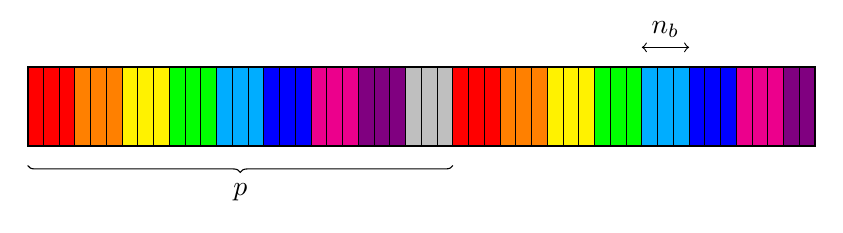
\begin{tikzpicture}
  \path[use as bounding box] (0, -0.75) rectangle (10, 1.5);
  \draw[thick] (0, 0) rectangle (10, 1);

  
  \draw[<->] (7.8, 1.25) -- node[above] {$n_b$} +(0.6, 0);
%  \draw[<->] (0, 2) -- node[above] {$n$} +(10, 0);
  \draw[decorate,decoration={brace,mirror}] (0, -0.25) -- node[below=1mm] {$p$} +(9*0.6, 0);

  \clip (0, 0) rectangle (10, 1);
  \foreach \i in {0, 5.4, 10.8} {
    \filldraw[fill=red]       (\i,       0) rectangle  +(0.6,1);
    \filldraw[fill=orange]    (\i + 0.6, 0) rectangle  +(0.6,1);
    \filldraw[fill=yellow]    (\i + 1.2, 0) rectangle  +(0.6,1);
    \filldraw[fill=green]     (\i + 1.8, 0) rectangle  +(0.6,1);
    \filldraw[fill=cyan]      (\i + 2.4, 0) rectangle  +(0.6,1);
    \filldraw[fill=blue]      (\i + 3.0, 0) rectangle  +(0.6,1);
    \filldraw[fill=magenta]   (\i + 3.6, 0) rectangle  +(0.6,1);
    \filldraw[fill=violet]    (\i + 4.2, 0) rectangle  +(0.6,1);
    \filldraw[fill=lightgray] (\i + 4.8, 0) rectangle  +(0.6,1);
    \filldraw[fill=darkgray]  (\i + 5.4, 0) rectangle  +(0.6,1);
  }
  \draw[thick] (0, 0) rectangle (10, 1);
  \foreach \i in {0.2, 0.4, ..., 9.8}
  \draw (\i, 0) -- +(0, 1);
\end{tikzpicture}

\begin{itemize}
\item 3 parameters: $(n, n_b, p)$
\item Element $i$ belongs to process $\lfloor i / n_b \rfloor \bmod p$
\end{itemize}

\vspace{-2ex}

\begin{wider}
\begin{minted}[fontsize=\footnotesize]{C}
/* returns the number of items I have */
int my_size(int n, int nb, int p, int rank)
{
    int nblocks = n / nb;                          /* #full blocks */
    int res = (nblocks / p) * nb;                    /* lower-bound */
    int extrablocks = nblocks % p;
    if (rank < extrablocks)               /* I have an extra block */
        res += nb;
    if (rank == extrablocks)              /* I have the last block */
          res += n % nb;
    return res;
}
\end{minted}
\end{wider}
\end{frame}

%%%%%%%%%%%%%%%%%%%%%%%%%%%%%%%%%%%%%%%%%%%%%%%%%%%%%%%%%%%%%%%%%%%%%%%%

\begin{frame}[label=block-cyclic]
\frametitle{2D Block-Cyclic Distribution}

\begin{columns}
  \begin{column}{6cm}

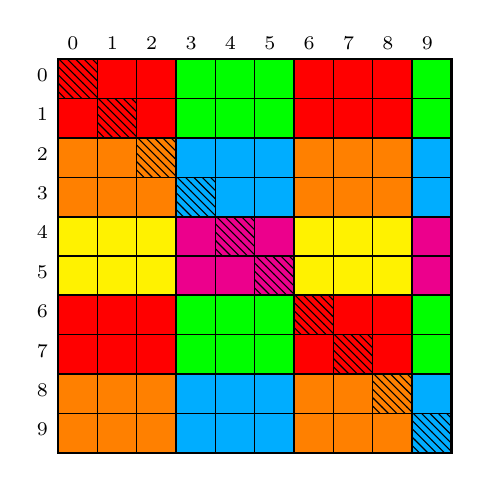
\begin{tikzpicture}[scale=0.5]
  \filldraw[fill=red]    (0, 8) rectangle  +(3, 2);
  \filldraw[fill=green]  (3, 8) rectangle  +(3, 2);
  \filldraw[fill=red]    (6, 8) rectangle  +(3, 2);
  \filldraw[fill=green]  (9, 8) rectangle  +(1, 2);

  \filldraw[fill=orange] (0, 6) rectangle  +(3, 2);
  \filldraw[fill=cyan]   (3, 6) rectangle  +(3, 2);
  \filldraw[fill=orange] (6, 6) rectangle  +(3, 2);
  \filldraw[fill=cyan]   (9, 6) rectangle  +(1, 2);

  \filldraw[fill=yellow]  (0, 4) rectangle  +(3, 2);
  \filldraw[fill=magenta] (3, 4) rectangle  +(3, 2);
  \filldraw[fill=yellow]  (6, 4) rectangle  +(3, 2);
  \filldraw[fill=magenta] (9, 4) rectangle  +(1, 2);
  
  \filldraw[fill=red]    (0, 2) rectangle  +(3, 2);
  \filldraw[fill=green]  (3, 2) rectangle  +(3, 2);
  \filldraw[fill=red]    (6, 2) rectangle  +(3, 2);
  \filldraw[fill=green]  (9, 2) rectangle  +(1, 2);
  
  \filldraw[fill=orange] (0, 0) rectangle  +(3, 2);
  \filldraw[fill=cyan]   (3, 0) rectangle  +(3, 2);
  \filldraw[fill=orange] (6, 0) rectangle  +(3, 2);
  \filldraw[fill=cyan]   (9, 0) rectangle  +(1, 2);

  \foreach \i in {0, ..., 9} {
    \fill[pattern=north west lines] (\i, 9-\i) rectangle +(1, 1);
  }
  \draw[thick] (0, 0) rectangle (10, 10);
  \foreach \i in {1, 2, ..., 9} {
    \draw (\i, 0) -- +(0, 10);
    \draw (0, \i) -- +(10, 0);
  }

  \foreach \i in {2, 4, ..., 8} {
    \draw[thick] (0, \i) -- +(10, 0);
  }
  \foreach \i in {3, 6, 9} {
    \draw[thick] (\i, 0) -- +(0, 10);
  }

  \foreach \i in {0, 1, ..., 9} {
    \node[anchor=south west,font=\scriptsize] at (\i, 10) {\i};
    \node[anchor=north east,font=\scriptsize] at (0, 10-\i) {\i};
  }


\end{tikzpicture}
\end{column}

\begin{column}{6cm}
  \begin{itemize}
  \item Matrix: $m \times n$ 
  \item Process grid: $P \times Q$
  \item Block size: $v \times h$
  \end{itemize}

  \begin{exampleblock}{Special cases}
    \begin{itemize}
    \item By block
      \begin{itemize}
      \item $v = m / P$
      \item $h = n / Q$
      \end{itemize}
    
    
    \item Purely Cyclic
      \begin{itemize}
      \item $v = 1$
      \item $h = 1$
      \end{itemize}

    \item 1D
      \begin{itemize}
      \item $h = n$ or $v = m$
      \end{itemize}
    \end{itemize}

  \end{exampleblock}
  
\end{column}
\end{columns}
\end{frame}

%%%%%%%%%%%%%%%%%%%%%%%

\begin{frame}[label=block-cyclic, fragile]
  \frametitle{2D Block-Cyclic Distribution}

  \begin{columns}
    \begin{column}{5.5cm}
  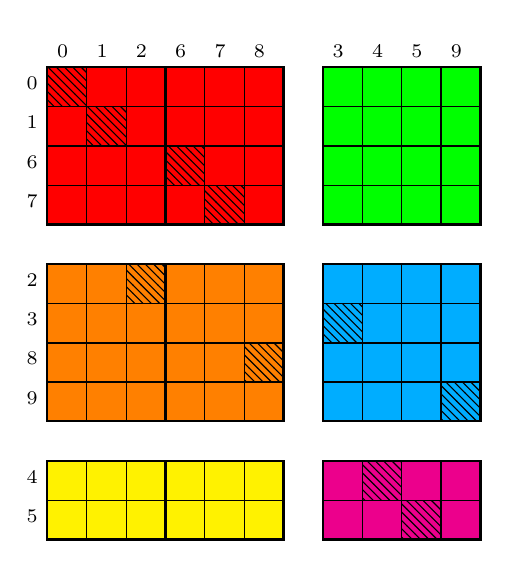
\begin{tikzpicture}[scale=0.5]
    \path[use as bounding box] (-0.5, 2) rectangle (11, 15);

    \filldraw[fill=red]     (0, 10) rectangle +(6, 4);
    \filldraw[fill=green]   (7, 10) rectangle +(4, 4);
    \filldraw[fill=orange]  (0, 5) rectangle  +(6, 4);
    \filldraw[fill=cyan]    (7, 5) rectangle  +(4, 4);
    \filldraw[fill=yellow]  (0, 2) rectangle  +(6, 2);
    \filldraw[fill=magenta] (7, 2) rectangle  +(4, 2);

    \fill[pattern=north west lines] (0, 13) rectangle +(1, 1);
    \fill[pattern=north west lines] (1, 12) rectangle +(1, 1);
    \fill[pattern=north west lines] (2, 8) rectangle +(1, 1);
    \fill[pattern=north west lines] (7, 7) rectangle +(1, 1);
    \fill[pattern=north west lines] (8, 3) rectangle +(1, 1);
    \fill[pattern=north west lines] (9, 2) rectangle +(1, 1);
    \fill[pattern=north west lines] (3, 11) rectangle +(1, 1);
    \fill[pattern=north west lines] (4, 10) rectangle +(1, 1);
    \fill[pattern=north west lines] (5,  6) rectangle +(1, 1);
    \fill[pattern=north west lines] (10,  5) rectangle +(1, 1);

      \foreach \q in {1, 2} {
        \begin{scope}[xshift = 0, yshift=\q*5cm]
          \draw[thick] (0, 0) rectangle (6, 4);
          \foreach \i in {1, 2, ..., 5} {
            \draw (\i, 0) -- +(0, 4);
          }
          \foreach \i in {1, 2, 3} {
            \draw (0, \i) -- +(6, 0);
          }
          \draw[thick] (0, 2) -- +(6, 0);
          \draw[thick] (0, 4) -- +(6, 0);
          \draw[thick] (3, 0) -- +(0, 4);
        \end{scope}
      }

      \begin{scope}[xshift = 0, yshift=2cm]
        \draw[thick] (0, 0) rectangle (6, 2);
        \foreach \i in {1, 2, ..., 5} {
          \draw (\i, 0) -- +(0, 2);
        }
        \draw (0, 1) -- +(6, 0);
        \draw[thick] (3, 0) -- +(0, 2);
      \end{scope}
      
      
      \foreach \q in {1, 2} {
        \begin{scope}[xshift = 7cm, yshift=\q*5cm]
          \draw[thick] (0, 0) rectangle (4, 4);
          \foreach \i in {1, 2, 3} {
            \draw (\i, 0) -- +(0, 4);
          }
          \foreach \i in {1, 2, 3} {
            \draw (0, \i) -- +(4, 0);
          }
          \draw[thick] (0, 2) -- +(4, 0);
          \draw[thick] (0, 4) -- +(4, 0);
          \draw[thick] (3, 0) -- +(0, 4);

        \end{scope}
      }
      \begin{scope}[xshift = 7cm, yshift=2cm]
        \draw[thick] (0, 0) rectangle (4, 2);
        \foreach \i in {1, 2, 3} {
          \draw (\i, 0) -- +(0, 2);
        }
        \draw (0, 1) -- +(4, 0);
        \draw[thick] (3, 0) -- +(0, 2);
      \end{scope}


    \node[anchor=south west,font=\scriptsize] at (0, 14) {0};
    \node[anchor=south west,font=\scriptsize] at (1, 14) {1};
    \node[anchor=south west,font=\scriptsize] at (2, 14) {2};
    \node[anchor=south west,font=\scriptsize] at (3, 14) {6};
    \node[anchor=south west,font=\scriptsize] at (4, 14) {7};
    \node[anchor=south west,font=\scriptsize] at (5, 14) {8};

    \node[anchor=south west,font=\scriptsize] at (7, 14)  {3};
    \node[anchor=south west,font=\scriptsize] at (8, 14)  {4};
    \node[anchor=south west,font=\scriptsize] at (9, 14)  {5};
    \node[anchor=south west,font=\scriptsize] at (10, 14) {9};
    
    \node[anchor=north east,font=\scriptsize] at (0, 14) {0};
    \node[anchor=north east,font=\scriptsize] at (0, 13) {1};
    \node[anchor=north east,font=\scriptsize] at (0, 12) {6};
    \node[anchor=north east,font=\scriptsize] at (0, 11) {7};

    \node[anchor=north east,font=\scriptsize] at (0, 9) {2};
    \node[anchor=north east,font=\scriptsize] at (0, 8) {3};
    \node[anchor=north east,font=\scriptsize] at (0, 7) {8};
    \node[anchor=north east,font=\scriptsize] at (0, 6) {9};

    \node[anchor=north east,font=\scriptsize] at (0, 4) {4};
    \node[anchor=north east,font=\scriptsize] at (0, 3) {5};
  \end{tikzpicture}
\end{column}

\begin{column}{6.5cm}
  \begin{itemize}
  \item Rows distributed block-cyclically 
  \item Cols distributed block-cyclically 
  \item[$\leadsto$] \alert{6} parameters
    \begin{itemize}
    \item $(m, n, v, h, P, Q)$
    \end{itemize}
    \medskip

  \item Each process has a ``local'' matrix
    \begin{itemize}
    \item Its blocks stacked together
    \item With a stride!
    \end{itemize}
  \item Not the same size everywhere!
    \begin{itemize}
    \item {\footnotesize \mintinline{C}{my_size(m, v, p, rank)}} rows
    \item {\footnotesize\mintinline{C}{my_size(n, h, q, rank)}} cols
    \end{itemize}
  \end{itemize}
\end{column}
\end{columns}

  \begin{alertblock}{Exercise for next week}
    Write a function that compute the \textbf{trace} (sum of diagonal elements)
    of a block-cyclically distributed matrix.
  \end{alertblock}

\end{frame}


%%%%%%%%%%%%%%%%%%%%%%%%%%%%%%%%%%%%%%%%%%%%%%%%%%%%%%%%%%%%%%%%%%

\begin{frame}[label=block-cyclic, fragile]
  \frametitle{\mintinline{C}{xGER} in Block-Cyclic Distribution}

  \begin{columns}
    \begin{column}{7cm}
  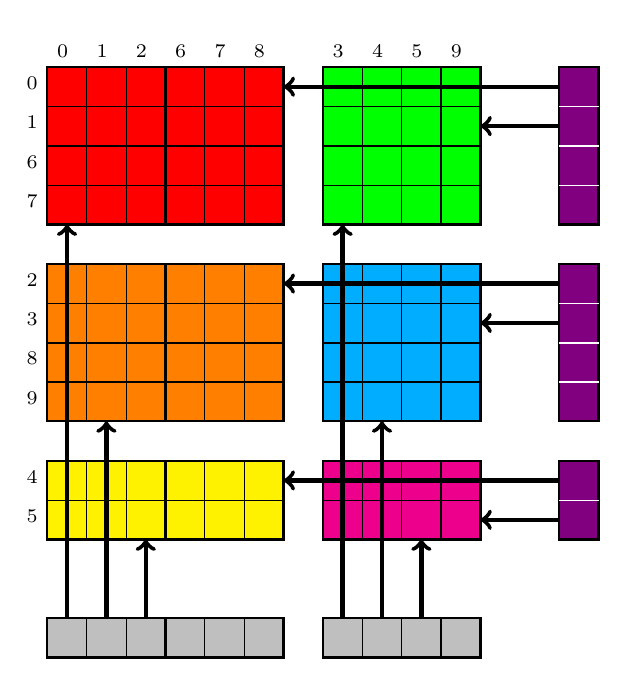
\begin{tikzpicture}[scale=0.5]
    \path[use as bounding box] (-0.5, -1) rectangle (14, 15);
    \filldraw<2->[thick, fill=lightgray]     (0, -1) rectangle +(6, 1);
    \filldraw<2->[thick, fill=lightgray]     (7, -1) rectangle +(4, 1);
    \filldraw<2->[thick, fill=violet]     (13, 2) rectangle +(1, 2);
    \filldraw<2->[thick, fill=violet]     (13, 5) rectangle +(1, 4);
    \filldraw<2->[thick, fill=violet]     (13, 10) rectangle +(1, 4);

    
    
    \foreach \i in {3, 6, 7, 8, 11, 12, 13} {
      \draw<2->[white] (13, \i) -- +(1, 0);
    }
    \draw<2->[white,thick] (13, 7) -- +(1, 0);
    \draw<2->[white,thick] (13, 12) -- +(1, 0);
    \foreach \i in {1, 2, 3, 4, 5, 8, 9, 10} {
      \draw<2-> (\i, -1) -- +(0, 1);
    }
    \draw<2->[thick] ( 3, -1) -- +(0, 1);
    \draw<2->[thick] (10, -1) -- +(0, 1);

    \filldraw[fill=red]     (0, 10) rectangle +(6, 4);
    \filldraw[fill=green]   (7, 10) rectangle +(4, 4);
    \filldraw[fill=orange]  (0, 5) rectangle  +(6, 4);
    \filldraw[fill=cyan]    (7, 5) rectangle  +(4, 4);
    \filldraw[fill=yellow]  (0, 2) rectangle  +(6, 2);
    \filldraw[fill=magenta] (7, 2) rectangle  +(4, 2);

      \foreach \q in {1, 2} {
        \begin{scope}[xshift = 0, yshift=\q*5cm]
          \draw[thick] (0, 0) rectangle (6, 4);
          \foreach \i in {1, 2, ..., 5} {
            \draw (\i, 0) -- +(0, 4);
          }
          \foreach \i in {1, 2, 3} {
            \draw (0, \i) -- +(6, 0);
          }
          \draw[thick] (0, 2) -- +(6, 0);
          \draw[thick] (0, 4) -- +(6, 0);
          \draw[thick] (3, 0) -- +(0, 4);
        \end{scope}
      }

      \begin{scope}[xshift = 0, yshift=2cm]
        \draw[thick] (0, 0) rectangle (6, 2);
        \foreach \i in {1, 2, ..., 5} {
          \draw (\i, 0) -- +(0, 2);
        }
        \draw (0, 1) -- +(6, 0);
        \draw[thick] (3, 0) -- +(0, 2);
      \end{scope}
      
      
      \foreach \q in {1, 2} {
        \begin{scope}[xshift = 7cm, yshift=\q*5cm]
          \draw[thick] (0, 0) rectangle (4, 4);
          \foreach \i in {1, 2, 3} {
            \draw (\i, 0) -- +(0, 4);
          }
          \foreach \i in {1, 2, 3} {
            \draw (0, \i) -- +(4, 0);
          }
          \draw[thick] (0, 2) -- +(4, 0);
          \draw[thick] (0, 4) -- +(4, 0);
          \draw[thick] (3, 0) -- +(0, 4);

        \end{scope}
      }
      \begin{scope}[xshift = 7cm, yshift=2cm]
        \draw[thick] (0, 0) rectangle (4, 2);
        \foreach \i in {1, 2, 3} {
          \draw (\i, 0) -- +(0, 2);
        }
        \draw (0, 1) -- +(4, 0);
        \draw[thick] (3, 0) -- +(0, 2);
      \end{scope}


    \node[anchor=south west,font=\scriptsize] at (0, 14) {0};
    \node[anchor=south west,font=\scriptsize] at (1, 14) {1};
    \node[anchor=south west,font=\scriptsize] at (2, 14) {2};
    \node[anchor=south west,font=\scriptsize] at (3, 14) {6};
    \node[anchor=south west,font=\scriptsize] at (4, 14) {7};
    \node[anchor=south west,font=\scriptsize] at (5, 14) {8};

    \node[anchor=south west,font=\scriptsize] at (7, 14)  {3};
    \node[anchor=south west,font=\scriptsize] at (8, 14)  {4};
    \node[anchor=south west,font=\scriptsize] at (9, 14)  {5};
    \node[anchor=south west,font=\scriptsize] at (10, 14) {9};
    
    \node[anchor=north east,font=\scriptsize] at (0, 14) {0};
    \node[anchor=north east,font=\scriptsize] at (0, 13) {1};
    \node[anchor=north east,font=\scriptsize] at (0, 12) {6};
    \node[anchor=north east,font=\scriptsize] at (0, 11) {7};

    \node[anchor=north east,font=\scriptsize] at (0, 9) {2};
    \node[anchor=north east,font=\scriptsize] at (0, 8) {3};
    \node[anchor=north east,font=\scriptsize] at (0, 7) {8};
    \node[anchor=north east,font=\scriptsize] at (0, 6) {9};

    \node[anchor=north east,font=\scriptsize] at (0, 4) {4};
    \node[anchor=north east,font=\scriptsize] at (0, 3) {5};

    \draw<3>[ultra thick, ->] (13, 2.5) -- (11, 2.5);
    \draw<3>[ultra thick, ->] (13, 3.5) -- (6, 3.5);
    \draw<3>[ultra thick, ->] (13, 7.5) -- (11, 7.5);
    \draw<3>[ultra thick, ->] (13, 8.5) -- (6, 8.5);
    \draw<3>[ultra thick, ->] (13, 12.5) -- (11, 12.5);
    \draw<3>[ultra thick, ->] (13, 13.5) -- (6, 13.5);
    \draw<3>[ultra thick, ->] (0.5, 0) -- (0.5, 10);
    \draw<3>[ultra thick, ->] (1.5  , 0) -- (1.5, 5);
    \draw<3>[ultra thick, ->] (2.5, 0) -- (2.5, 2);
    \draw<3>[ultra thick, ->] (7.5, 0) -- (7.5, 10);
    \draw<3>[ultra thick, ->] (8.5  , 0) -- (8.5, 5);
    \draw<3>[ultra thick, ->] (9.5, 0) -- (9.5, 2);
  \end{tikzpicture}
\end{column}

\begin{column}{5cm}
  \begin{itemize}
  \item $A \gets A + \alpha x y^t$
  \item $x$ and $y$ block-cyclically distributed

    \medskip
    
  \item \alert{replicate} $x$ / $y$ on process rows / cols
    \begin{itemize}
    \item Question: where are $x$ and $y$ at the beginning?
    \end{itemize}
  \item Then local \mintinline{C}{xGER}
  \item ``Easy'' \smiley
  \end{itemize}
\end{column}
\end{columns}

\end{frame}

%%%%%%%%%%%%%%%%%%%%%%%%%%%%%%%%%%%%%%%%%%%%%%%%%%%%%%%%%%%%%%%%%%%%%%

\subsubsection{GEMM}

\begin{frame}[label=gemm]
  \frametitle{Level-3 General Matrix-Matrix Product (\mintinline{C}{xGEMM})}

  \begin{center}
    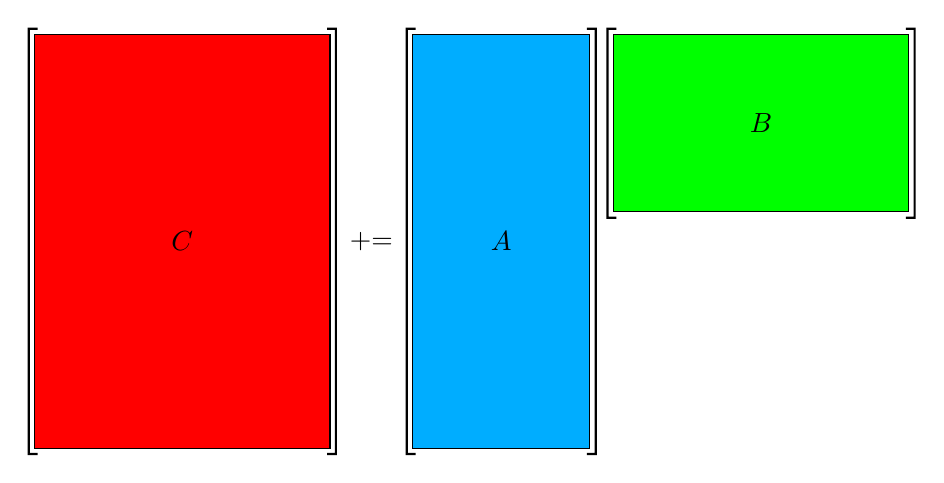
\begin{tikzpicture}[scale=0.75]
      \begin{scope}
        \tikzmat{0,0}{5, 7}
        \filldraw[fill=red] (0, 0) rectangle node {$C$} +(5, 7);
      \end{scope}
      \node at (5.7, 3.5) {+=};
      \begin{scope}[xshift=6.4cm]
        \tikzmat{0,0}{3, 7}
        \filldraw[fill=cyan] (0, 0) rectangle node[] {$A$} +(3, 7);
      \end{scope}
      \begin{scope}[xshift=9.8cm, yshift=4cm]
        \tikzmat{0,0}{5,3}
        \filldraw[fill=green] (0, 0) rectangle node {$B$} +(5, 3);
      \end{scope}

      
    \end{tikzpicture}
  \end{center}
\end{frame}

%%%%%%%%%%%%%%%%%%%%%%%%%%%%%%%%%%%%%%%%%%%%%%%%%%%%%%%%%%%%%%%%%%%%%%

\begin{frame}[label=gemm,fragile]
  \frametitle{Level-3 General Matrix-Matrix Product (\mintinline{C}{xGEMM})}

  \begin{center}
    \begin{tikzpicture}[scale=0.75]
      \path[use as bounding box] (-5, 0) rectangle (8, 11);
      \node[anchor=west] at (-5, 10) {$\displaystyle C_{ij} \gets C_{ij} + \sum_{k} A_{ik} B_{kj}$};
      \node[anchor=west] at (-5, 9) {$\displaystyle C_{ij} \gets C_{ij} + $ \mintinline{C}{xDOT(A[i,:], B[:,j])}};

      \begin{scope}[xshift=4cm] % C
        \tikzmat{0,0}{5, 7}
        \filldraw[fill=red] (0, 0) rectangle +(5, 7);
        \foreach \j in {0.5, 1, ..., 6.5} {
          \draw (0, \j) -- +(5, 0);
        }
        \foreach \i in {0.5, 1, ..., 4.5} {
          \draw (\i, 0) -- +(0, 7); 
        }
        % square blocks
        \foreach \j in {1, ..., 6} {
          \draw<2>[very thick] (0, \j) -- +(5, 0);
        }
        \foreach \i in {1, ..., 4} {
          \draw<2->[very thick] (\i, 0) -- +(0, 7); 
        }
        % rectangular blocks
        \foreach \j in {1, 2.5, ..., 6} {
          \draw<3->[very thick] (0, \j) -- +(5, 0); 
        }
        % mega square blocks
        \foreach \j in {1, 4} {
          \draw<4>[line width=1mm] (0, \j) -- +(5, 0); 
        }
        \foreach \i in {3} {
          \draw<4>[line width=1mm] (\i, 0) -- +(0, 7); 
        }
      \end{scope}

      \begin{scope} % A
        \tikzmat{0,0}{3, 7}
        \filldraw[fill=cyan] (0, 0) rectangle +(3, 7);
        \foreach \j in {0.5, 1, ..., 6.5} {
          \draw[] (0, \j) -- +(3, 0); 
        }
        % square blocks
        \foreach \j in {1, ..., 6} {
          \draw<2>[very thick] (0, \j) -- +(3, 0);
        }
        \foreach \i in {1, 2} {
          \draw<2->[very thick] (\i, 0) -- +(0, 7); 
        }
        % rectangular blocks
        \foreach \j in {1, 2.5, ..., 6} {
          \draw<3->[very thick] (0, \j) -- +(3, 0); 
        }
        % mega blocks
        \foreach \j in {1, 4} {
          \draw<4>[line width=1mm] (0, \j) -- +(3, 0); 
        }
      \end{scope}
      \begin{scope}[xshift=4cm, yshift=8cm] % B
        \tikzmat{0,0}{5,3}
        \filldraw[fill=green] (0, 0) rectangle +(5, 3);
        \foreach \i in {0.5, 1, ..., 4.5} {
          \draw (\i, 0) -- +(0, 3); 
        }
        % square blocks
        \foreach \j in {1, ..., 2} {
          \draw<2>[very thick] (0, \j) -- +(5, 0);
        }
        \foreach \i in {1, ..., 4} {
          \draw<2->[very thick] (\i, 0) -- +(0, 3); 
        }
        % rectangular blocks
        \foreach \j in {1.5} {
          \draw<3->[very thick] (0, \j) -- +(5, 0); 
        }
        % mega blocks
        \foreach \i in {3} {
          \draw<4>[line width=1mm] (\i, 0) -- +(0, 3); 
        }
      \end{scope}
    \end{tikzpicture}
  \end{center}

  \begin{textblock}{5}(0.75,6)
    \begin{block}{Algorithm for $P_{ij}$}
      \begin{itemize}
      \item Allgather $A[i,:]$ \\ on process row $i$
      \item Allgather $B[:,j]$ \\ on process col $j$
      \item \only<1>{\texttt{xDOT(...)}} \only<2,4>{\texttt{xGEMM(...)} \smiley} \only<3>{\sout{\texttt{xGEMM(...)}} \triste}
      \item<only@3> \sout{pipeline} \triste
      \item<only@2> Store 3 blocks \smiley
      \item<only@4> Store \alert{6} blocks
      \item<only@2,4> Pipeline \smiley
        \begin{itemize}
        \item<only@2,4> complex \triste
        \end{itemize}
      \item<only@1,3> \alert{Store full row/col}
      \end{itemize}
    \end{block}
  \end{textblock}
  
\end{frame}

%%%%%%%%%%%%%%%%%%%%%%%%%%%%%%%%%%%%%%%%%%%%%%%%%%%%%%%%%%%%%%%%%%%%%%%%%%%%

\begin{frame}[label=gemm]
  \frametitle{Level-3 General Matrix-Matrix Product (\mintinline{C}{xGEMM})}


  \begin{textblock}{5}(0.75,7)
    \begin{block}{Algorithm for $P_{ij}$}
      \begin{itemize}
      \item<only@1,2> Repeat $k$ times:
      \item<only@3-> Repeat $k / \alert{b}$ times:
      \item Broadcast $A[:,k]$ 
      \item Broadcast $B[k,:]$ 
      \item \only<1,2>{\mintinline{C}{xGER(...)}} \only<3->{\mintinline{C}{xGEMM(...)} \smiley}
      \item Pipeline \smiley
        \begin{itemize}
        \item Simpler \smiley
        \end{itemize}
      \end{itemize}
    \end{block}
  \end{textblock}
  
  
  \begin{center}
    \begin{tikzpicture}[scale=0.75]
      \path[use as bounding box] (-5, 0) rectangle (8, 11);
      \node[anchor=west] at (-5, 10) {$\displaystyle C \gets C + \sum_{k} A_{k} B_{k}$};
      \node[anchor=west] at (-5, 9) {$\displaystyle C \gets C + $ \mintinline{C}{xGER(A[:,k], B[k:])}};

      \begin{scope}[xshift=4cm] % C
        \tikzmat{0,0}{5, 7}
        \filldraw[fill=red] (0, 0) rectangle +(5, 7);
        % % rectangular blocks
        % \foreach \i in {1, ..., 4} {
        %   \draw<3->[very thick] (\i, 0) -- +(0, 7); 
        % }
        % \foreach \j in {1, 2, ..., 6} {
        %   \draw<3,4>[very thick] (0, \j) -- +(5, 0); 
        % }
        % \foreach \j in {1, 2.5, ..., 6} {
        %   \draw<5>[very thick] (0, \j) -- +(5, 0); 
        % }
        % % mega square blocks
        % \foreach \j in {1, 4} {
        %   \draw<5>[line width=1mm] (0, \j) -- +(5, 0); 
        % }
        % \foreach \i in {3} {
        %   \draw<5>[line width=1mm] (\i, 0) -- +(0, 7); 
        % }
      \end{scope}

      \begin{scope}[] % A
        \tikzmat{0,0}{3, 7}
        \filldraw<1,3,5>[fill=cyan] (0, 0) rectangle +(3, 7);
        \filldraw<2>[fill=cyan] (0, 0) rectangle +(0.5, 7);
        \filldraw<2>[fill=cyan,nearly transparent] (0.5, 0) rectangle +(2.5, 7);
        \filldraw<4>[fill=cyan] (0, 0) rectangle +(1, 7);
        \filldraw<4>[fill=cyan,nearly transparent] (1, 0) rectangle +(2, 7);

        \foreach \i in {0.5, 1, ..., 2.5} {
          \draw (\i, 0) -- +(0, 7); 
        }
        % rectangular blocks
        \foreach \i in {1, 2} {
          \draw<3->[very thick] (\i, 0) -- +(0, 7); 
        }
        \foreach \j in {1, 2, ..., 6} {
          \draw<3,4>[very thick] (0, \j) -- +(3, 0); 
        }
        \foreach \j in {1, 2.5, ..., 6} {
          \draw<5>[very thick] (0, \j) -- +(3, 0); 
        }
        % mega blocks
        \foreach \j in {1, 4} {
          \draw<5>[line width=1mm] (0, \j) -- +(3, 0); 
        }
      \end{scope}

      \begin{scope}[xshift=4cm, yshift=8cm] % B
        \tikzmat{0,0}{5,3}
        \filldraw<1,3,5>[fill=green] (0, 0) rectangle +(5, 3);
        \filldraw<2>[fill=green] (0, 2.5) rectangle +(5, 0.5);
        \filldraw<2>[fill=green, nearly transparent] (0, 0) rectangle +(5, 2.5);
        \filldraw<4>[fill=green] (0, 2) rectangle +(5, 1);
        \filldraw<4>[fill=green, nearly transparent] (0, 0) rectangle +(5, 2);
        \foreach \j in {0.5, 1, ..., 2.5} {
          \draw (0, \j) -- +(5, 0); 
        }
        % rectangular blocks
        \foreach \i in {1, ..., 4} {
          \draw<3->[very thick] (\i, 0) -- +(0, 3); 
        }
        \foreach \j in {1, 2} {
          \draw<3,4>[very thick] (0, \j) -- +(5, 0); 
        }
        \foreach \j in {1.5} {
          \draw<5>[very thick] (0, \j) -- +(5, 0); 
        }
        % mega blocks
        \foreach \i in {3} {
          \draw<5>[line width=1mm] (\i, 0) -- +(0, 3); 
        }      \end{scope}

      % bcast
      \foreach \i in {1.5, 3.5, 5.5} {
        \draw<2>[cyan,ultra thick,->] (0.5, \i) -- +(8 - 0.6*\i, 0); 
        \draw<4>[cyan,ultra thick,->] (1, \i) -- +(7.5 - 0.6*\i, 0); 
      }
      \foreach \i in {0.5, 2.5, 4.5} {
        \draw<2>[green,ultra thick,->] (4+\i, 10.5) -- +(0, -3.5 - 1.25*\i); 
        \draw<4>[green,ultra thick,->] (4+\i, 10) -- +(0, -3 - 1.25*\i); 
      }
    \end{tikzpicture}
  \end{center}
\end{frame}



% \begin{frame}[label=gemm]
%   \frametitle{Level-3 General Matrix-Matrix Product (\mintinline{C}{xGEMM})}

%   \begin{center}
%     \begin{tikzpicture}[scale=0.75]
%       \begin{scope}[xshift=4cm]
%         \tikzmat{0,0}{5, 7}

%         \begin{scope}
%           \clip (0, 0) rectangle +(5, 7);
%           \foreach \i in {0, 2, 4, 6} {
%             \foreach \j in {0, 3, 6} {
%               \filldraw[fill=red]             (\i,   \j)   rectangle +(1, 1);
%               \filldraw[fill=red!50!white]    (\i,   \j+1) rectangle +(1, 1);
%               \filldraw[fill=orange]          (\i  , \j+2) rectangle +(1, 1);
%               \filldraw[fill=orange!50!white] (\i+1, \j)   rectangle +(1, 1);
%               \filldraw[fill=yellow]          (\i+1, \j+1) rectangle +(1, 1);
%               \filldraw[fill=yellow!50!white] (\i+1, \j+2) rectangle +(1, 1);
%             }
%           }
%         \end{scope}
%         \foreach \j in {0.5, 1, ..., 6.5} {
%           \draw (0, \j) -- +(5, 0);
%         }
%         \foreach \i in {0.5, 1, ..., 4.5} {
%           \draw (\i, 0) -- +(0, 7); 
%         }
%       \end{scope}

%       \begin{scope}[]
%         \tikzmat{0,0}{3, 7}
%         \begin{scope}
%           \clip (0, 0) rectangle +(3, 7);
%           \foreach \i in {0, 2, 4, 6} {
%             \foreach \j in {0, 3, 6} {
%               \filldraw[fill=blue]          (\i,   \j)   rectangle +(1, 1);
%               \filldraw[fill=blue!50!white] (\i,   \j+1) rectangle +(1, 1);
%               \filldraw[fill=teal]          (\i,   \j+2) rectangle +(1, 1);
%               \filldraw[fill=teal!50!white] (\i+1, \j)   rectangle +(1, 1);
%               \filldraw[fill=cyan]          (\i+1, \j+1) rectangle +(1, 1);
%               \filldraw[fill=cyan!50!white] (\i+1, \j+2) rectangle +(1, 1);
%             }
%           }
%         \end{scope}
%         \foreach \i in {0.5, 1, ..., 2.5} {
%           \draw (\i, 0) -- +(0, 7);
%         }        
%         \foreach \j in {0.5, 1, ..., 6.5} {
%           \draw (0, \j) -- +(3, 0); 
%         }
%       \end{scope}
%       \begin{scope}[xshift=4cm, yshift=8cm]
%         \tikzmat{0,0}{5,3}
%         \begin{scope}
%           \clip (0, 0) rectangle +(5, 3);
%           \foreach \i in {0, 2, 4, 6} {
%             \foreach \j in {0, 3, 6} {
%               \filldraw[fill=green]              (\i,   \j)   rectangle +(1, 1);
%               \filldraw[fill=green!50!white]     (\i,   \j+1) rectangle +(1, 1);
%               \filldraw[fill=lime]               (\i,   \j+2) rectangle +(1, 1);
%               \filldraw[fill=lime!50!white]      (\i+1, \j)   rectangle +(1, 1);
%               \filldraw[fill=lightgray]          (\i+1, \j+1) rectangle +(1, 1);
%               \filldraw[fill=lightgray!50!white] (\i+1, \j+2) rectangle +(1, 1);
%             }
%           }
%         \end{scope}
%         \foreach \i in {0.5, 1, ..., 4.5} {
%           \draw (\i, 0) -- +(0, 3); 
%         }
%         \foreach \j in {0.5, 1, ..., 2.5} {
%           \draw (0, \j) -- +(5, 0); 
%         }
%       \end{scope}
      
%     \end{tikzpicture}
%   \end{center}
% \end{frame}

%%%%%%%%%%%%%%%%%%%%%%%%%%%%%%%%%%%%%%%%%%%%%%%%%%%%%%%%%%%%%%%%%%%%%

% \begin{frame}[label=gemm]
%   \frametitle{Level-3 General Matrix-Matrix Product (\mintinline{C}{xGEMM})}

%   \begin{center}
%     \begin{tikzpicture}[scale=0.75]
%       \draw<2>[dashed] (0.5, 7) |- (4, 10.5);
%       \draw<2>[dashed] (1.5, 7) |- (4, 9.5);
%       \draw<2>[dashed] (2.5, 7) |- (4, 8.5);

%       \begin{scope}[xshift=4cm]
%         \tikzmat{0,0}{5, 7}

%         \begin{scope}
%           \clip (0, 0) rectangle +(5, 7);
%           \foreach \i in {0, 2, 4, 6} {
%             \foreach \j in {0, 3, 6} {
%               \filldraw[fill=red]             (\i,   \j)   rectangle +(1, 1);
%               \filldraw<1>[fill=red!50!white]    (\i,   \j+1) rectangle +(1, 1);
%               \filldraw<1>[fill=orange]          (\i  , \j+2) rectangle +(1, 1);
%               \filldraw<1>[fill=orange!50!white] (\i+1, \j)   rectangle +(1, 1);
%               \filldraw<1>[fill=yellow]          (\i+1, \j+1) rectangle +(1, 1);
%               \filldraw<1>[fill=yellow!50!white] (\i+1, \j+2) rectangle +(1, 1);
%             }
%           }
%         \end{scope}
%         \foreach \j in {0.5, 1, ..., 6.5} {
%           \draw (0, \j) -- +(5, 0);
%         }
%         \foreach \i in {0.5, 1, ..., 4.5} {
%           \draw (\i, 0) -- +(0, 7); 
%         }
%       \end{scope}

%       \begin{scope}[]
%         \tikzmat{0,0}{3, 7}
%         \begin{scope}
%           \clip (0, 0) rectangle +(3, 7);
%           \foreach \i in {0, 2, 4, 6} {
%             \foreach \j in {0, 3, 6} {
%               \filldraw[fill=blue]          (\i,   \j)   rectangle +(1, 1);
%               \filldraw<1>[fill=blue!50!white] (\i,   \j+1) rectangle +(1, 1);
%               \filldraw<1>[fill=teal]          (\i,   \j+2) rectangle +(1, 1);
%               \filldraw<1>[fill=teal!50!white] (\i+1, \j)   rectangle +(1, 1);
%               \filldraw<1>[fill=cyan]          (\i+1, \j+1) rectangle +(1, 1);
%               \filldraw<1>[fill=cyan!50!white] (\i+1, \j+2) rectangle +(1, 1);
%             }
%           }
%         \end{scope}
%         \filldraw<2>[fill=blue!50!white,opacity=0.1] (1, 6) rectangle +(1, 1);

%         \foreach \i in {0.5, 1, ..., 2.5} {
%           \draw (\i, 0) -- +(0, 7);
%         }        
%         \foreach \j in {0.5, 1, ..., 6.5} {
%           \draw (0, \j) -- +(3, 0); 
%         }
%       \end{scope}
%       \begin{scope}[xshift=4cm, yshift=8cm]
%         \tikzmat{0,0}{5,3}
%         \begin{scope}
%           \clip (0, 0) rectangle +(5, 3);
%           \foreach \i in {0, 2, 4, 6} {
%             \foreach \j in {0, 3, 6} {
%               \filldraw<1>[fill=green]              (\i,   \j)   rectangle +(1, 1);
%               \filldraw<1>[fill=green!50!white]     (\i,   \j+1) rectangle +(1, 1);
%               \filldraw[fill=lime]               (\i,   \j+2) rectangle +(1, 1);
%               \filldraw<1>[fill=lime!50!white]      (\i+1, \j)   rectangle +(1, 1);
%               \filldraw<1>[fill=lightgray]          (\i+1, \j+1) rectangle +(1, 1);
%               \filldraw<1>[fill=lightgray!50!white] (\i+1, \j+2) rectangle +(1, 1);
%             }
%           }
%         \end{scope}
%         \filldraw<2>[fill=green,opacity=0.1]             (0,   0)   rectangle +(1, 1);
%         \filldraw<2>[fill=green!50!white,opacity=0.1]     (0,   1) rectangle +(1, 1);

%         \foreach \i in {0.5, 1, ..., 4.5} {
%           \draw (\i, 0) -- +(0, 3); 
%         }
%         \foreach \j in {0.5, 1, ..., 2.5} {
%           \draw (0, \j) -- +(5, 0); 
%         }
%       \end{scope}
      
%     \end{tikzpicture}
%   \end{center}
% \end{frame}


%%%%%%%%%%%%%%%%%%%%%%%%%%%%%%%%%%%%%%%%%%%%%%%%%%%%%%%%%%%%%%%%%%%%%%

\subsubsection{TRSM}

\begin{frame}[label=trsm,fragile]
  \frametitle{Level-3 Triangular Solve (\mintinline{C}{xTRSM})}

  \begin{center}
      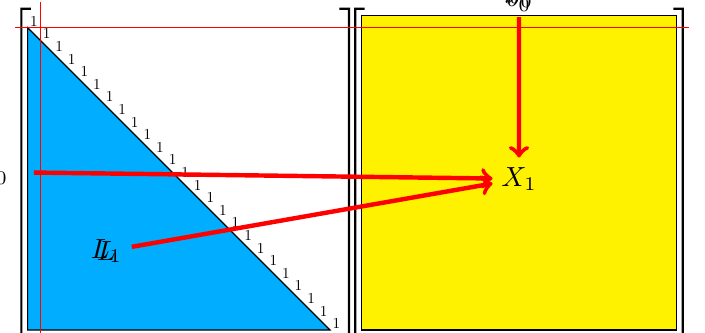
\begin{tikzpicture}[scale=0.8]
        \useasboundingbox (-5.3, 0.4) rectangle (5, 4.8);

        \begin{scope}[xshift=-5.3cm]
          \tikzmat{0,0}{5,5}
          \filldraw[fill=cyan] (0, 0) -- (0, 4.8) -- (4.8, 0) -- cycle;
          \foreach \i in {0, 0.2, ..., 4.8} {
            \path (\i,4.8-\i) rectangle node {\scalebox{0.55}{1}} +(0.2,0.2);
          }
          
          \node<1> at (1.25, 1.25) {$L$};

          \coordinate (l0) at (0.1, 2.5);
          \node<2-> at (-0.5, 2.5) {$\ell_0$};
          \node<2-> at (1.25, 1.25)  (l1) {$L_{1}$};
          
          % découpage rouge
          \draw<2->[red] (-0.2, 4.8) -- +(5.4, 0);
          \draw<2->[red] (0.2, -0.2) -- +(0, 5.4);
        \end{scope}

        
        \tikzmat{0,0}{5,5}
        \filldraw[fill=Gray!70] (0, 0) rectangle (5,5);

        \node<1> at (2.5, 2.5) {$B$};
        \node<2> at (2.5, 5.25) (b0) {$b_{0}$};
        \node<3-> at (2.5, 5.25) (x0) {$x_{0}$};

        \node<2-3> at (2.5, 2.4)  (b1) {$B_{1}$};
        \node<5> at (2.5, 2.4) (b) {$B_{1} - \ell_{0} x_{0}$};
        
        \draw<4>[pattern=north west lines] (0, 0) rectangle +(5, 4.8);
        \draw<6>[pattern=north west lines] (0, 0) rectangle +(5, 4.8);
        
        \filldraw<3->[fill=yellow] (0, 4.8) rectangle +(5, 0.2);
        \filldraw<7->[fill=yellow] (0, 0) rectangle +(5, 4.8);

        \node<7-> at (2.5, 2.4) (x1) {$X_{1}$};
                
        % découpage rouge
        \draw<2->[red] (-0.2, 4.8) -- +(5.4, 0);

        % GER
        \draw<4>[red,ultra thick, ->] (x0) edge (b1);    
        \draw<4>[red,ultra thick] (l0) edge[->] (b1);

        % appel récursif
        \draw<6>[red,ultra thick, ->] (l1) edge (b1);    
      \end{tikzpicture}
    \end{center}
    
  \begin{columns}
    \begin{column}{5cm}
\[
     \begin{pmatrix}
       1 &  \\
       \ell_{0} & L_{1} 
     \end{pmatrix}
     \begin{pmatrix}
       x_{0} \\
       X_{1}  
     \end{pmatrix}
     =
     \begin{pmatrix}
     b_{0} \\
     B_{1} \\
   \end{pmatrix}
 \]

   \vspace{-0.5cm}
   
   \begin{align*}     
     x_{0} &= b_{0} \\
     L_{1} X_1 &= B_{1} - \ell_{0} x_{0}
   \end{align*}
      
    \end{column}
    \begin{column}{5.5cm}

 \begin{block}{\emph{Iterative} algorithm}
   \begin{enumerate}
   \item<4-> $B_{1} \gets B_{1} - \ell_{0} x_{0}$
     \begin{itemize}
     \item level-2 \mintinline{C}{xGER}
     \end{itemize}
     
   \item<6-> Solve $L_{1} X_1 = B_{1} - \ell_{0} x_{0}$
     \begin{itemize}
     \item level-3 \mintinline{C}{xTRSM}
     \end{itemize}
   \end{enumerate}
 \end{block}

\end{column}
\end{columns}
\end{frame}

%%%%%%%%%%%%%%%%%%%%%%%%%%%%%%%%%%%%%%%%%%%%%%%%%%%%%%%%%%%%%%%%%%%%%%%%

\begin{frame}[label=trsm,fragile]
  \frametitle{Level-3 Triangular Solve (\mintinline{C}{xTRSM})}
  \framesubtitle{Complexity Analysis}
  
  \begin{itemize}
  \item \mintinline{C}{xGER} runs in time $T_{ger} \leq \alpha m n$.
  \item \mintinline{C}{xTRSM(m, n) == xGER(m, n) + ... + xGER(1, n)}
  \item $T_{trsm} \leq \frac{\alpha}{2} m^2 n$
  \end{itemize}

\end{frame}

%%%%%%%%%%%%%%%%%%%%%%%%%%%%%%%%%%%%%%%%%%%%%%%%%%%%%%%%%%%%%%%%%%%%%%%% 

\begin{frame}[label=trsm]
  \frametitle{\textbf{Blocked} Level-3 Triangular Solve  (\mintinline{C}{xTRSM})}

  \begin{center}
      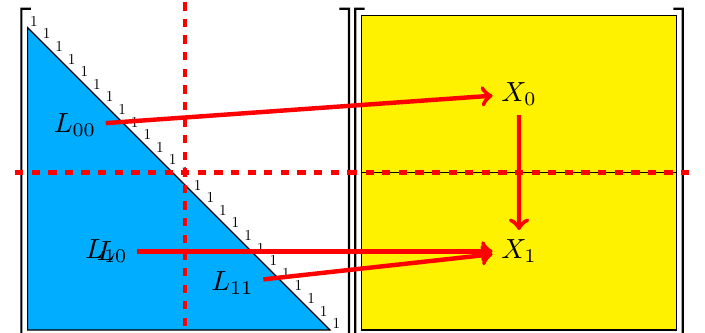
\begin{tikzpicture}[scale=0.8]
        \useasboundingbox (-5.3, 0.4) rectangle (5, 4.8);

        \begin{scope}[xshift=-5.3cm]
          \tikzmat{0,0}{5,5}
          \filldraw[fill=cyan] (0, 0) -- (0, 4.8) -- (4.8, 0) -- cycle;
          \foreach \i in {0, 0.2, ..., 4.8} {
            \path (\i,4.8-\i) rectangle node {\scalebox{0.55}{1}} +(0.2,0.2);
          }
          
          \node<1> at (1.25, 1.25) {$L$};

          \node<2-> at (1.25, 1.25) (l10) {$L_{10}$};
          \node<2-> at (0.75, 3.25) (l00) {$L_{00}$};
          \node<2-> at (3.25, 0.75)  (l11) {$L_{11}$};
          
          % découpage rouge
          \draw<2->[red, ultra thick, dashed] (-0.2, 2.5) -- (5.2, 2.5);
          \draw<2->[red, ultra thick, dashed] (2.5, -0.2) -- (2.5, 5.2);
        \end{scope}

        
        \tikzmat{0,0}{5,5}
        \filldraw[fill=Gray!70] (0, 0) rectangle (5,5);

        \node<1> at (2.5, 2.5) {$B$};
        
%        \coordinate (b0) at (2.5, 3.75) ;
        \node<2> at (2.5, 3.75) (b0) {$B_{0}$};
        
%        \node (b1) at (2.5, 1.25) {};
        \node<2-4> at (2.5, 1.25)  (b1) {$B_{1}$};
        \node<6> at (2.5, 1.25) (b) {$B_{1} - L_{10} X_{0}$};
        
        \draw<3>[pattern=north west lines] (0, 2.5) rectangle +(5, 2.5);
        \draw<5>[pattern=north west lines] (0, 0) rectangle +(5, 2.5);
        \draw<7>[pattern=north west lines] (0, 0) rectangle +(5, 2.5);
        
        \filldraw<4->[fill=yellow] (0, 2.5) rectangle +(5, 2.5);
        \filldraw<8->[fill=yellow] (0, 0) rectangle +(5, 2.5);

        \node<4-> at (2.5, 3.75) (x0) {$X_{0}$};
        \node<8-> at (2.5, 1.25) (x1) {$X_{1}$};
                
        % découpage rouge
        \draw<2->[red, ultra thick, dashed] (-0.2, 2.5) -- (5.2, 2.5);

        % 1er appel récursif
        \draw<3>[red,ultra thick, ->] (l00) edge (b0);    

        % GEMM
        \draw<5>[red,ultra thick, ->] (x0) edge (b1);    
        \draw<5>[red,ultra thick, ->] (l10) edge (b1);

        % 2ème appel récursif
        \draw<7>[red,ultra thick, ->] (l11) edge (b1);    
      \end{tikzpicture}
    \end{center}
    
  \begin{columns}
    \begin{column}{5cm}
\[
     \begin{pmatrix}
       L_{00} &  \\
       L_{10} & L_{11} 
     \end{pmatrix}
     \begin{pmatrix}
       X_{0} \\
       X_{1}  
     \end{pmatrix}
     =
     \begin{pmatrix}
     B_{0} \\
     B_{1} \\
   \end{pmatrix}
 \]

   \vspace{-0.5cm}
   
   \begin{align*}     
     L_{00} X_{0} &= B_{0} \\
     L_{11} X_1 &= B_{1} - L_{10} X_{0}
   \end{align*}
      
    \end{column}
    \begin{column}{5.5cm}

 \begin{block}{\emph{Blocked} algorithm}
   \begin{enumerate}
   \item<3-> Solve $L_{00} X_{0} = B_{0}$
     \begin{itemize}
     \item level-3 \texttt{TRSM}
     \end{itemize}

   \item<5-> $B_{1} \gets B_{1} - L_{10} X_{0}$
     \begin{itemize}
     \item level-3 \texttt{GEMM}
     \end{itemize}
     
   \item<7-> Solve $L_{11} X_1 = B_{1} - L_{10} X_{0}$
     \begin{itemize}
     \item level-3 \texttt{TRSM}
     \end{itemize}
   \end{enumerate}
 \end{block}

\end{column}
\end{columns}

\end{frame}

%%%%%%%%%%%%%%%%%%%%%%%%%%%%%%%%%%%%%%%%%%%%%%%%%%%%%%%%%%%%%%%%%%%%%%%%

\begin{frame}[label=trsm,fragile]
  \frametitle{\textbf{Blocked} Level-3 Triangular Solve (\mintinline{C}{xTRSM})}
  \framesubtitle{Complexity Analysis}
  
  \begin{itemize}
  \item \mintinline{C}{xGER} runs in time $T_{ger} \leq \alpha m n$
  \item \mintinline{C}{xGEMM} runs in time $T_{gemm} \leq \beta m n k$
  \item (unblocked) \mintinline{C}{xTRSM(m, n)} runs in time $T \leq \alpha m^2 n / 2$
  \item If $m \leq m_0$, use unblocked algorithm \hfill (too small)
    \begin{itemize}
    \item $T_{m} = \frac{\alpha}{2} {m}^2 n$
    \end{itemize}

  \item Otherwise, use recursive blocked algorithm
    \begin{itemize}
    \item $T_{m} = 2 T_{m/2} + \beta\left(\frac{m}{2}\right)^2 n + \bigO{1}$
    \end{itemize}

  \end{itemize}

  \begin{block}{Asymptotic performance}
    \begin{itemize}
    \item Assume $T_m = \gamma m^2 n$ \hfill (as in unblocked case)
    \item $\gamma m^2 n = 2\gamma\left(\frac{m}{2}\right)^2 n + \beta\left(\frac{m}{2}\right)^2 n + \bigO{1}$
    \item $\gamma = \beta / 2$ \hfill (for large $m$)
    \end{itemize}
  \end{block}
  
\end{frame}


\subsubsection{LAPACK and LU}

%%%%%%%%%%%%%%%%%%%%%%%%%%%%%%%%%%%%%%%%%%%%%%%%%%%%%%%%%%%%%%%%%%%%%%%%%%%%%%%%%%%%%%%%%

\begin{frame}[label=lapack]
  \frametitle{Solving Actual Problems}

  \begin{center}
    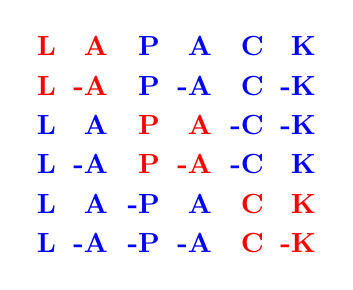
\begin{tikzpicture}[yscale=0.5,xscale=0.66,every node/.style={anchor=south east,font=\bfseries}]
      \node[red] at (0, 5) {L};
      \node[red] at (0, 4) {L};
      \node[blue] at (0, 3) {L};
      \node[blue] at (0, 1) {L};
      \node[blue] at (0, 0) {L};
      \node[blue] at (0, 2) {L};
      
      \node[red] at (1, 5) {A};
      \node[red] at (1, 4) {-A};
      \node[blue]  at (1, 3) {A};
      \node[blue]  at (1, 2) {-A};
      \node[blue] at (1, 1) {A};
      \node[blue] at (1, 0) {-A};

      \node[blue]  at (2, 5) {P};
      \node[blue]  at (2, 4) {P};
      \node[red] at (2, 3) {P};
      \node[red] at (2, 2) {P};
      \node[blue] at (2, 1) {-P};
      \node[blue] at (2, 0) {-P};

      \node[blue]  at (3, 5) {A};
      \node[blue]  at (3, 4) {-A};
      \node[red] at (3, 3) {A};
      \node[red] at (3, 2) {-A};
      \node[blue] at (3, 1) {A};
      \node[blue] at (3, 0) {-A};

      \node[blue] at (4, 5) {C};
      \node[blue] at (4, 4) {C};
      \node[blue] at (4, 3) {-C};
      \node[blue]  at (4, 2) {-C};
      \node[red]  at (4, 1) {C};
      \node[red] at (4, 0) {C};

      \node[blue] at (5, 5) {K};
      \node[blue] at (5, 4) {-K};
      \node[blue] at (5, 3) {-K};
      \node[blue]  at (5, 2) {K};
      \node[red]  at (5, 1) {K};
      \node[red] at (5, 0) {-K};

    \end{tikzpicture}
  \end{center}
  
  \begin{exampleblock}{\textbf{LAPACK}: Linear Algebra PACKage}
    \begin{itemize}
    \item Development started in the 1990's (still active)
    \item Built upon the BLAS (Fortran: \alert{column-major})
    \item Solve linear systems, least-squares, eigenvalues, etc.
    \item \textbf{Main algorithmic idea}: \red{use level-3 BLAS}
      \begin{itemize}
      \item High \red{arithmetic intensity}
      \item Significant performance gain over naive code
      \end{itemize}
    \end{itemize}
  \end{exampleblock}  
\end{frame}

%%%%%%%%%%%%%%%%%%%%%%%%%%%%%%%%%%%%%%%%%%%%%%%%


\begin{frame}[label=lu,fragile=singleslide]
  \frametitle{LU Factorization}

  \begin{center}
    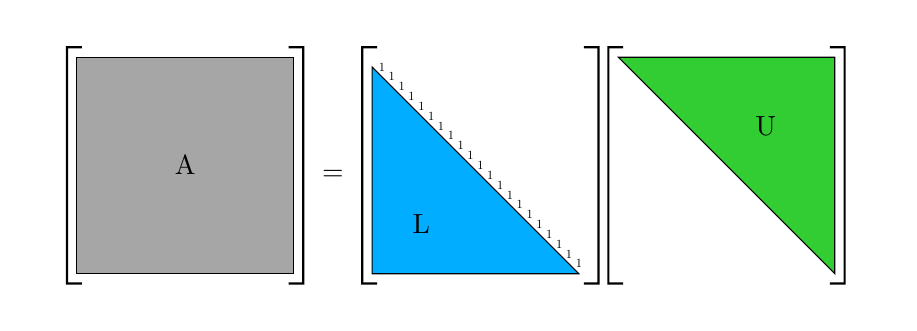
\begin{tikzpicture}[scale=1.25]
      \useasboundingbox (-0.5,-0.3) rectangle (8.25,2.5);
      
      % L en haut
      \begin{scope}[xshift=3cm]
        \tikzmat{0,0}{2.2,2.2}
        \foreach \i in {0, 0.1, ..., 2.1}
        \path (\i,2-\i) rectangle node {\scalebox{0.45}{1}} +(0.2,0.2);
        \filldraw[fill=cyan] (0,0) -- ++(0, 2.1)  -- ++(2.1,-2.1) -- cycle;
        \node at (0.5, 0.5) {L};
      \end{scope}
      
      % U en haut
      \begin{scope}[xshift=5.5cm]
        \tikzmat{0,0}{2.2,2.2}
        \draw[fill=LimeGreen] (0,2.2) -- ++(2.2,0) -- ++(0,-2.2) -- cycle;
        \node at (1.5, 1.5) {U};
      \end{scope}
      
      \node at (2.6,1) {$=$};
    
      % matrice grise en haut
      \begin{scope}[xshift=0cm]
        \tikzmat{0,0}{2.2,2.2}
        \filldraw[fill=Gray!70] (0,0) rectangle node{A} +(2.2,2.2);
      \end{scope}
    \end{tikzpicture}
  \end{center}

  \bigskip
  
  \begin{itemize}
  \item   Main tool to solve $Ax = b$ when $A$ is invertible
  \item \textbf{DISCLAIMER}:
    \begin{itemize}
    \item This presentation ignores \alert{pivoting}
    \item \alert{Pivoting} is required for numerical stability
    \item In parallel, \alert{pivoting} is a pain in the \verb|[---REDACTED---]|
    \end{itemize}
  \end{itemize}


\end{frame}

%%%%%%%%%%%%%%%%%%%%%%%%%%%%%%%%%%%%%%%%%%%%%%%%%%%%%%%%%%

\begin{frame}[label=lu]
  \frametitle{LU Factorization}
%  \framesubtitle{Right-looking Algorithm}

  \begin{columns}
    \begin{column}{5cm}
      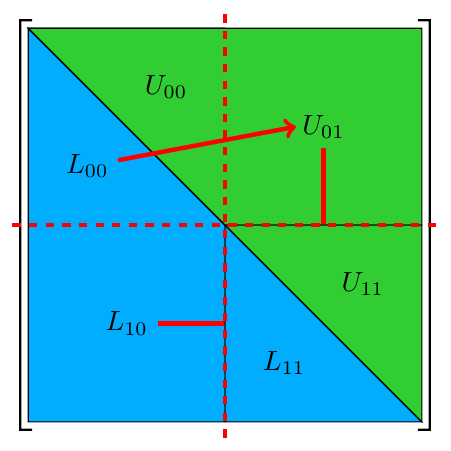
\begin{tikzpicture}
        \draw[red,dotted,use as bounding box] (0, 0) rectangle (5, 5);
    \tikzmat{0,0}{5,5}
    \filldraw[fill=Gray!70] (0, 0) rectangle (5,5);

    \node<1> at (2.5, 2.5) {$A$};

    \node<2> at (1.25, 3.75) {$A_{00}$};
    \node<2> at (1.25, 1.25) {$A_{10}$};

    \node<2-6> at (3.75, 1.25) (a11) {$A_{11}$};
    \node<8> at (3.75, 1.25) (b) {$A_{11} - L_{10} U_{01}$};

    \node<2-4> at (3.75, 3.75) {$A_{01}$};

    \draw<3>[pattern=north west lines] (0,0) rectangle +(2.5, 5);
    \draw<5>[pattern=north west lines] (2.5, 2.5) rectangle +(2.5, 2.5);
    \draw<7,9>[pattern=north west lines] (2.5 , 0) rectangle +(2.5, 2.5);
    
    \filldraw<4->[fill=cyan] (0,5) -- ++(2.5, -2.5) -- (2.5, 0) -- (0, 0) -- cycle;
    \filldraw<4-5>[fill=LimeGreen] (0,5) -- (2.5, 2.5) -- (2.5, 5) -- cycle;
    \filldraw<6->[fill=LimeGreen] (0,5) -- ++(5, 0) -- (5, 2.5) -- (2.5, 2.5) -- cycle;
    
    \node<4-> at (1.25, 1.25) (l10) {$L_{10}$};
    \node<4-> at (0.75, 3.25) (l00) {$L_{00}$};
    \node<4-> at (1.75, 4.25) {$U_{00}$};
    \node<6-> at (3.75, 3.75) (u01) {$U_{01}$};

    \draw<5>[red,ultra thick, ->] (l00) edge (3.4, 3.75);    
    \draw<7>[red,ultra thick, ->] (u01) edge (a11);    
    \draw<7>[red,ultra thick, ->] (l10) edge (a11);    

    
    \filldraw<10>[fill=cyan] (2.5, 2.5) -- (5, 0) -- (2.5, 0) -- cycle;
    \filldraw<10>[fill=LimeGreen] (2.5, 2.5) -- (5, 2.5) -- (5, 0) -- cycle;
    \node<10> at (3.25, 0.75) {$L_{11}$};
    \node<10> at (4.25, 1.75) {$U_{11}$};


      \draw<2->[red, ultra thick, dashed] (-0.2, 2.5) -- (5.2, 2.5);
      \draw<2->[red, ultra thick, dashed] (2.5, -0.2) -- (2.5, 5.2);
  \end{tikzpicture}
\end{column}
\begin{column}{5.5cm}

 \begin{block}{Recursive algorithm}
   \begin{enumerate}
   \item<3-> Factorize left half
   \item<5-> Solve $L_{00} U_{01} = A_{01}$
     \begin{itemize}
     \item level-3 \texttt{TRSM}
     \end{itemize}
     
   \item<7-> $A_{11} \gets A_{11} - L_{10} U_{01}$
     \begin{itemize}
     \item level-3 \texttt{GEMM}
     \end{itemize}
   \item<9-> Factorize $A_{11} - L_{10} U_{01}$
     
   \end{enumerate}
 \end{block}

\end{column}
\end{columns}

\medskip

\begin{visibleenv}<2->
\[
  \begin{pmatrix}
       A_{00} & A_{01} \\
       A_{10} & A_{11} 
     \end{pmatrix}
     =
     \begin{pmatrix}
       L_{00} &  \\
       L_{10} & L_{11} 
     \end{pmatrix}
     \begin{pmatrix}
       U_{00} & U_{01} \\
       & U_{11} 
     \end{pmatrix}
   \]

   \vspace{-0.5cm}
   
   \begin{align*}     
     L_{00} U_{01} &= A_{01} \\
     L_{11} U_{11} &= A_{11} - L_{10} U_{01}
   \end{align*}
 \end{visibleenv}
\end{frame}


%%%%%%%%%%%%%%%%%%%%%%%%%%%%%%%%%%%%%%%%%%%%%%%%%%%%%%%%%%%%%%%%%%%%%%%

\begin{frame}[label=sca-lu]
  \frametitle{Distributed LU Factorization}

  \begin{columns}
    \begin{column}{5cm}
  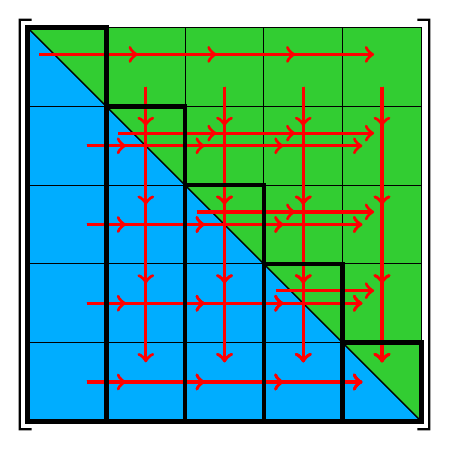
\begin{tikzpicture}
    \path[red,dotted,use as bounding box] (0, 0) rectangle (5, 5);
    \tikzmat{0,0}{5,5}
    \filldraw[fill=Gray!70] (0, 0) rectangle (5,5);

    % 2nd column gets ready
    \draw<7->[pattern=north west lines] (1, 3) rectangle +(1, 1);
    \draw<9->[pattern=north west lines] (1, 2) rectangle +(1, 1);
    \draw<9->[pattern=north west lines] (2, 3) rectangle +(1, 1);

    \draw<9->[pattern=north west lines] (2, 3) rectangle +(1, 1);
    \draw<11->[pattern=north west lines] (1, 1) rectangle +(1, 1);
    \draw<11->[pattern=north west lines] (2, 2) rectangle +(1, 1);
    \draw<11->[pattern=north west lines] (3, 3) rectangle +(1, 1);
    \draw<11->[pattern=north west lines] (3, 3) rectangle +(1, 1);

    \draw<13->[pattern=north west lines] (4, 3) rectangle +(1, 1);
    \draw<13->[pattern=north west lines] (3, 2) rectangle +(1, 1);
    \draw<13->[pattern=north west lines] (2, 1) rectangle +(1, 1);
    \draw<13->[pattern=north west lines] (1, 0) rectangle +(1, 1);

    \draw<15->[pattern=north west lines] (2, 0) rectangle +(1, 1);
    \draw<15->[pattern=north west lines] (3, 1) rectangle +(1, 1);
    \draw<15->[pattern=north west lines] (4, 2) rectangle +(1, 1);

    \draw<17->[pattern=north west lines] (3, 0) rectangle +(1, 1);
    \draw<17->[pattern=north west lines] (4, 1) rectangle +(1, 1);

    \draw<19->[pattern=north west lines] (4, 0) rectangle +(1, 1);

    % 2nd wave
    \draw<19->[pattern=north east lines] (2, 2) rectangle +(1, 1);

    \draw<21->[pattern=north east lines] (3, 2) rectangle +(1, 1);
    \draw<21->[pattern=north east lines] (2, 1) rectangle +(1, 1);

    \draw<23->[pattern=north east lines] (2, 0) rectangle +(1, 1);
    \draw<23->[pattern=north east lines] (3, 1) rectangle +(1, 1);
    \draw<23->[pattern=north east lines] (4, 2) rectangle +(1, 1);

    \draw<25->[pattern=north east lines] (3, 0) rectangle +(1, 1);
    \draw<25->[pattern=north east lines] (4, 1) rectangle +(1, 1);
    
    \draw<27->[pattern=north east lines] (4, 0) rectangle +(1, 1);

    % 3rd wave
    \filldraw<29->[fill=Gray!70]  (3, 1) rectangle +(1, 1);
    \draw<29->[pattern=fivepointed stars]  (3, 1) rectangle +(1, 1);

    \filldraw<31->[fill=Gray!70]  (3, 0) rectangle +(1, 1);
    \draw<31->[pattern=fivepointed stars]  (3, 0) rectangle +(1, 1);

    \filldraw<31->[fill=Gray!70]  (4, 1) rectangle +(1, 1);
    \draw<31->[pattern=fivepointed stars]  (4, 1) rectangle +(1, 1);

    \filldraw<33->[fill=Gray!70]  (4, 0) rectangle +(1, 1);
    \draw<33->[pattern=fivepointed stars]  (4, 0) rectangle +(1, 1);
    
    \filldraw<3->[fill=cyan] (0,5) -- (0, 0) -- (1, 0) -- (1, 4) -- cycle;
    \filldraw<3->[fill=LimeGreen] (0,5) -- ++(1, 0) -- ++(0, -1) -- cycle;
    
    % 4rd wave
    \filldraw<37->[fill=Gray!70]  (4, 0) rectangle +(1, 1);
    \draw<37->[pattern=bricks]  (4, 0) rectangle +(1, 1);


    % U_01
    \filldraw<5->[fill=LimeGreen] (1,5) rectangle ++(1, -1);
    \filldraw<7->[fill=LimeGreen] (2,5) rectangle ++(1, -1);
    \filldraw<9->[fill=LimeGreen] (3,5) rectangle ++(1, -1);
    \filldraw<11->[fill=LimeGreen] (4,5) rectangle ++(1, -1);

        % U_11
    \filldraw<17->[fill=LimeGreen] (2,4) rectangle ++(1, -1);
    \filldraw<19->[fill=LimeGreen] (3,4) rectangle ++(1, -1);
    \filldraw<21->[fill=LimeGreen] (4,4) rectangle ++(1, -1);

    % U_22
    \filldraw<27->[fill=LimeGreen] (3,3) rectangle ++(1, -1);
    \filldraw<29->[fill=LimeGreen] (4,3) rectangle ++(1, -1);

    % U_33
    \filldraw<35->[fill=LimeGreen] (4,2) rectangle ++(1, -1);

    \filldraw<39>[fill=cyan] (4,1) -- (5, 0) -- (4, 0) -- cycle;
    \filldraw<39>[fill=LimeGreen] (4,1) -- ++(1, 0) -- ++(0, -1) -- cycle;
        
    % Attack 2nd col
    \filldraw<15->[fill=cyan] (1,4) -- (1, 0) -- (2, 0) -- (2, 3) -- cycle;
    \filldraw<15->[fill=LimeGreen] (1,4) -- ++(1, 0) -- ++(0, -1) -- cycle;

    % Attack 3rd col
    \filldraw<25->[fill=cyan] (2,3) -- (2, 0) -- (3, 0) -- (3, 2) -- cycle;
    \filldraw<25->[fill=LimeGreen] (2,3) -- ++(1, 0) -- ++(0, -1) -- cycle;

    % Attack 4th col
    \filldraw<33->[fill=cyan] (3,2) -- (3, 0) -- (4, 0) -- (4, 1) -- cycle;
    \filldraw<33->[fill=LimeGreen] (3,2) -- ++(1, 0) -- ++(0, -1) -- cycle;

    
    % grid
    \foreach \i in {1,2,3,4}  {
      \draw[] (\i, 0) -- (\i, 5);
      \draw[] (0, \i) -- (5, \i);
    }

    % L00 propagates to the right
    \draw<4>[red,->,very thick] (0.15, 4.66) -- ++(1.25, 0);
    \draw<6>[red,->,very thick] (0.15, 4.66) -- ++(2.25, 0);
    \draw<8>[red,->,very thick] (0.15, 4.66) -- ++(3.25, 0);
    \draw<10>[red,->,very thick] (0.15, 4.66) -- ++(4.25, 0);

    % L11 propagates to the right
    \draw<16>[red,->,very thick] (1.15, 3.66) -- ++(1.25, 0);
    \draw<18>[red,->,very thick] (1.15, 3.66) -- ++(2.25, 0);
    \draw<20>[red,->,very thick] (1.15, 3.66) -- ++(3.25, 0);
    
    % L22 propagates to the right
    \draw<26>[red,->,very thick] (2.15, 2.66) -- ++(1.25, 0);
    \draw<28>[red,->,very thick] (2.15, 2.66) -- ++(2.25, 0);

    % L33 propagates to the right
    \draw<34>[red,->,very thick] (3.15, 1.66) -- ++(1.25, 0);
    

    
    % first row of U goes down
    \draw<6>[red,->,very thick] (1.5, 4.25) -- ++(0, -0.5);
    \draw<8>[red,->,very thick] (1.5, 4.25) -- ++(0, -1.5);
    \draw<10>[red,->,very thick] (1.5, 4.25) -- ++(0, -2.5);
    \draw<12>[red,->,very thick] (1.5, 4.25) -- ++(0, -3.5);

    \draw<8>[red,->,very thick] (2.5, 4.25) -- ++(0, -0.5);
    \draw<10>[red,->,very thick] (2.5, 4.25) -- ++(0, -1.5);
    \draw<12>[red,->,very thick] (2.5, 4.25) -- ++(0, -2.5);
    \draw<14>[red,->,very thick] (2.5, 4.25) -- ++(0, -3.5);

    \draw<10>[red,->,very thick] (3.5, 4.25) -- ++(0, -0.5);
    \draw<12>[red,->,very thick] (3.5, 4.25) -- ++(0, -1.5);
    \draw<14>[red,->,very thick] (3.5, 4.25) -- ++(0, -2.5);
    \draw<16>[red,->,very thick] (3.5, 4.25) -- ++(0, -3.5);

    \draw<12>[red,->,very thick] (4.5, 4.25) -- ++(0, -0.5);
    \draw<14>[red,->,very thick] (4.5, 4.25) -- ++(0, -1.5);
    \draw<16>[red,->,very thick] (4.5, 4.25) -- ++(0, -2.5);
    \draw<18>[red,->,very thick] (4.5, 4.25) -- ++(0, -3.5);

    % L_01 goes right
    \draw<6>[red,->,very thick] (0.75, 3.5) -- ++(0.5, 0);
    \draw<8>[red,->,very thick] (0.75, 3.5) -- ++(1.5, 0);
    \draw<10>[red,->,very thick] (0.75, 3.5) -- ++(2.5, 0);
    \draw<12>[red,->,very thick] (0.75, 3.5) -- ++(3.5, 0);
    
    \draw<8>[red,->,very thick] (0.75, 2.5) -- ++(0.5, 0);
    \draw<10>[red,->,very thick] (0.75, 2.5) -- ++(1.5, 0);
    \draw<12>[red,->,very thick] (0.75, 2.5) -- ++(2.5, 0);
    \draw<14>[red,->,very thick] (0.75, 2.5) -- ++(3.5, 0);

    \draw<10>[red,->,very thick] (0.75, 1.5) -- ++(0.5, 0);
    \draw<12>[red,->,very thick] (0.75, 1.5) -- ++(1.5, 0);
    \draw<14>[red,->,very thick] (0.75, 1.5) -- ++(2.5, 0);
    \draw<16>[red,->,very thick] (0.75, 1.5) -- ++(3.5, 0);

    \draw<12>[red,->,very thick] (0.75, 0.5) -- ++(0.5, 0);
    \draw<14>[red,->,very thick] (0.75, 0.5) -- ++(1.5, 0);
    \draw<16>[red,->,very thick] (0.75, 0.5) -- ++(2.5, 0);
    \draw<18>[red,->,very thick] (0.75, 0.5) -- ++(3.5, 0);

    % L_11 goes right
    \draw<18>[red,->,very thick] (1.75, 2.5) -- ++(0.5, 0);
    \draw<20>[red,->,very thick] (1.75, 2.5) -- ++(1.5, 0);
    \draw<22>[red,->,very thick] (1.75, 2.5) -- ++(2.5, 0);

    \draw<20>[red,->,very thick] (1.75, 1.5) -- ++(0.5, 0);
    \draw<22>[red,->,very thick] (1.75, 1.5) -- ++(1.5, 0);
    \draw<24>[red,->,very thick] (1.75, 1.5) -- ++(2.5, 0);

    \draw<22>[red,->,very thick] (1.75, 0.5) -- ++(0.5, 0);
    \draw<24>[red,->,very thick] (1.75, 0.5) -- ++(1.5, 0);
    \draw<26>[red,->,very thick] (1.75, 0.5) -- ++(2.5, 0);

    % L_22 goes right
    \draw<28>[red,->,very thick] (2.75, 1.5) -- ++(0.5, 0);
    \draw<30>[red,->,very thick] (2.75, 1.5) -- ++(1.5, 0);

    \draw<30>[red,->,very thick] (2.75, 0.5) -- ++(0.5, 0);
    \draw<32>[red,->,very thick] (2.75, 0.5) -- ++(1.5, 0);

    % L_33 goes right
    \draw<36>[red,->,very thick] (3.75, 0.5) -- ++(0.5, 0);

    
    % second row of U goes down
    \draw<18>[red,->,very thick] (2.5, 3.25) -- ++(0, -0.5);
    \draw<20>[red,->,very thick] (2.5, 3.25) -- ++(0, -1.5);
    \draw<22>[red,->,very thick] (2.5, 3.25) -- ++(0, -2.5);

    \draw<20>[red,->,very thick] (3.5, 3.25) -- ++(0, -0.5);
    \draw<22>[red,->,very thick] (3.5, 3.25) -- ++(0, -1.5);
    \draw<24>[red,->,very thick] (3.5, 3.25) -- ++(0, -2.5);

    \draw<22>[red,->,very thick] (4.5, 3.25) -- ++(0, -0.5);
    \draw<24>[red,->,very thick] (4.5, 3.25) -- ++(0, -1.5);
    \draw<26>[red,->,very thick] (4.5, 3.25) -- ++(0, -2.5);

    % third row of U goes down
    \draw<28>[red,->,very thick] (3.5, 2.25) -- ++(0, -0.5);
    \draw<30>[red,->,very thick] (3.5, 2.25) -- ++(0, -1.5);

    \draw<30>[red,->,very thick] (4.5, 2.25) -- ++(0, -0.5);
    \draw<32>[red,->,very thick] (4.5, 2.25) -- ++(0, -1.5);

    % fourth row of U goes down
    \draw<36>[red,->,very thick] (4.5, 1.25) -- ++(0, -0.5);

    % do 1st col
    \draw<2>[ultra thick] (0, 0) rectangle +(1, 5);
    \draw<14>[ultra thick] (1, 0) rectangle +(1, 4);
    \draw<24>[ultra thick] (2, 0) rectangle +(1, 3);
    \draw<32>[ultra thick] (3, 0) rectangle +(1, 2);
    \draw<38>[ultra thick] (4, 0) rectangle +(1, 1);
  \end{tikzpicture}
\end{column}

\begin{column}{6cm}
  \begin{block}{Remarks}
    \begin{itemize}
    \item 2D distribution of the matrix
    \item<2-> Proc. on a column cooperate: \red{panel factorization}
    \item<4-> Data flow (\red{pipeline})
    \item<14-> 2nd panel factorization
    \item<19-> 1st row/col now inactive
    \item<27-> 2nd row/col now inactive
    \end{itemize}
  \end{block}
\end{column}
\end{columns}

\begin{exampleblock}<39>{Distributed-memory LU}
  \begin{itemize}
  \item Uses 2D \red{cyclic} block distribution to keep everyone busy
  \item Implented in \texttt{HPL} , \texttt{ScaLAPACK}
  \item Major benchmark of HPC machines (``LINPACK'')
  \end{itemize}
\end{exampleblock}
\end{frame}

%%%%%%%%%%%%%%%%%%%%%%%%%%%%%%%%%%%%%%%%%%%%%%%%%%%%%%%%%%%%%%%%%%%%%%

\subsection{Méthodes Iterative}

%%%%%%%%%%%%%%%%%%%%%%%%%%%%%%%%%%%%%%%%%%%%

\begin{frame}
  \frametitle{Iterative Methods in Linear Algebra}

  Important family of algorithms
  \begin{itemize}
  \item Solving $Ax = b$ or $Ax = \lambda x$
  \item Conjugate gradient, Lanczos, GMRES, etc.
  \end{itemize}

  \begin{block}{Principle}
    \begin{itemize}
    \item Choose an initial vector $x_0$
    \item Iterate the sequence $x_{i+1} = Ax$
    \item At each iteration, build an approximation of the solution
    \item Stop when the process has converged
      \begin{itemize}
      \item If it ever does...
      \end{itemize}
    \end{itemize}    
  \end{block}

  \begin{exampleblock}{Main point}
    
    \begin{itemize}
    \item Bulk of workload: \red{$y \gets Ax$}
      \begin{itemize}
      \item Matrix-vector product (\texttt{GEMV})
      \item Fast when $A$ is a \alert{\textbf{sparse matrix}}
      \end{itemize}
    \end{itemize}
  \end{exampleblock}  
\end{frame}

%%%%%%%%%%%%%%%%%%%%%%%%%%%%%%%%%%%%%%%%%%%

\subsubsection{Sparsity and formats}

\begin{frame}
  \frametitle{\textbf{Sparse} Linear Algebra}

  \begin{itemize}
  \item Many physical situations yields \red{sparse} linear systems
  \item E.g. Finite Element Method
    \begin{center}
      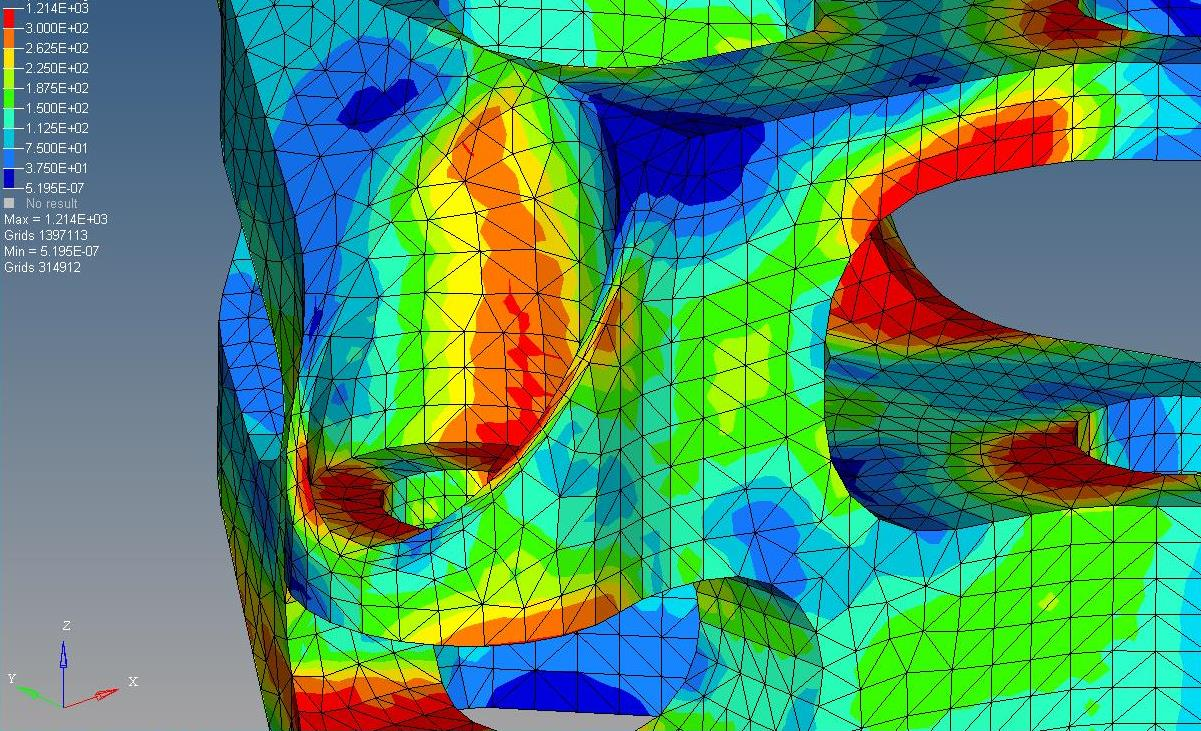
\includegraphics[width=5cm]{fem_sample} \\
      {\tiny Image: (c) PyCAE} 
    \end{center}
    
  \item One variable per cell
  \item A single equation \red{only} relates variables of \red{neighboring} cells
  \item $Ax = b$ with \red{sparse} A (mostly zero coefficients)
  \end{itemize}
\end{frame}

%%%%%%%%%%%%%%%%%%%%%%%%%%%%%%%%%%%%%%%%%%%%

\begin{frame}
  \frametitle{Sparse Matrices}

  \begin{block}{Goals when dealing with sparse matrices}
    \begin{itemize}
    \item Don't store 0
    \item Don't compute $0 + x$ and $0 \times x$
    \end{itemize}
  \end{block}
  
  \begin{center}
    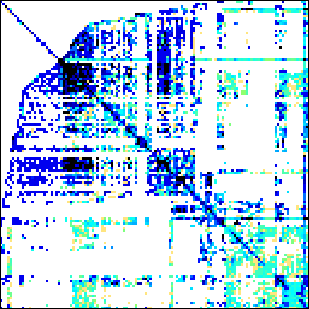
\includegraphics[width=3cm]{sparse.png} \\
    {\tiny Image: (c) T. davis} 
  \end{center}
  
  \begin{block}{Most important parameter: \textbf{density}}
    \begin{itemize}
    \item Proportion of \red{non-zero} coefficients
    \item density $< 0.01$ (say) $\leadsto$ sparse
    \end{itemize}
  \end{block}
  
\end{frame}

%%%%%%%%%%%%%%%%%%%%%%%%%%%%%%%%%%%%%%%%%%%%

\begin{frame}[fragile=singleslide]
\frametitle{Sparse Matrix Storage, Triplet Form}

\begin{exampleblock}{Simplest Possible Idea}
  List of triplets $(i, j, x)$ for each non-zero entry $A[i,j] = x$.
  
\begin{minted}[fontsize=\small]{C}
struct triplet {
    int n, m, nz;
    int nzmax;    /* allocated size for Ai, Aj, Ax */
    int *Ai;
    int *Aj;
    double *Ax;
};                /* note: order is irrelevant */
\end{minted}
\end{exampleblock}

\medskip

Assuming \mintinline{C}{int} indices ($i$, $j$) and \mintinline{C}{double} coefficients ($x$),
\[
\mintinline{c}{sizeof(A)} =  16 |A| + 16 \texttt{ bytes} \qquad\text{(regardless of $n, m$)}
\]

\end{frame}

%%%%%%%%%%%%%%%%%%%%%%%%

\begin{frame}[fragile=singleslide]
\frametitle{Sparse Matrix Storage, Triplet Form (continued)}

\begin{block}{Pros}
  \begin{itemize}
  \item Friendly format for I/O
  \item Repeated $i,j$ can be allowed (coefficients are summed)
  \end{itemize}
\end{block}

Possible file format :
\begin{verbatim}
n m
i_0 j_0 x_0
i_1 j_1 x_1
.....
\end{verbatim}


\begin{alertblock}{Cons}
  \begin{itemize}
  \item Limited operations. $x \gets A[i,j]$ is impossible!
  \end{itemize}
\end{alertblock}
\end{frame}

%%%%%%%%%%%

\begin{frame}[fragile]
\frametitle{Storage, Triplet Form, Operations}

\begin{itemize}
\item $A \gets A^t$
\item<2-> $A \gets \lambda A$
\item<3-> $y \gets y + x A$
\item<4-> $y \gets y + A x$
\item<5-> $A \gets P A Q$
\item<6-> $A \gets B + C$
\end{itemize}



\begin{overlayarea}{\textwidth}{3cm}
\begin{onlyenv}<1>
\begin{minted}{C}
int *tmp = Ai;      /* constant-time! */
Ai = Aj;
Aj = tmp;
\end{minted}
\end{onlyenv}

\begin{onlyenv}<2>
\begin{minted}{C}
for (int p = 0; p < nz; p++)
    Ax[p] *= lambda;
\end{minted}
\end{onlyenv}

\begin{onlyenv}<3>
\begin{minted}{C}
for (int p = 0; p < nz; p++)
    y[Aj[p]] += x[Ai[p]] * Ax[p];       
\end{minted}
\end{onlyenv}

\begin{onlyenv}<4>
\begin{minted}{C}
for (int p = 0; p < nz; p++)
    y[Ai[p]] += x[Aj[p]] * Ax[p];       
\end{minted}
\end{onlyenv}

\begin{onlyenv}<5>
\begin{minted}{C}
for (int p = 0; p < nz; p++) {
    Ai[p] = Pinv[Ai[p]];
    Aj[p] = Qinv[Aj[p]];
}
\end{minted}
\end{onlyenv}

\begin{onlyenv}<6>
  \medskip

  Essentially concatenate $B$ and $C$.
\end{onlyenv}


\begin{alertblock}<7>{Main Limitations}
  \begin{itemize}
  \item Everything else is impossible!
  \item Wasteful storage
  \end{itemize}
\end{alertblock}

\end{overlayarea}
\end{frame}

%%%%%%%%%%%%%%%%%%%%%%%%%

\begin{frame}[fragile]
\frametitle{Storage, Compressed Sparse Rows (CSR) Form}

\begin{exampleblock}{Pack Rows Together}
%  For each row $i$, list of pairs $(j, x)$ such that $A[i,j] = x$. 
\begin{minted}[fontsize=\small]{C}
struct csr {
    int n, m;
    int *Ap;     // row pointers   (size n+1)
    int *Aj;     // column indices (size nz)
    double *Ax;  // coefficients   (size nz)
};
\end{minted}
\end{exampleblock}

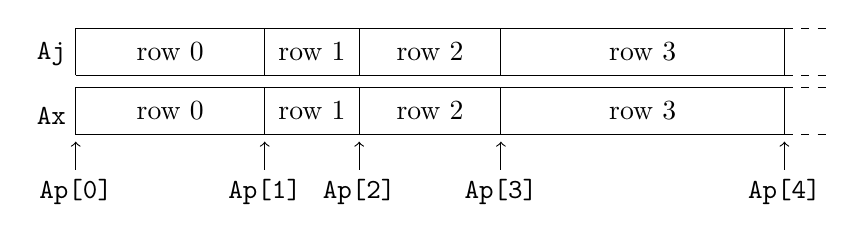
\begin{tikzpicture}[scale=0.6]
  \node[anchor=south east] at (0,0) {\texttt{Aj}};
  \draw (0, 0) -- (15, 0);
  \draw (0, 1) -- (15, 1);
  \draw (0, 0) -- (0, 1);
  \draw[dashed] (15, 0) -- +(1, 0);
  \draw[dashed] (15, 1) -- +(1, 0);

  \begin{scope}[yshift=-1.25cm]
    \node[anchor=south east] at (0,0) {\texttt{Ax}};
    \draw (0, 0) -- (15, 0);
    \draw (0, 1) -- (15, 1);
    \draw (0, 0) -- (0, 1);
    \draw[dashed] (15, 0) -- +(1, 0);
    \draw[dashed] (15, 1) -- +(1, 0);
  \end{scope}

  \draw (4, 0) -- +(0, 1);
  \path (0, 0) rectangle node {row 0} +(4, 1);
  \draw (6, 0) -- +(0, 1);
  
  \path (4, 0) rectangle node {row 1} +(2, 1);

  \draw (9, 0) -- +(0, 1);
  \path (6, 0) rectangle node {row 2} +(3, 1);

  \draw (15, 0) -- +(0, 1);
  \path (9, 0) rectangle node {row 3} +(6, 1);

  \begin{scope}[yshift=-1.25cm]
  \draw (4, 0) -- +(0, 1);
  \path (0, 0) rectangle node {row 0} +(4, 1);
  \draw (6, 0) -- +(0, 1);
  
  \path (4, 0) rectangle node {row 1} +(2, 1);

  \draw (9, 0) -- +(0, 1);
  \path (6, 0) rectangle node {row 2} +(3, 1);

  \draw (15, 0) -- +(0, 1);
  \path (9, 0) rectangle node {row 3} +(6, 1);
\end{scope}

\draw[->] (0, -2) node[anchor=north,font=\ttfamily] {Ap[0]} -- (0, -1.4);
\draw[->] (4, -2) node[anchor=north,font=\ttfamily] {Ap[1]} -- (4, -1.4);
\draw[->] (6, -2) node[anchor=north,font=\ttfamily] {Ap[2]} -- (6, -1.4);
\draw[->] (9, -2) node[anchor=north,font=\ttfamily] {Ap[3]} -- (9, -1.4);
\draw[->] (15, -2) node[anchor=north,font=\ttfamily] {Ap[4]} -- (15, -1.4);
\end{tikzpicture}

%\vspace{-0.5cm}
\[
\mintinline{c}{sizeof(A)} =  12 |A| + 4n + 12 \texttt{ bytes} \qquad\text{(regardless of $m$)}
\]


% \begin{block}{Iterating over row $i$}
% \begin{minted}{c}
%   for (int p = Ap[i]; p < Ap[i + 1]; p++) {
%             int j = Aj[p];
%             int x = Ax[p];
%             ...
% \end{minted}
% \end{block}
\end{frame}


\begin{frame}[fragile]
\frametitle{Storage, CSR Form, Operations}

\begin{itemize}
\item $x \gets |A|$  
\item<2-> $y \gets y + x A$
\item<3-> $y \gets y + A x$
\item<4-> $A \gets A Q$
\end{itemize}

\begin{overlayarea}{\textwidth}{3cm}

\begin{onlyenv}<1>
\begin{minted}{C}
  x = Ap[n + 1];
\end{minted}
\end{onlyenv}

\begin{onlyenv}<2>
\begin{minted}{C}
for (int i = 0; i < n; i++)
    for (int p = Ap[i]; p < Ap[i + 1]; p++)
        y[Aj[p]] += x[i] * Ax[p];
\end{minted}
\end{onlyenv}

\begin{onlyenv}<3>
\begin{minted}{C}
for (int i = 0; i < n; i++)
    for (int p = Ap[i]; p < Ap[i + 1]; p++)
        y[i] += x[Aj[p]] * Ax[p];
\end{minted}
\end{onlyenv}

\begin{onlyenv}<4>
\begin{minted}{C}
for (int p = 0; p < Ap[n + 1]; p++)
    Aj[p] = Qinv[Aj[p]];
\end{minted}
\end{onlyenv}

\begin{block}<only@5>{Remarks}
  \begin{itemize}
  \item Order of entries in row irrelevant
  \item Duplicates are allowed (but wasteful)
  \item Explicit 0 entries are allowed (but wasteful)
  \end{itemize}
\end{block}


\begin{alertblock}<6>{Main Limitation}
  \begin{itemize}
  \item Transpose, row permutation not in place.
    \begin{itemize}      
    \item Lazy solution: convert to triplets, work, convert back to CSR
    \end{itemize}
  \item $x \gets A[i,j]$ still impossible... 
    \begin{itemize}      
    \item Direct access to rows/iteration over rows is possible.
    \end{itemize}

  \end{itemize}
\end{alertblock}
\end{overlayarea}
\end{frame}

%%%%%%%%%%%%%%%%%%%%%%%%%%%%%%%%%%%%%%%%%%%


%%%%%%%%%%%%%%%%%%%%%%%%%%%%%%%%%%%%%%%%%%%%

\begin{frame}[fragile=singleslide]
  \frametitle{Matrix-Vector product (\texttt{GEMV})}
  \framesubtitle{$y \gets y + \alpha Ax$}
  \begin{alertblock}{Dense \texttt{GEMV}}
    \begin{itemize}
    \item All matrix coeffs are contiguous in memory
    \end{itemize}
    \vspace*{-2ex}
    \begin{minted}[fontsize=\small]{C}
for (int i = 0; i < n; i++)               // 3nm FLOP
    for (int j = 0; j < m; j++)
        y[i] += alpha * A[i*m + j] * x[j]; 
      \end{minted}
    \end{alertblock}
  
  \begin{exampleblock}{Sparse \texttt{GEMV}}
      \begin{minted}[fontsize=\small]{C}
for (int k = 0; k < nz; k++)              // 3nz FLOP
    y[Ai[k]] += alpha * Ax[k] * x[Aj[k]]; 
    \end{minted}
  \end{exampleblock}
\end{frame}

%%%%%%%%%%%%%%%%%%%%%%%%%%%%%%%%%%%%%%%%%%%% 
\subsubsection{Iteratove methods}
\begin{frame}
  \frametitle{Recurring problem in HPC}

  \begin{block}{Iterative methods with sparse matrices}
    \begin{itemize}
    \item compute $x_{i+1} = A x_i$
    \item For $i=1, 2, 3,  4, 5, \dots$
    \item With large, sparse matrix $A$
    \item \red{In parallel}
      \begin{itemize}
      \item Need $x_{i+1}$ to start $x_{i+2}$
      \item Iterations are necessarily \red{sequential} 
      \item[$\Rightarrow$] Parallelize the \textbf{matrix-vector product}
      \end{itemize}
    \end{itemize}
  \end{block}  
  
  \begin{exampleblock}{Data parallelism}
    \begin{itemize}
    \item $A$ is \textbf{distributed} between processes (how?)
    \item $x_i$ is \textbf{distributed} between processes (how?)
    \item $x_{i+1}$ must be distributed \red{identically} to iterate
    \end{itemize}
  \end{exampleblock}
  
\end{frame}

%%%%%%%%%%%%%%%%%%%%%%%%%%%%%%%%%%%%%%%%%%%

\begin{frame}[label=1d]
  \frametitle{Distributed Matrix-Vector Product}
  \framesubtitle{1D block distribution (per rows)}

  \begin{block}{Data distribution}
    \begin{itemize}
    \item[$M$] : 1D block distribution (blocks of rows)
    \item[$x$] : owned by all processes
    \item[$y$] : owned by all processes
    \end{itemize}
  \end{block}


  \begin{center}
    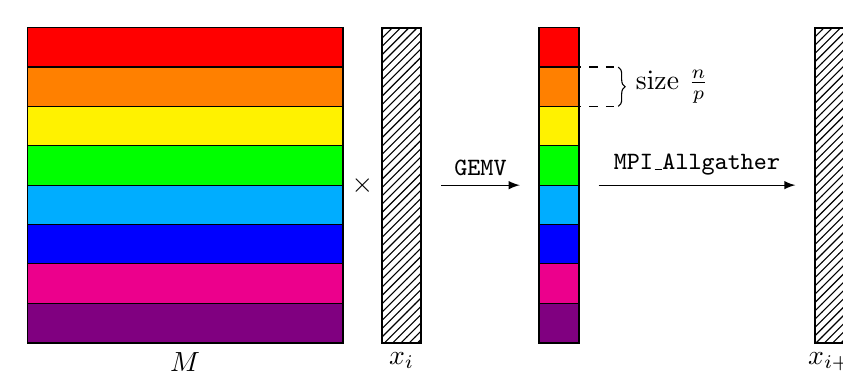
\begin{tikzpicture}[>=latex]
      \path[red,dotted,use as bounding box] (0,0) rectangle (10, 4);
      \draw[<->] (-0.5,0) -- node[left] {$n$} +(0, 4);
  
      % matrix
      \draw[thick] (0,0) rectangle (4,4);
      \filldraw[fill=red]     (0, 3.5) rectangle +(4, 0.5);
      \filldraw[fill=orange]  (0, 3  ) rectangle +(4, 0.5);
      \filldraw[fill=yellow]  (0, 2.5) rectangle +(4, 0.5);
      \filldraw[fill=green]   (0, 2  ) rectangle +(4, 0.5);
      \filldraw[fill=cyan]    (0, 1.5) rectangle +(4, 0.5);
      \filldraw[fill=blue]    (0, 1  ) rectangle +(4, 0.5);
      \filldraw[fill=magenta] (0, 0.5) rectangle +(4, 0.5);
      \filldraw[fill=violet]  (0, 0  ) rectangle +(4, 0.5);
      
      \node[below] at (2,0) {$M$};

      \node at (4.25,2) {$\times$};
      
      \draw[thick,pattern=north east lines] (4.5,0) rectangle +(0.5,4);
      \node[below] at (4.75,0) {$x_i$};
      
      \draw[->] (5.25, 2) -- node[above,font=\small] {\texttt{GEMV}} +(1 ,0);

      \begin{scope}[xshift=0.5cm]
        \draw[thick] (6,0) rectangle +(0.5,4);
        \filldraw[fill=red]     (6, 3.5) rectangle +(0.5, 0.5);
        \filldraw[fill=orange]  (6, 3  ) rectangle +(0.5, 0.5);
        \filldraw[fill=yellow]  (6, 2.5) rectangle +(0.5, 0.5);
        \filldraw[fill=green]   (6, 2  ) rectangle +(0.5, 0.5);
        \filldraw[fill=cyan]    (6, 1.5) rectangle +(0.5, 0.5);
        \filldraw[fill=blue]    (6, 1  ) rectangle +(0.5, 0.5);
        \filldraw[fill=magenta] (6, 0.5) rectangle +(0.5, 0.5);
        \filldraw[fill=violet]  (6, 0  ) rectangle +(0.5, 0.5);
      \end{scope}

    \draw[->] (7.25, 2) -- node[above,font=\small] {\texttt{\texttt{MPI\_Allgather}}} +(2.5, 0);
      
      \draw[dashed] (6.5, 3) -- +(1, 0);
      \draw[dashed] (6.5, 3.5) -- +(1, 0);
      \draw[decorate,decoration={brace,mirror}] (7.5, 3) --  node[right=1mm] {size $\frac{n}{p}$} +(0, 0.5);

      % x_i+1
      \draw[thick,pattern=north east lines] (10,0) rectangle +(0.5,4);
      \node[below] at (10.25,0) {$x_{i+1}$};
    \end{tikzpicture}
  \end{center}
\end{frame}

%%%%%%%%%%%%%%%%%%%%%%%%%%%%%%%%%%%%%%%%%%%

\begin{frame}[label=1d]
%  \frametitle{Distributed Matrix-Vector Product (1D per rows)}

  \begin{alertblock}{Machine parameters}
    \begin{itemize}
    \item $C$ = processor FLOP/s
    \item $D$ = network bandwidth (float / s)
    \end{itemize}
  \end{alertblock}

  \begin{exampleblock}{Matrix characteristics}
    \begin{itemize}
    \item $n$ = size
    \item $d$ = \emph{density} ($dn^2$ non-zero coeffs)
%    \item[$\Rightarrow$] $3 d n^2$ FLOP / iteration
    \end{itemize}
  \end{exampleblock}

  \begin{center}
    \begin{tabular}{|c||c|c|}
      \hline
      & \texttt{GEMV}  & \texttt{MPI\_Allgather} \\
      \hline\hline
      Sequential           & $3 d n^2 / C$ &    0 \\
      \hline
      Distributed          & $3 d n^2 / (pC)$ & $\geq n / D$ \\
      \hline
    \end{tabular}
  \end{center}

  \[
    \mathrm{Speedup} \leq \frac{d n^2}{C} / (\frac{d n^2}{pC} + \frac{n}{D}) \leq d n \frac{D}{C}
  \]

  \begin{itemize}
  \item $D/C$ = ``machine balance'' = very important
 \end{itemize}
\end{frame}

%%%%%%%%%%%%%%%%%%%%%%%%%%%%%%%%%%%%%%%% 

\begin{frame}[label=1d]
  \frametitle{Communication Limits Acceleration}
  
  \begin{center}
    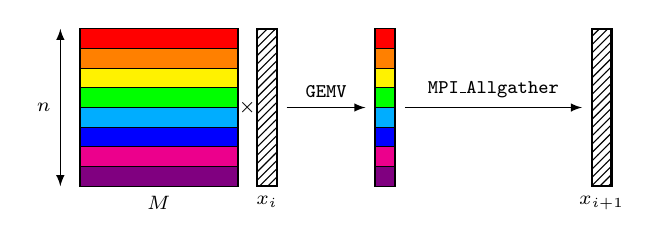
\begin{tikzpicture}[scale=0.5, >=latex, every node/.style={font=\scriptsize}]
      \draw[<->] (-0.5,0) -- node[left] {$n$} +(0, 4);
  
      % matrix
      \draw[thick] (0,0) rectangle (4,4);
      \filldraw[fill=red]     (0, 3.5) rectangle +(4, 0.5);
      \filldraw[fill=orange]  (0, 3  ) rectangle +(4, 0.5);
      \filldraw[fill=yellow]  (0, 2.5) rectangle +(4, 0.5);
      \filldraw[fill=green]   (0, 2  ) rectangle +(4, 0.5);
      \filldraw[fill=cyan]    (0, 1.5) rectangle +(4, 0.5);
      \filldraw[fill=blue]    (0, 1  ) rectangle +(4, 0.5);
      \filldraw[fill=magenta] (0, 0.5) rectangle +(4, 0.5);
      \filldraw[fill=violet]  (0, 0  ) rectangle +(4, 0.5);
      
      \node[below] at (2,0) {$M$};

      \node at (4.25,2) {$\times$};
      
      \draw[thick,pattern=north east lines] (4.5,0) rectangle +(0.5,4);
      \node[below] at (4.75,0) {$x_i$};
      
      \draw[->] (5.25, 2) -- node[above,font=\scriptsize] {\texttt{GEMV}} +(2 ,0);

      \begin{scope}[xshift=7.5cm]
        \draw[thick] (0,0) rectangle +(0.5,4);
        \filldraw[fill=red]     (0, 3.5) rectangle +(0.5, 0.5);
        \filldraw[fill=orange]  (0, 3  ) rectangle +(0.5, 0.5);
        \filldraw[fill=yellow]  (0, 2.5) rectangle +(0.5, 0.5);
        \filldraw[fill=green]   (0, 2  ) rectangle +(0.5, 0.5);
        \filldraw[fill=cyan]    (0, 1.5) rectangle +(0.5, 0.5);
        \filldraw[fill=blue]    (0, 1  ) rectangle +(0.5, 0.5);
        \filldraw[fill=magenta] (0, 0.5) rectangle +(0.5, 0.5);
        \filldraw[fill=violet]  (0, 0  ) rectangle +(0.5, 0.5);
      \end{scope}

    \draw[->] (8.25, 2) -- node[above,font=\scriptsize] {\texttt{MPI\_Allgather}} +(4.5, 0);
      
      % x_i+1
      \draw[thick,pattern=north east lines] (13,0) rectangle +(0.5,4);
      \node[below] at (13.25,0) {$x_{i+1}$};
    \end{tikzpicture}
  \end{center}

\vspace{0.5cm}
  
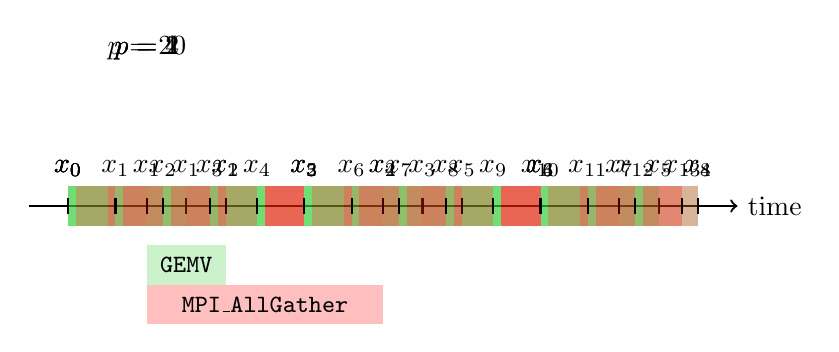
\begin{tikzpicture}
    \node<1> at (1, 2) {$p=1$};
    \node<2> at (1, 2) {$p=2$};
    \node<3> at (1, 2) {$p=4$};
    \node<4> at (1, 2) {$p=20$};
    
    \draw[thick, ->] (-0.5, 0) -- (8.5, 0) node[right] {time};

    
    \foreach \i in {0, 1, 2, 3}  {
      \fill<1>[fill=LimeGreen, nearly transparent] (\i*2cm, -0.25) rectangle +(2, 0.5);
    }
    \foreach \i in {0, 1, 2, 3, 4} {
      \draw<1>[thick] (\i*2cm, -0.1) -- +(0, 0.2);
      \node<1>[anchor=south] at (\i*2cm, 0.25) {$x_\i$};
    }

    % p = 2
    \foreach \i in {0, 1, 2, 3, 4}  {
      \fill<2>[fill=LimeGreen, nearly transparent] (\i*1.5cm, -0.25) rectangle +(1, 0.5);
      \fill<2>[fill=red, nearly transparent] (\i*1.5cm, 0) +(1, -0.25) rectangle +(1.5, 0.25);
    }
    \foreach \i in {0, 1, 2, 3, 4, 5} {
      \draw<2>[thick] (\i*1.5cm, -0.1) -- +(0, 0.2);
      \node<2>[anchor=south] at (\i*1.5cm, 0.25) {$x_\i$};
    }

    % p = 4
    \foreach \i in {0, 1, 2, ..., 7}  {
      \fill<3>[fill=LimeGreen, nearly transparent] (\i*1cm, -0.25) rectangle +(0.5, 0.5);
      \fill<3>[fill=red, nearly transparent] (\i*1cm+0.5cm, -0.25)  rectangle +(0.5, 0.5);
    }
    \foreach \i in {0, 1, ..., 8} {
      \draw<3>[thick] (\i*1cm, -0.1) -- +(0, 0.2);
      \node<3>[anchor=south] at (\i*1cm, 0.25) {$x_\i$};
    }

    % p = 20
    \foreach \i in {0, 1, 2, ..., 12}  {
      \fill<4>[fill=LimeGreen, nearly transparent] (\i*0.6cm, -0.25) rectangle +(0.1, 0.5);
      \fill<4>[fill=red, nearly transparent] (\i*0.6cm+0.1cm, -0.25)  rectangle +(0.5, 0.5);
    }
    \foreach \i in {0, 1, ..., 13} {
      \draw<4>[thick] (\i*0.6cm, -0.1) -- +(0, 0.2);
      \node<4>[anchor=south] at (\i*0.6cm, 0.25) {$x_{\i}$};
    }

    
    \fill[fill=LimeGreen, nearly transparent] (1, -1) rectangle +(1, 0.5);
    \path (1, -1) rectangle node[font=\small] {\texttt{GEMV}} +(1, 0.5);

    \fill[fill=red, nearly transparent] (1, -1.5) rectangle +(3, 0.5);
    \path (1, -1.5) rectangle node[font=\small] {\texttt{MPI\_AllGather}} +(3, 0.5);
  \end{tikzpicture}
\end{frame}


%%%%%%%%%%%%%%%%%%%%%%%%%%%%%%%%%%%%%%%%%%% 

\begin{frame}
  \frametitle{Distributed Matrix-Vector Product}
  \framesubtitle{1D block distribution (per columns)}

  \begin{block}{Data distribution}
    \begin{itemize}
    \item[$M$] : 1D block distribution (blocks of columns)
    \item[$x$] : 1D block distribution
    \item[$y$] : 1D block distribution
    \end{itemize}
  \end{block}


  \begin{center}
    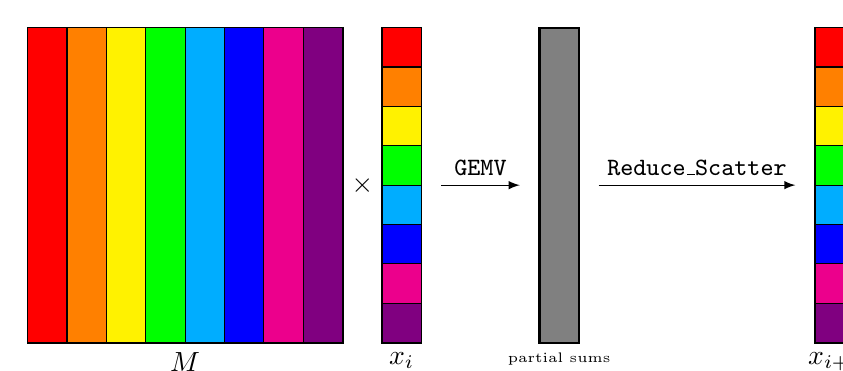
\begin{tikzpicture}[>=latex]
      \path[red,dotted,use as bounding box] (0,0) rectangle (10, 4);
      \draw[<->] (-0.5,0) -- node[left] {$n$} +(0, 4);
  
      % matrix
      \draw[thick] (0,0) rectangle (4,4);
      \filldraw[fill=red]     (0  , 0) rectangle +(0.5, 4);
      \filldraw[fill=orange]  (0.5, 0) rectangle +(0.5, 4);
      \filldraw[fill=yellow]  (1.0, 0) rectangle +(0.5, 4);
      \filldraw[fill=green]   (1.5, 0) rectangle +(0.5, 4);
      \filldraw[fill=cyan]    (2.0, 0) rectangle +(0.5, 4);
      \filldraw[fill=blue]    (2.5, 0) rectangle +(0.5, 4);
      \filldraw[fill=magenta] (3.0, 0) rectangle +(0.5, 4);
      \filldraw[fill=violet]  (3.5, 0) rectangle +(0.5, 4);
      
      \node[below] at (2,0) {$M$};

      \node at (4.25,2) {$\times$};
      
      \begin{scope}[xshift=4.5cm]
        \draw[thick] (0,0) rectangle +(0.5,4);
        \filldraw[fill=red]     (0, 3.5) rectangle +(0.5, 0.5);
        \filldraw[fill=orange]  (0, 3  ) rectangle +(0.5, 0.5);
        \filldraw[fill=yellow]  (0, 2.5) rectangle +(0.5, 0.5);
        \filldraw[fill=green]   (0, 2  ) rectangle +(0.5, 0.5);
        \filldraw[fill=cyan]    (0, 1.5) rectangle +(0.5, 0.5);
        \filldraw[fill=blue]    (0, 1  ) rectangle +(0.5, 0.5);
        \filldraw[fill=magenta] (0, 0.5) rectangle +(0.5, 0.5);
        \filldraw[fill=violet]  (0, 0  ) rectangle +(0.5, 0.5);
      \end{scope}

      \node[below] at (4.75,0) {$x_i$};
      
      \draw[->] (5.25, 2) -- node[above,font=\small] {\texttt{GEMV}} +(1 ,0);

      \draw[thick,fill=gray] (6.5,0) rectangle +(0.5,4);
      \node[below] at (6.75,0) {\tiny partial sums};

      
      \draw[->] (7.25, 2) -- node[above,font=\small] {\texttt{\texttt{Reduce\_Scatter}}} +(2.5, 0);
      
      % x_i+1
      \begin{scope}[xshift=10cm]
        \draw[thick] (0,0) rectangle +(0.5,4);
        \filldraw[fill=red]     (0, 3.5) rectangle +(0.5, 0.5);
        \filldraw[fill=orange]  (0, 3  ) rectangle +(0.5, 0.5);
        \filldraw[fill=yellow]  (0, 2.5) rectangle +(0.5, 0.5);
        \filldraw[fill=green]   (0, 2  ) rectangle +(0.5, 0.5);
        \filldraw[fill=cyan]    (0, 1.5) rectangle +(0.5, 0.5);
        \filldraw[fill=blue]    (0, 1  ) rectangle +(0.5, 0.5);
        \filldraw[fill=magenta] (0, 0.5) rectangle +(0.5, 0.5);
        \filldraw[fill=violet]  (0, 0  ) rectangle +(0.5, 0.5);
      \end{scope}


      \node[below] at (10.25,0) {$x_{i+1}$};
    \end{tikzpicture}
  \end{center}
\end{frame}

%%%%%%%%%%%%%%%%%%%%%%%%%%%%%%%%%%%%%%%%%%%%%%%%%%%%%%%%%%%%%%%%

\begin{frame}[fragile=singleslide]
\frametitle{MPI : Reduce-Scatter}

  \begin{wider}
\begin{minted}[fontsize=\footnotesize]{C}
int MPI_Reduce_scatter_block(void* sendbuf, void* recvbuf,
                             int recvcount, MPI_Datatype datatype,
                             MPI_Op op, MPI_Comm comm)
\end{minted}
  \end{wider}

  \bigskip

  \begin{center}
    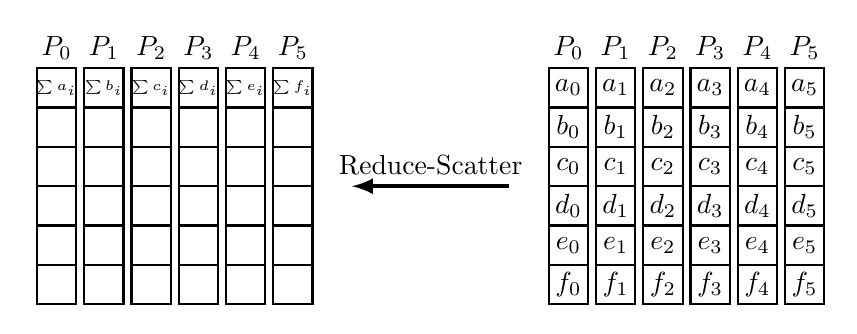
\begin{tikzpicture}[scale=0.5, >=latex]
            \begin{scope}
        \foreach \letter / \i in {a / 0, b / 1, c / 2, d / 3, e / 4, f / 5} {
          \draw[thick] (1.2*\i, 0) rectangle +(1, 6);
          \foreach \j in {1,...,5} {
            \draw[thick] (1.2*\i, \j) -- +(1, 0);
          }
          \node at (1.2*\i + 0.5, 6.5) {$P_\i$};          
          \node at (0.5 + 1.2*\i, 5.5) {$\scriptscriptstyle \sum \letter_i$};
        }
      \end{scope}

      \draw[ultra thick,<-] (8, 3) -- node[above] {Reduce-Scatter} (12, 3);

      \begin{scope}[xshift=13cm]
        \foreach \letter / \i in {a / 0, b / 1, c / 2, d / 3, e / 4, f / 5} {
          \draw[thick] (1.2*\i, 0) rectangle +(1, 6);
          \foreach \j in {1,...,5} {
            \draw[thick] (1.2*\i, \j) -- +(1, 0);
          }
          \node at (1.2*\i + 0.5, 6.5) {$P_\i$};
          \foreach \j in {0,1,...,5} {
            \node<1> at (0.5 + 1.2*\j,  5.5 - \i) {$\letter_\j$};
          }
        }
      \end{scope}
\end{tikzpicture}
\end{center}

\begin{itemize}
\item Lower bound: $T \geq \lceil \log_2 p \rceil \alpha + (p-1) \frac{n}{p} \beta$
\item Ring algorithm: $T = (p-1) (\alpha + \frac{n}{p} \beta)$
\end{itemize}

\end{frame}



%%%%%%%%%%%%%%%%%%%%%%%%%%%%%%%%%%%%%%%%%%%%

\begin{frame}[label=2d]
  \frametitle{Distributed Matrix-Vector Product}
  \framesubtitle{2D block distribution}

  \begin{block}{Data distribution}
    \begin{itemize}
    \item[$M$] : 2D block distribution ($v \times h$ blocks)
    \item[$x$] : 1D block distribution 
    \item[$y$] : 1D block distribution
    \end{itemize}
  \end{block}

  \begin{center}
    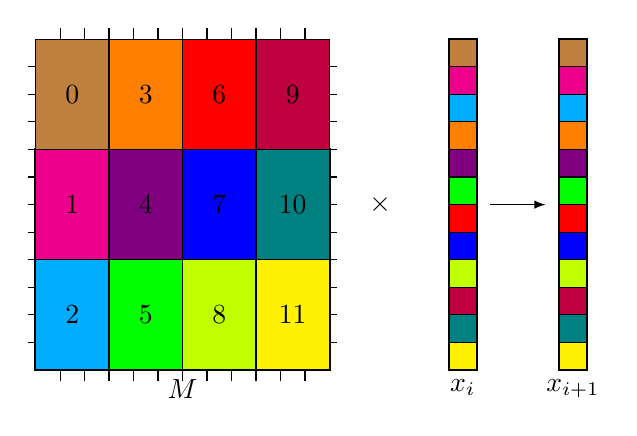
\begin{tikzpicture}[>=latex, scale=0.7]
      \begin{scope}[xshift=-4cm, yscale=2, xscale=1.333]
        \draw[thick] (0,0) rectangle (4,2);
        \foreach \i in {1, 2, ..., 11} {
          \draw (-0.1, \i/4) -- (0, \i/4);
          \draw (\i/3, -0.1) -- (\i/3, 0);
          \draw (4.1, \i/4) -- (4, \i/4);
          \draw (\i/3, 3.1) -- (\i/3, 3);
        }
      \filldraw[fill=brown]    (0, 2) rectangle node {0} +(1, 1);
      \filldraw[fill=orange]   (1, 2) rectangle  node {3} +(1, 1);
      \filldraw[fill=red]      (2, 2) rectangle  node {6} +(1, 1);
      \filldraw[fill=purple]   (3, 2) rectangle  node {9} +(1, 1);
      \filldraw[fill=magenta]  (0, 1) rectangle  node {1} +(1, 1);
      \filldraw[fill=violet]   (1, 1) rectangle  node {4} +(1, 1);
      \filldraw[fill=blue]     (2, 1) rectangle  node {7} +(1, 1);
      \filldraw[fill=teal]     (3, 1) rectangle  node {10} +(1, 1);
      \filldraw[fill=cyan]     (0, 0) rectangle  node {2} +(1, 1);
      \filldraw[fill=green]    (1, 0) rectangle  node {5} +(1, 1);
      \filldraw[fill=lime]     (2, 0) rectangle  node {8} +(1, 1);
      \filldraw[fill=yellow]   (3, 0) rectangle  node {11} +(1, 1);

      \node[below] at (2,0) {$M$};
    \end{scope}

    \node at (2.25, 3) {$\times$};

          \begin{scope}[xshift=-1cm]
      \draw[thick] (4.5,0) rectangle +(0.5, 6);
      \filldraw[fill=brown]    (4.5, 5.5) rectangle   +(0.5, 0.5);
      \filldraw[fill=magenta]   (4.5, 5) rectangle     +(0.5, 0.5);
      \filldraw[fill=cyan]     (4.5, 4.5) rectangle   +(0.5, 0.5);
      \filldraw[fill=orange]    (4.5, 4) rectangle     +(0.5, 0.5);
      \filldraw[fill=violet]  (4.5, 3.5) rectangle   +(0.5, 0.5);
      \filldraw[fill=green]   (4.5, 3) rectangle     +(0.5, 0.5);
      \filldraw[fill=red]     (4.5, 2.5) rectangle   +(0.5, 0.5);
      \filldraw[fill=blue]     (4.5, 2) rectangle     +(0.5, 0.5);
      \filldraw[fill=lime]      (4.5, 1.5) rectangle   +(0.5, 0.5);
      \filldraw[fill=purple]    (4.5, 1) rectangle     +(0.5, 0.5);
      \filldraw[fill=teal]     (4.5, 0.5) rectangle   +(0.5, 0.5);
      \filldraw[fill=yellow]   (4.5, 0) rectangle     +(0.5, 0.5);
      \node[below] at (4.75,0) {$x_i$};
    \end{scope}
    \draw[->] (4.25, 3) -- +(1,0);
      
      \begin{scope}[xshift=1cm]
              \draw[thick] (4.5,0) rectangle +(0.5, 6);
      \filldraw[fill=brown]    (4.5, 5.5) rectangle   +(0.5, 0.5);
      \filldraw[fill=magenta]   (4.5, 5) rectangle     +(0.5, 0.5);
      \filldraw[fill=cyan]     (4.5, 4.5) rectangle   +(0.5, 0.5);
      \filldraw[fill=orange]    (4.5, 4) rectangle     +(0.5, 0.5);
      \filldraw[fill=violet]  (4.5, 3.5) rectangle   +(0.5, 0.5);
      \filldraw[fill=green]   (4.5, 3) rectangle     +(0.5, 0.5);
      \filldraw[fill=red]     (4.5, 2.5) rectangle   +(0.5, 0.5);
      \filldraw[fill=blue]     (4.5, 2) rectangle     +(0.5, 0.5);
      \filldraw[fill=lime]      (4.5, 1.5) rectangle   +(0.5, 0.5);
      \filldraw[fill=purple]    (4.5, 1) rectangle     +(0.5, 0.5);
      \filldraw[fill=teal]     (4.5, 0.5) rectangle   +(0.5, 0.5);
      \filldraw[fill=yellow]   (4.5, 0) rectangle     +(0.5, 0.5);
      \node[below] at (4.75,0) {$x_{i+1}$};
    \end{scope}

  \end{tikzpicture}
\end{center}
\end{frame}

%%%%%%%%%%%%%%%%%%%%%%%%%%%%%%%%%%%

\begin{frame}[label=2d]
  \begin{columns}
    \begin{column}{6cm}
    \begin{tikzpicture}[>=latex,scale=0.4]
      \begin{scope}[xshift=-4cm, yscale=2, xscale=1.5]
        \foreach \i in {1, 2, ..., 11} {
          \draw (-0.1, \i/4) -- (0, \i/4);
          \draw (\i/3, -0.1) -- (\i/3, 0);
          \draw (4.1, \i/4) -- (4, \i/4);
          \draw (\i/3, 3.1) -- (\i/3, 3);
        }
      \filldraw[fill=brown]    (0, 2) rectangle node {0} +(1, 1);
      \filldraw[fill=orange]   (1, 2) rectangle  node {3} +(1, 1);
      \filldraw[fill=red]      (2, 2) rectangle  node {6} +(1, 1);
      \filldraw[fill=purple]   (3, 2) rectangle  node {9} +(1, 1);
      \filldraw[fill=magenta]  (0, 1) rectangle  node {1} +(1, 1);
      \filldraw[fill=violet]   (1, 1) rectangle  node {4} +(1, 1);
      \filldraw[fill=blue]     (2, 1) rectangle  node {7} +(1, 1);
      \filldraw[fill=teal]     (3, 1) rectangle  node {10} +(1, 1);
      \filldraw[fill=cyan]     (0, 0) rectangle  node {2} +(1, 1);
      \filldraw[fill=green]    (1, 0) rectangle  node {5} +(1, 1);
      \filldraw[fill=lime]     (2, 0) rectangle  node {8} +(1, 1);
      \filldraw[fill=yellow]   (3, 0) rectangle  node {11} +(1, 1);
      \draw[thick] (0,0) rectangle (4, 3);
      
      \draw<2>[pattern=north east lines] (0, 2) rectangle  +(1/3, 1);
      \draw<2>[pattern=north east lines] (1, 2) rectangle  +(1/3, 1);
      \draw<2>[pattern=north east lines] (2, 2) rectangle  +(1/3, 1);
      \draw<2>[pattern=north east lines] (3,   2) rectangle  +(1/3, 1);
      \draw<2>[pattern=north east lines] (1/3, 1) rectangle  +(1/3, 1);
      \draw<2>[pattern=north east lines] (1+1/3, 1) rectangle  +(1/3, 1);
      \draw<2>[pattern=north east lines] (2+1/3, 1) rectangle  +(1/3, 1);
      \draw<2>[pattern=north east lines] (3+1/3, 1) rectangle  +(1/3, 1);
      \draw<2>[pattern=north east lines] (0+2/3, 0) rectangle  +(1/3, 1);
      \draw<2>[pattern=north east lines] (1+2/3, 0) rectangle  +(1/3, 1);
      \draw<2>[pattern=north east lines] (2+2/3, 0) rectangle  +(1/3, 1);
      \draw<2>[pattern=north east lines] (3+2/3, 0) rectangle  +(1/3, 1);

      \node[below] at (2,0) {$M$};
    \end{scope}

    \begin{onlyenv}<9-10>
      \begin{scope}[xshift=4cm, yscale=2, xscale=1.5]
        \foreach \i in {1, 2, ..., 11} {
          \draw (-0.1, \i/4) -- (0, \i/4);
          \draw (\i/3, -0.1) -- (\i/3, 0);
          \draw (4.1, \i/4) -- (4, \i/4);
          \draw (\i/3, 3.1) -- (\i/3, 3);
        }
      \filldraw[fill=brown]    (0, 2) rectangle node {0} +(1, 1);
      \filldraw[fill=magenta]  (1, 2) rectangle  node {1} +(1, 1);
      \filldraw[fill=cyan]     (2, 2) rectangle  node {2} +(1, 1);      
      \filldraw[fill=orange]   (3, 2) rectangle  node {3} +(1, 1);
      
      \filldraw[fill=violet]   (0, 1) rectangle  node {4} +(1, 1);
      \filldraw[fill=green]    (1, 1) rectangle  node {5} +(1, 1);
      \filldraw[fill=red]      (2, 1) rectangle  node {6} +(1, 1);
      \filldraw[fill=blue]     (3, 1) rectangle  node {7} +(1, 1);
      
      \filldraw[fill=lime]     (0, 0) rectangle  node {8} +(1, 1);
      \filldraw[fill=purple]   (1, 0) rectangle  node {9} +(1, 1);
      \filldraw[fill=teal]     (2, 0) rectangle  node {10} +(1, 1);
      \filldraw[fill=yellow]   (3, 0) rectangle  node {11} +(1, 1);
      \draw[thick] (0,0) rectangle (4, 3);
    \end{scope}
  \end{onlyenv}
\end{tikzpicture}

    \begin{block}{Algorithm}
      \begin{itemize}
      \item<3-> \texttt{MPI\_Allgather}
      \item<5-> \texttt{GEMV} (partial sums)
      \item<7-> \texttt{MPI\_reduce\_scatter}
      \item<10-> \texttt{MPI\_sendrecv} (transpose)

      \end{itemize}
    \end{block}
  \end{column}

  \begin{column}{4cm}
    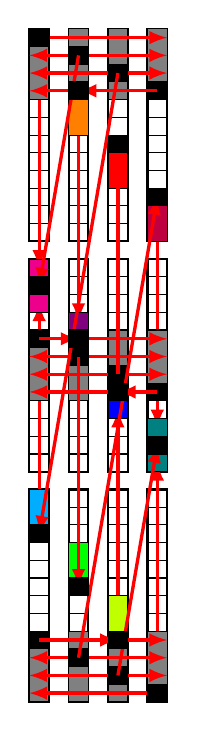
\begin{tikzpicture}[>=latex, yscale=0.45, xscale=0.5]
      % cadre
      \foreach \i in {0, 1, 2, 3} {
        \foreach \j in {0, 1, 2} {
          \draw[thick] (\i, 6.5*\j) rectangle +(0.5, 6);
          \foreach \k in {1, 2, ..., 11} {
            \draw (\i, 6.5*\j) ++(0, 0.5*\k) -- ++(0.5, 0);
          }
        }
      }

      % placement initial
      \foreach \i in {0, 1, 2, 3} {
        \foreach \j in {0, 1, 2} {
          \filldraw<1-3>[fill=black]  (\i, 3*6 + 0.5 - 1.5*\i - 7*\j)  rectangle +(0.5, 0.5);
        }
      }

      % Allgather colonnes arrows
      \draw<3>[red, very thick, <->] (0.25, 5.25 + 2*6.5) -- +(0, -6);
      \draw<3>[red, very thick, <->] (0.25, 4.75 + 1*6.5) -- +(0, -6);
      \draw<3>[red, very thick, <->] (1.25, 3.75 + 2*6.5) -- +(0, -6);
      \draw<3>[red, very thick, <->] (1.25, 3.25 + 1*6.5) -- +(0, -6);
      \draw<3>[red, very thick, <->] (2.25, 2.25 + 2*6.5) -- +(0, -6);
      \draw<3>[red, very thick, <->] (2.25, 1.75 + 1*6.5) -- +(0, -6);
      \draw<3>[red, very thick, <->] (3.25, 0.75 + 2*6.5) -- +(0, -6);
      \draw<3>[red, very thick, <->] (3.25, 0.25 + 1*6.5) -- +(0, -6);

      % allgather result
      \foreach \i in {0, 1, 2, 3} {
        \foreach \j in {0, 1, 2} {
          \filldraw<4>[fill=black]  (\i, 3*6 - 0.5 - 1.5*\i - 6.5*\j)  rectangle +(0.5, 1.5);
        }
      }

      % prepare GEMM
      \filldraw<5>[fill=brown]       (0, 17.5)   rectangle +(0.5, 1.5);
      \filldraw<5>[fill=orange]      (1, 16) rectangle +(0.5, 1.5);
      \filldraw<5>[fill=red]         (2, 14.5)   rectangle +(0.5, 1.5);
      \filldraw<5>[fill=purple]      (3, 13)   rectangle +(0.5, 1.5);
      \filldraw<5>[fill=magenta]     (0, 11)    rectangle +(0.5, 1.5);
      \filldraw<5>[fill=violet]      (1, 9.5)  rectangle +(0.5, 1.5);
      \filldraw<5>[fill=blue]        (2, 8)    rectangle +(0.5, 1.5);
      \filldraw<5>[fill=teal]        (3, 6.5)    rectangle +(0.5, 1.5);
      \filldraw<5>[fill=cyan]        (0, 4.5)    rectangle +(0.5, 1.5);
      \filldraw<5>[fill=green]       (1, 3)  rectangle +(0.5, 1.5);
      \filldraw<5>[fill=lime]        (2, 1.5)    rectangle +(0.5, 1.5);
      \filldraw<5>[fill=yellow]      (3, 0)    rectangle +(0.5, 1.5);


      % GEMM result
      \foreach \i in {0, 1, 2, 3} {
        \foreach \j in {0, 1, 2} {
          \filldraw<6-7>[fill=gray]  (\i, 2*\j + 6.5*\j)  rectangle +(0.5, 2);
        }
      }

      % Reduce-scatter arrow
      \foreach \i in {0, 1, 2, 3} {
        \foreach \j in {0, 1, 2} {
          \draw<7>[red,very thick, <->]  (0, 0.25 + 8.5*\j + 0.5*\i) -- +(3.5, 0);
        }
      }

      % placement après RS
      \foreach \i in {0, 1, 2, 3} {
        \foreach \j in {0, 1, 2} {
          \filldraw<8-10>[fill=black]  (\i, 1.5 - 0.5*\i +2*\j + 6.5*\j)  rectangle +(0.5, 0.5);
        }
      }

      % transposition
      \draw<10>[red, very thick,->]  (1.25, 5.25 + 2*6.5)  --  (0.25, 5.25 + 1*6.5);
      \draw<10>[red, very thick,->]  (2.25, 4.75 + 2*6.5)  --  (0.25, 4.75 + 0*6.5);
      \draw<10>[red, very thick,->]  (3.25, 4.25 + 2*6.5)  --  (1.25, 4.25 + 2*6.5);
      \draw<10>[red, very thick,->]  (0.25, 3.75 + 1*6.5)  --  (1.25, 3.75 + 1*6.5);
      \draw<10>[red, very thick,->]  (1.25, 3.25 + 1*6.5)  --  (1.25, 3.25 + 0*6.5);
      \draw<10>[red, very thick,->]  (2.25, 2.75 + 1*6.5)  --  (2.25, 2.75 + 2*6.5);
      \draw<10>[red, very thick,->]  (3.25, 2.25 + 1*6.5)  --  (2.25, 2.25 + 1*6.5);
      \draw<10>[red, very thick,->]  (0.25, 1.75 + 0*6.5)  --  (2.25, 1.75 + 0*6.5);
      \draw<10>[red, very thick,->]  (1.25, 1.25 + 0*6.5)  --  (3.25, 1.25 + 2*6.5);
      \draw<10>[red, very thick,->]  (2.25, 0.75 + 0*6.5)  --  (3.25, 0.75 + 1*6.5);

      % retour au placement initial
      \foreach \i in {0, 1, 2, 3} {
        \foreach \j in {0, 1, 2} {
          \filldraw<11>[fill=black]  (\i, 3*6 + 0.5 - 1.5*\i - 7*\j)  rectangle +(0.5, 0.5);
        }
      }
    \end{tikzpicture}
  \end{column}
\end{columns}
\end{frame}


%%%%%%%%%%%%%%%%%%%%%%%%%%%%%%%%

\begin{frame}[label=2d]
  \frametitle{Analysis}

  Process grid of size $p = P \times Q$
  
  \begin{center}
    \begin{tabular}{|c||c|c|}
      \hline
      & Sequential & Distributed \\
      \hline\hline
      \texttt{GEMV}                 & $3 d n^2 / C$ & $3 d n^2 / (pC)$ \\
      \hline
      \texttt{MPI\_Allgather}       & 0             & $n / (PD)$ \\
      \hline
      \texttt{MPI\_reduce\_scatter} & 0             & $n / (QD)$ \\
      \hline
      \texttt{MPI\_sendrecv}        & 0             & $n / (pD)$ \\
      \hline
    \end{tabular}
  \end{center}

  Assume $P = Q = \sqrt{p}$ and \alert{ignore latencies}:
  
  \[
    \mathrm{Speedup} = \frac{d n^2}{C} / \left(\frac{d n^2}{pC} + \frac{n}{D\sqrt{p}}\right)
  \]

  \begin{alertblock}{Progress}
    \begin{itemize}
    \item Communication time \textbf{also decreases} when $p$ grows
    \item Speed-up \textbf{no longer bounded} when $p$ grows
    \end{itemize}
  \end{alertblock}
  
\end{frame}


\end{document}






% Charles' emacs magic commands
%%% Local Variables:
%%% TeX-engine: xetex
%%% TeX-command-extra: "-shell-escape"
%%% TeX-command-extra-options: "-shell-escape"
%%% ispell-local-dictionary: "english"
%%% eval: (flyspell-mode 1)
%%% eval: (reftex-mode 1)
%%% End:
